%%%%%%%%%%%%%%%%%%%%%%%%%%%%%%%%%%%%%%%%%%%%%%%%%%%%%%%%%%%%%%%%%%%%%%%%%%%%%%%%
% PHD DISSERTATION
%
%
% Michael Malick
% 2016-11-03
% v0.01
%
%%%%%%%%%%%%%%%%%%%%%%%%%%%%%%%%%%%%%%%%%%%%%%%%%%%%%%%%%%%%%%%%%%%%%%%%%%%%%%%%

% DONE convert long tables --> tabular if the table is a single page
% DONE double check eq, fig, and table reference labels
% TODO integrate figures and tables into chapter text


% ----------------------------
% Pre-amble
% ----------------------------
% {{{

\documentclass[11pt]{report}
\usepackage{natbib}
\usepackage{pdflscape}
\usepackage{fancyhdr}
\usepackage{graphicx}
\usepackage{setspace}
\usepackage{pdfpages}
\usepackage{longtable}
\usepackage{booktabs}        % provides cmidrule
\usepackage{threeparttable}  % provides tablenotes
\usepackage{threeparttablex} % enables table notes with long tables
\usepackage[margin=1cm]{caption}
\usepackage[showframe=false, 
            includefoot,       % ensure page numbers do not extend into margins
            includehead,       % ensure page numbers do not extend into margins
            headheight=13.6pt, % need for fancyhdr
            top=1.0in, 
            bottom=1.0in, 
            left=1.25in, 
            right=1.25in ]{geometry}
\usepackage{hyperref}
\hypersetup{pdfstartview=FitH,
            bookmarksopen=false,
            colorlinks,
            linkcolor=black,
            urlcolor=black,
            citecolor=black}
\usepackage{amstext}
\usepackage{amsmath}

%% Latin Modern Font
% \usepackage[T1]{fontenc}
% \usepackage{lmodern}
% \usepackage{cfr-lm} % latin-modern with old-style numbers

%% Free Bembo
% \usepackage[full]{textcomp}
% \usepackage[sups,osf]{fbb} % osf (or tosf) for text, not math
% \usepackage[scaled=.95]{cabin} % sans serif
% \usepackage[varqu,varl]{inconsolata} % sans serif typewriter
% \usepackage[libertine,bigdelims,vvarbb]{newtxmath} % bb from STIX
% \usepackage[cal=boondoxo]{mathalfa} % mathcal

%% Libertine font
%% http://get-software.net/fonts/newtx/doc/newtxdoc.pdf (pg. 7)
\usepackage[lining,semibold]{libertine} % a bit lighter than Times--no osf in math
\usepackage[T1]{fontenc} % best for Western European languages
\usepackage{textcomp} % required to get special symbols
\usepackage[varqu,varl]{inconsolata}% a typewriter font must be defined
\usepackage{amsthm}% must be loaded before newtxmath
\usepackage[libertine,cmintegrals,bigdelims,vvarbb]{newtxmath}
\usepackage[scr=rsfso]{mathalfa}
\usepackage{bm}% load after all math to give access to bold math
%% After loading math package, switch to osf in text.
\useosf % for osf in normal text

% Left justify the captions
\usepackage{caption}
\captionsetup{justification=justified,
              singlelinecheck=false}

\widowpenalty=1000
\clubpenalty=1000



% 1.5 line spacing
\onehalfspacing

% Line numbers
% \usepackage{lineno}
% \linenumbers

% change font of hyperlinks
\usepackage{url}
\urlstyle{rm}



\begin{document}
% \raggedright
\setlength{\parindent}{1cm}	
\bibpunct{(}{)}{;}{a}{}{;}


% }}}



% ----------------------------
% Includes
% ----------------------------
% \phantomsection is needed for 
% certain sections to have proper 
% links in the toc


% Title page
\pagenumbering{gobble}
% PHD THESIS TITLE PAGE
% Michael Malick
% 28 Aug 2015



\vspace*{-11mm}
\begin{center}

\begin{spacing}{2.0}
  { \large \textbf{Environmental forcing of Pacific salmon population dynamics}}

\end{spacing}

\vspace{8mm}
by
\vspace{8mm}

\begin{doublespace}
Michael J. Malick  \\
M.Sc., University of Alaska Fairbanks, 2008 \\
B.Sc., Mansfield University, 2006 \\
\end{doublespace}

\vspace{10mm}
Thesis Submitted in Partial Fulfillment \\
of the Requirements for the Degree of \\

\vspace{5mm}
Doctor of Philosophy \\
\vspace{5mm}

in the \\
School of Resource and Environmental Management \\
Faculty of Environment \\

\vspace{10mm}
\copyright Michael J. Malick 2017 \\
SIMON FRASER UNIVERSITY \\
Spring 2017 \\

\vspace{15mm}
\begin{quote}
  \begin{center}
All rights reserved. \\
However, in accordance with the \emph{Copyright Act of Canada},
this work may be reproduced, without authorization, under the conditions for
``Fair Dealing''. Therefore, limited reproduction of this work for the purposes
of private study, research, criticism, review, and news reporting is likely to
be in accordance with the law, particularly if cited appropriately.
  \end{center}
\end{quote}


\end{center}


\clearpage
\pagenumbering{roman}
\setcounter{page}{2}

% Approval
\phantomsection
% PHD THESIS APPROVAL PAGE
% Michael Malick
% 28 Aug 2015 



\begin{center}
{ \Large \textbf{Approval} }
\end{center}
\addcontentsline{toc}{chapter}{Approval}

\vspace{4mm}

\hspace*{-1cm} \begin{tabular}{ l p{94mm} }
  \textbf{Name:} & Michael J. Malick \\
  \textbf{Degree:} & Doctor of Philosophy \\
  \textbf{Title of Thesis:} & Ecological drivers of spatial and temporal
  variability in Pacific salmon productivity \\

  & \\

  \textbf{Examining Committee:} & Dr. Andrew Cooper, Associate Professor \\
                                & Chair \\

    & \\ \cline{2-2}
    & Dr. Sean Cox, Senior Supervisor \\
    & Associate Professor \\
    & School of Resource and Environmental Management \\

    & \\ \cline{2-2}
    & Dr. Murray Rutherford, Supervisor \\
    & Associate Professor \\
    & School of Resource and Environmental Management \\

    & \\ \cline{2-2}
    & Dr. Franz Mueter, Supervisor \\
    & Associate Professor \\
    & School of Fisheries and Ocean Sciences\\
    & University of Alaska Fairbanks\\

    & \\ \cline{2-2}
    & Dr. Michael Bradford, Internal Examiner \\
    & Adjunct Professor \\
    & School of Resource and Environmental Management \\
    & Fisheries and Oceans Canada, Burnaby, B.C. \\

    & \\ \cline{2-2}
    & Dr. Louis Botsford, External Examiner \\
    & Professor \\
    & Department of Wildlife \\
    & University of Californis at Davis \\
    
    & \\
  \textbf{Date Approved:}  & \\  \cline{2-2}
\end{tabular}



\clearpage

% Partial copyright
\phantomsection
\addcontentsline{toc}{chapter}{Partial Copyright License}
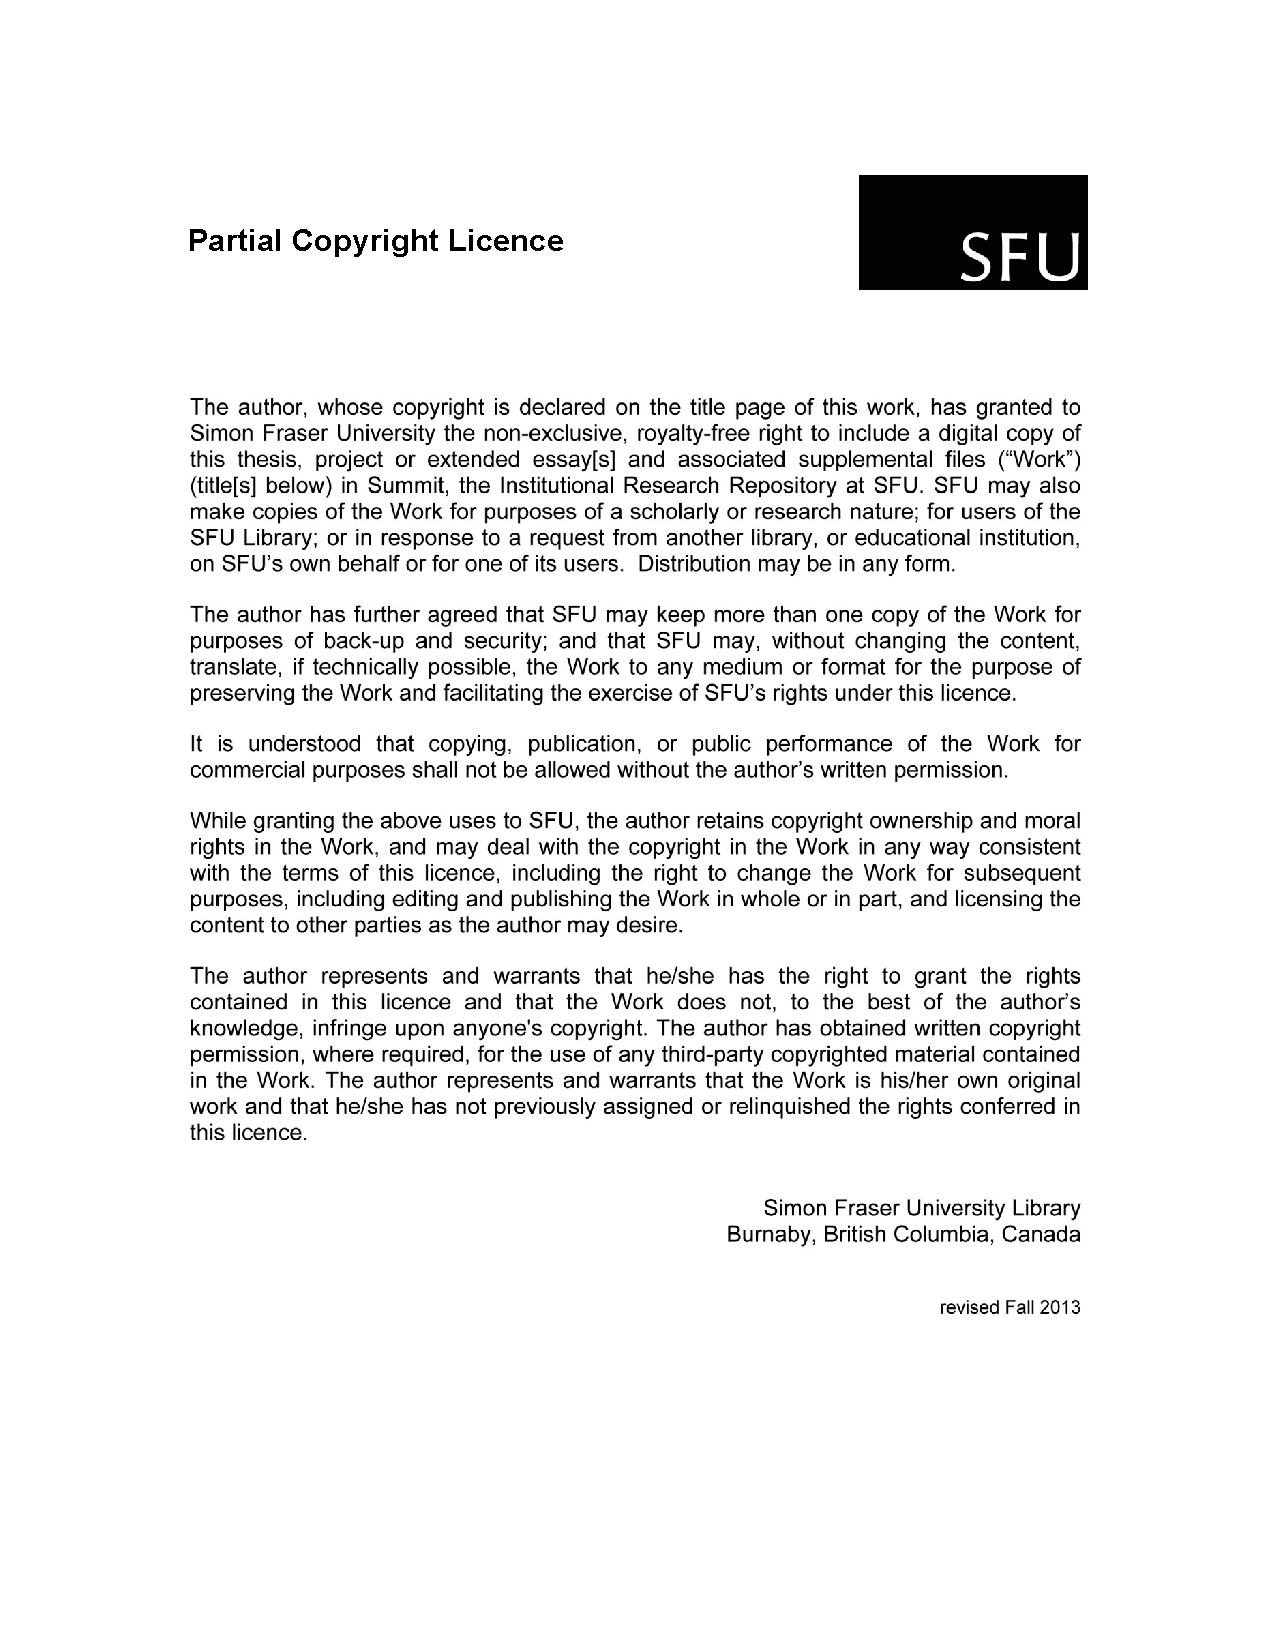
\includepdf[pagecommand={\thispagestyle{plain}}, pages={1}]
  {./0_frontmatter/partial-copyright.pdf}

% Abstract
%%%%%%%%%%%%%%%%%%%%%%%%%%%%%%%%%%%%%%%%%%%%%%%%%%%%%%%%%%%%%%%%%%%%%%%%%%%%%%%%
% PHD DISSERTATION ABSTRACT
%
%
% Michael Malick
% 2016-12-11
%
%%%%%%%%%%%%%%%%%%%%%%%%%%%%%%%%%%%%%%%%%%%%%%%%%%%%%%%%%%%%%%%%%%%%%%%%%%%%%%%%


\chapter*{Abstract}
\addcontentsline{toc}{chapter}{Abstract}

Environmental change resulting from natural or anthropogenic forcing can have
profound impacts on the structure and function of marine and coastal ecosystems.
Yet, determining environmental processes governing population dynamics of marine
and anadromous fish species remains an elusive problem that has practical
management implications. In this thesis, I use a cross-system comparative
approach to examine environmental forcing pathways linking climatic and ocean
processes to dynamics of Pacific salmon (\textit{Oncorhynchus} spp.) populations
in the Northeast Pacific Ocean. I begin by assessing the evidence for
population-level responses to inter-annual changes in two meso-scale ocean
processes, phytoplankton dynamics and ocean currents, which represent critical
links within two alternative sets of environmental forcing pathways. In the
first set of pathways, vertical ocean transport and subsequent phytoplankton
dynamics are hypothesized to mediate the effects of climate variability on
higher-trophic-level species, whereas in the second set of pathways, climate
effects are hypothesized to be mediated by horizontal ocean transport and
subsequent advection of plankton into coastal areas. I show that both
phytoplankton dynamics and ocean current patterns are strongly associated with
changes in salmon productivity, indicating that both sets of hypothesized
pathways may drive salmon dynamics. However, the magnitude and direction of the
effects were conditional on the latitude of juvenile salmon ocean entry,
suggesting that the relative importance of different environmental pathways may
be region dependent. Next, I use a novel quantitative method, probabilistic
networks, to examine the joint effect and relative strength of 17 potential
environmental pathways linking large-scale climate processes to Pacific salmon
dynamics. I show that multiple environmental pathways can simultaneously impact
salmon population dynamics, including multiple pathways originating from the
same climatic process. Finally, I use a policy perspective to examine how
challenges arising from a highly migratory life history can impede efforts to
integrate Pacific salmon into ecosystem-based management policies. My findings
indicate that ecosystem-based management policies should explicitly account for
mismatches in the scale at which ecosystem services are provided by highly
migratory species and the scale at which human activities and natural processes
impact those services to achieve more effective integration. Collectively, my
thesis demonstrates that climatic and ocean processes can impact
higher-trophic-level species via multiple simultaneously operating environmental
pathways and accounting for spatial heterogeneity in the relative importance of
these pathways may be critical to developing effective management strategies
that are robust to future environmental change.
\newline

\noindent \textbf{Keywords:} Pacific salmon; population dynamics; environmental
change; spatial non-stationarity; ecosystem-based management; productivity


\clearpage

% Quote
%%%%%%%%%%%%%%%%%%%%%%%%%%%%%%%%%%%%%%%%%%%%%%%%%%%%%%%%%%%%%%%%%%%%%%%%%%%%%%%%
% PHD DISSERTATION ABSTRACT
%
%
% Michael Malick
% 10 Feb 2015  
%
%%%%%%%%%%%%%%%%%%%%%%%%%%%%%%%%%%%%%%%%%%%%%%%%%%%%%%%%%%%%%%%%%%%%%%%%%%%%%%%%



\vspace*{7cm}

\begin{flushright}

\emph{``Everything should be made as simple as possible, but not simpler''} \\
\emph{-- Albert Einstein}

\vspace*{2cm}

\emph{``If I have seen farther it is by standing on the shoulders of giants''} \\
\emph{-- Sir Isaac Newton}

\end{flushright}

\clearpage

% Acknowledgements
% PHD THESIS ACKNOWLEDGEMENTS
% Michael Malick
% 2016-12-16


\chapter*{Acknowledgements}
\addcontentsline{toc}{chapter}{Acknowledgements}

I sincerely thank my supervisors Randall Peterman and Sean Cox for their
guidance, advice, and encouragement. My success reflects their ability as
mentors and I am grateful for their willingness to allow me the freedom to
explore new paths. To Randall, you provided an exceptional example of how to be
a great scientist and I will always be grateful for the opportunities you
provided me at SFU. To Sean, you have been a source of inspiration as a
scientist and I am grateful for you welcoming me into your lab.

I have benefited greatly from the advice and many insightful discussion with my
supervisory committee. I am grateful to Franz Mueter for being available to
discuss my research and taking the time to provide critical feedback. I thank
Murray Rutherford for his patience and guidance as I learned the details of
policy research and his clear and reliable insights into the policy process.

I am grateful to the individuals who participated as collaborators in my
research. Thanks to Thomas Wainwright and Bill Peterson, who hosted me in
Newport, OR, and provided keen insights into the Oregon Coast marine ecosystem.
I also thank Nathan Mantua and Todd Mitchell who hosted me at the University of
Washington and taught me the details of working with satellite data sets.

To my fellow lab members in the fisheries group at SFU, thank you for providing
me a source of companionship and your willingness and enthusiasm to discuss
anything quantitative. I am grateful to my colleagues in the REM PhD program who
provided inspiration and a sounding board for me to discuss my research.

I thank the many biologists from the Washington Department of Fish and Wildlife,
Fisheries and Ocean Canada, the Alaska Department of Fish and Game, and the
Newport Research Station for collecting and providing me with the numerous data
sets analyzed here. Without their efforts, this research would not have been
possible.

I am grateful for funding from the Canada Research Chairs Program provided to
Randall Peterman and for the numerous scholarships and fellowships provided by
Simon Fraser University that helped support my research.

It is beyond my abilities to thank my family for their encouragement during my
education. To my beautiful wife Erin, thank you for providing me a source of joy
and happiness everyday and your willingness to listen to me discuss the details
of my research. To my parents, brother, and extended family, thank you for your
unwavering support through all my years of education. Mother and Dad, you have
always given me the freedom to pursue my interests and provided me with
unconditional encouragement, thank you.

My life has be greatly enriched by these individuals, and for that I am
grateful.



\clearpage

% TOC
\phantomsection
\addcontentsline{toc}{chapter}{Contents}
\tableofcontents
\clearpage

% List of tables
\phantomsection
\addcontentsline{toc}{chapter}{List of Tables}
\listoftables
\clearpage

% List of figures
\phantomsection
\addcontentsline{toc}{chapter}{List of Figures}
\listoffigures
\clearpage
\pagenumbering{arabic}
\setcounter{page}{1} 

%%%%%

% Fancy Headers
\fancyhf{}
\renewcommand{\headrulewidth}{0pt} % remove header rule
\pagestyle{fancy}
\lhead{\small \textit{\leftmark}}
\rhead{\small \thepage}
% \pagestyle{headings} % default latex header


% Introduction
% General Introduction
% Michael Malick
% 2016-12-11

\chapter[General introduction]{General introduction}
\label{ch:intro}

Environmental forcing can have profound impacts on the provisioning of ecosystem
services generated by marine and coastal ecosystems. Yet, deep uncertainties
about the coupling among climate systems, physical and biological ocean
processes, and productivity\footnotemark[1] of higher-trophic-level species
limits our ability to anticipate or quickly detect impacts of changing
environmental conditions on commercially valuable species. These uncertainties
contribute to risks that have implications for conservation, harvest management,
and users of living marine resources. Effectively reducing uncertainties about
the links among different ecosystem components requires a quantitative
understanding about how perturbations in large-scale climatic and atmospheric
conditions propagate to regional and local scale changes in the population
dynamics of exploited species. In this thesis, I aim to add to that quantitative
understanding by applying a cross-system comparative approach to examine
environmental forcing pathways linking climatic and ocean processes to dynamics
of Pacific salmon (\emph{Oncorhynchus} spp.) populations in the Northeast
Pacific Ocean.

\footnotetext[1]{Throughout this thesis, the term productivity refers to the per
  capita growth rate for a population. For Pacific salmon, productivity is
  estimated as the number of recruits produced per spawner.}


\section{Large-scale environmental change}

Environmental change in marine and coastal ecosystems can arise from
anthropogenic sources or natural environmental stochasticity and can manifest as
gradual or abrupt changes in mean conditions or changes in the frequency or
distribution of extreme events \citep{Jentsch2007}. For example, gradual changes
in climate systems over the past five decades due to increased carbon dioxide
concentrations in the atmosphere have resulted in warmer mean atmosphere and
ocean temperatures, decreased snow and ice pack, rising sea levels, changes in
precipitation patterns, increased ocean acidification, and increased frequency
of extreme temperature events \citep{IPCC2013a}. The inter-decadal rate of
change for many of these abiotic ecosystem components is unprecedented with
equally rapid changes also being observed for biological processes including
shifts in phenology, species distributions, and fish stock productivity
\citep{IPCC2013a, Taylor2008a, Pinsky2013, Peterman2012}.

Concurrent with climate and ecosystem changes from anthropogenic forcing are
changes resulting from natural climate variability. In the Northeast Pacific,
large-scale climate patterns, e.g., the Pacific Decadal Oscillation and North
Pacific Gyre Oscillation, at least partially control the dynamics of marine and
coastal ecosystems. Fluctuations in these patterns, often referred to as regime
shifts, can substantially alter the structure and function of ecosystems that
comprise the Northeast Pacific \citep{Chavez2003a}. For instance, a rapid
ecological shift occurred in the Northeast Pacific in response to a climatic
regime shift in 1976/1977 (i.e., the Pacific Decadal Oscillation shifted from a
``cool regime'' to a ``warm regime''), which resulted in a taxonomic
reorganization in the Northeast Pacific where the abundances of wild adult
sockeye salmon (\emph{O. nerka}) and pink salmon (\emph{O. gorbuscha}) increased
by more than 65\% \citep{Ruggerone2010a, Anderson1999a, Mueter2000a}.

For Pacific salmon, effects of environmental change due to perturbations in
large-scale climatic conditions are mainly hypothesized to influence survival of
pre-recruit life stages. In particular, the first year of marine residency for
Pacific salmon is considered a critical period, i.e., mortality during this
life-stage can have a disproportionately large affect on overall stock
productivity compared to other life-stages \citep{Parker1968a, Peterman1985a,
Beamish2001a, Wertheimer2007a}. Although both bottom-up\footnotemark[2] and
top-down\footnotemark[3] forcing likely contribute to mortality during this
critical period, two pieces of evidence suggest that processes controlling food
resource availability are particularly important. First, juvenile salmon
mortality during the early marine life-stage is size selective, with larger
juveniles tending to survive to adult life-stages in higher proportions than
smaller juvenile salmon \citep{Parker1971a, Holtby1990a, McGurk1996a,
Moss2005a}. Second, growth rates during the early marine life-stage are strongly
and positively associated with overall marine survival rates \citep{Cross2008a,
Duffy2011, Farley2007b}. Together, this evidence suggests that large-scale
climatic perturbations likely have a strong impact on Pacific salmon year class
strength through bottom-up forcing pathways \citep{Perry1996a, Armstrong2005a}.

\footnotetext[2]{The term `bottom-up forcing' is used throughout this thesis to
  describe regulation of ecosystem structure and function through processes that
  affect the base of the food chain, such as nutrient supply and primary
  production.}

\footnotetext[3]{The term `top-up forcing' is used throughout this thesis to
  describe regulation of ecosystem structure and function occurring through
  predation.}


\section{Environmental forcing pathways}

A prevailing bottom-up forcing pathway in marine ecosystems posits that vertical
transport processes mediate the effects of climate variability on phytoplankton
dynamics in coastal ecosystems and subsequently, food resource availability for
juvenile Pacific salmon (Fig. \ref{fig:intro:1}) \citep{DiLorenzo2013b,
Rykaczewski2008a, Ware1991a}. In particular, atmospheric and ocean processes
controlling water column stability and the near surface nutrient supply are
frequently cited as key elements driving phytoplankton dynamics in coastal
Northeast Pacific ecosystems \citep{Henson2007a, Gargett1997a}. For example, in
coastal upwelling areas, winds drive surface waters offshore through Ekman
dynamics, causing nutrient rich subsurface water to upwell into the euphotic
zone, providing necessary nutrients for primary production \citep{Huyer1983}. In
turn, this primary production provides grazing opportunities for copepods and
other zooplankton, which are a critical food resource for juvenile Pacific
salmon during their early marine residency \citep{Armstrong2008a,
Beauchamp2007a, Brodeur2007a}. Over the past two decades, considerable evidence
has indicated strong connections between climate variability, vertical ocean
transport processes, and phytoplankton dynamics \citep{Chenillat2012,
Polovina1995a, Henson2007a, Henson2007b, Stabeno2004a, Weingartner2002a}.
However, relationships between lower-trophic-level process (e.g., phytoplankton
dynamics in coastal ecosystems) and productivity of Pacific salmon populations
largely remain untested assumptions. In chapter \ref{ch:bloom}, I investigate
the vertical transport hypothesis by asking whether the phenology or intensity
of the spring phytoplankton bloom can explain variability in productivity of 27
North American pink salmon stocks.

\begin{figure}[htbp]
  \centering
  \includegraphics[scale=0.4]{1_introduction/figures/vertical-horizontal.pdf}
  \caption[Schematic of two environmental forcing pathways.]{Schematic of two
           environmental forcing pathways linking large-scale climate patterns,
           ocean processes, and higher-trophic-level species.}
  \label{fig:intro:1}
\end{figure}

Recently, evidence for an alternative bottom-up forcing pathway has emerged,
suggesting that horizontal ocean transport may be equally important as vertical
transport in mediating the effects of climate variability on
higher-trophic-level species \citep{DiLorenzo2013b}. This horizontal transport
hypothesis proposes that food resources available to juvenile salmon in coastal
ecosystems is driven by climate-induced changes in horizontal transport
processes, e.g., ocean currents or eddies, that cause zooplankton or other
weakly/passive drifters to be advected into or out of coastal areas (Fig.
\ref{fig:intro:1}). For example, off the central Oregon Coast, research has
indicated that the negative phase of the Pacific Decadal Oscillation is
associated with increased advection of large-bodied lipid-rich zooplankton into
the region from northern areas, which in turn is associated with increased
marine survival of coho salmon (\emph{O. kisutch}) \citep{Keister2011a,
Bi2011a}. Beyond the Northern California Current area, however, the effects of
variability in horizontal ocean transport on Pacific salmon productivity are
largely untested. In chapter \ref{ch:npc}, I investigate the horizontal
transport hypothesis by examining the effects of two modes of variability in
horizontal ocean transport in the Northeast Pacific on productivity of 163 North
American pink, chum (\emph{O. keta}), and sockeye salmon stocks.

Although the vertical and horizontal transport pathways are individually
appealing to explain how climate forcing downscales to affect regional and local
scale dynamics of higher-trophic-level species, these hypotheses are not
mutually exclusive and may have additive or multiplicative effects on salmon
productivity. In particular, regional-scale vertical and horizontal transport
processes are both hypothesized to mediate the effects of large-scale climate
variability on lower- and higher-trophic-level species. Thus, perturbations to
climatic systems from anthropogenic or natural sources may simultaneously
influence regional-scale vertical and horizontal transport pathways. Indeed, the
Pacific Decadal Oscillation has been shown to influence ocean current patterns
in the Northern California Current ecosystem and affect the magnitude of
upwelling-favorable winds in the region \citep{Keister2011a, Chhak2007}.
Estimating the cumulative effects and relative importance of these
simultaneously operating pathways is likely a necessary component of
understanding how environmental change impacts higher-trophic-level species. In
chapter \ref{ch:bn}, I use a novel quantitative method, probabilistic
networks, to estimate the cumulative effects of these different pathways on
productivity of coho salmon in the Northern California Current.


\section{Managing for environmental change}

A better understanding of how environmental forcing impacts salmon populations
is a necessary but not sufficient condition for maintaining viable and
productive salmon stocks. We also need to develop a parallel understanding of
how these impacts interact with other anthropogenic disturbances, such as
commercial harvesting, and how this information can be incorporated into
management decisions \citep{Link2002a}. Increasingly, management of living
marine resources is moving toward ecosystem-based approaches to management that
shift the focus of management from a single-species to maintaining critical
components of ecosystem structure and function \citep{Grumbine1994,
Murawski2007a, Long2015}. A necessary element of this shift toward
ecosystem-based management is defining boundaries that delimit the spatial
extent of the decision-making process \citep{Engler2015, Yaffee1999}. However,
for highly migratory marine and anadromous fish species, impacts from human or
natural sources can occur across a continuum of spatial scales that frequently
extend beyond the boundaries of the ecosystem-based management area
\citep{Dallimer2015}. For example, management actions in locations that are
geographically distance from the ecosystem-based management area, such as
decisions to increase commercial harvests, may strongly impact the supply of
ecosystem services provided by a migratory species within the bounds of the
ecosystem-based management area. In chapter \ref{ch:ebm}, I examine challenges
associated with integrating highly migratory Pacific salmon into regional and
local scale ecosystem-based management policies that arise from mismatches
between the scale of management and the biology of Pacific salmon and discuss
potential strategies to overcome the identified challenges.


\section{Statement of interdisciplinarity}

The research presented in this thesis includes two levels of
interdisciplinarity. First is the incorporation of research ideas, perspectives,
and approaches from both oceanography and fisheries. Although both fields are
firmly rooted in the natural sciences, the research approaches and the types of
questions important to researchers in both fields have diverged over time
\citep{Platt2007a}. In chapters \ref{ch:bloom}--\ref{ch:bn}, I attempt to
bring together some of the knowledge and research questions important to both
fisheries scientists and oceanographers. The second level of interdisciplinarity
involves a bridge between the natural and social sciences. One-quarter of the
research presented in this thesis is focused on this bridging by taking a policy
perspective in order to answer an important fisheries question.


\section{Contributions}

I am the sole author of the general introduction and summary and conclusions and
these chapters are written in the first-person singular. Chapters
\ref{ch:bloom}--\ref{ch:ebm} are derived from either published manuscripts
or submitted manuscripts with co-authors and these chapters are written in the
first-person plural. For each of the chapters deriving from multi-authored
manuscripts (chapters \ref{ch:bloom}--\ref{ch:ebm}), I am the first-author
of the work and performed the data analysis and wrote the first draft of the
text. These chapters, however, benefited greatly from discussions, editing, and
comments from the co-author. The original published sources of these chapters
are provided at the beginning of each chapter. The initial ideas for chapter
\ref{ch:bloom} were developed by myself, Randall Peterman, Franz Mueter and
Sean Cox. Chapter \ref{ch:npc} builds on ideas originally presented in an
unpublished manuscript by Randall Peterman, Franz Mueter, and Brigitte Dorner.
The main idea for chapter \ref{ch:bn} came out of discussions between myself
and Randall Peterman following a presentation on using Bayesian networks for
ecological research by Catherine Michielsens. The ideas presented in chapter
\ref{ch:ebm} were developed by myself, Murray Rutherford, and Sean Cox.


\clearpage

% Spring-bloom
% Thesis Spring Bloom Chapter
% Michael Malick
% 2015-10-12

% \chapter[Phytoplankton phenology and salmon productivity]
\chapter[Phytoplankton phenology and salmon productivity]{Linking
  phytoplankton phenology to salmon productivity along a north-south gradient in
  the Northeast Pacific Ocean\footnotemark[1]}

\footnotetext[1]{A version of this chapter appears as 
  Malick, M.J., S.P. Cox, F.J. Mueter, R.M. Peterman. 2015. Linking
  phytoplankton phenology to salmon productivity along a north-south gradient in
  the Northeast Pacific Ocean. Canadian Journal of Fisheries and Aquatic
  Sciences 72:697-708. \url{http://doi.org/10.1139/cjfas-2014-0298}.}
  

\section{Abstract}

We investigated spatial and temporal components of phytoplankton dynamics in the
Northeast Pacific Ocean to better understand the mechanisms linking biological
oceanographic conditions to productivity of 27 pink salmon (\emph{Oncorhynchus
gorbuscha}) stocks. Specifically, we used spatial covariance functions in
combination with multi-stock spawner-recruit analyses to model relationships
among satellite-derived chlorophyll-a concentrations, initiation date of the
spring phytoplankton bloom, and salmon productivity. For all variables, positive
spatial covariation was strongest at the regional scale (0-800 km) with no
covariation beyond 1500 km. Spring bloom timing was significantly correlated
with salmon productivity for both northern (Alaska) and southern (British
Columbia) populations, although the correlations were opposite in sign. An early
spring bloom was associated with higher productivity for northern populations
and lower productivity for southern populations. Furthermore, the spring bloom
initiation date was always a better predictor of salmon productivity than mean
chlorophyll-a concentration. Our results suggest that changes in spring bloom
timing resulting from natural climate variability or anthropogenic climate
change could potentially cause latitudinal shifts in salmon productivity.



\section{Introduction}

The dynamics of marine fish populations are often characterized by large
inter-annual and inter-decadal variability in abundances. For Pacific salmon
(\emph{Oncorhynchus} spp.), the first year of ocean residence is widely viewed
as a critical period that can strongly influence stock abundance
\citep{Peterman1985a, Parker1968a, Wertheimer2007a}. During this period,
climatic and oceanographic conditions are believed to strongly affect salmon
productivity (i.e., the number of adult recruits produced per spawner), yet the
ecological pathways connecting environmental variability to upper trophic levels
of marine food webs are not well understood \citep{Drinkwater2010a,
Ottersen2010a}. Evidence suggests that salmon mortality during the early marine
life stage is inversely related to body size, indicating that bottom-up forcing
mechanisms that affect prey resources may be an important part of these
ecological pathways \citep{McGurk1996a, Duffy2011, Farley2007b}.

Several bottom-up forcing mechanisms have been proposed to explain productivity
variation in marine fish stocks, including salmon \citep{Cushing1990a,
Gargett1997a}. For example, the ``optimal stability window'' hypothesis suggests
that changes in water column stability may be a critical component linking
changes in large-scale climate patterns and salmon productivity
\citep{Gargett1997a}. However, this hypothesis assumes a strong link between
phytoplankton dynamics (e.g., productivity or total biomass) and salmon
productivity, which is largely untested beyond a few local-scale studies
\citep{Mathews1989a, Chittenden2010a}.  Accounting for both spatial and temporal
variability of lower-trophic-level processes is a key challenge to testing the
optimal stability window hypothesis on large spatial scales.

In the coastal Northeast Pacific, seasonal biomass of phytoplankton follows a
well-known pattern defined primarily by the spring bloom \citep{Henson2007a,
Waite2013}, which is mainly driven by large-scale climate patterns combined with
regional and local-scale physical environmental conditions \citep{Sverdrup1953a,
Ware1991a, Polovina1995a, Henson2007a}. In the coastal Gulf of Alaska, the
spring bloom initiation date is strongly correlated with the onset of water
column stability, which is at least partially controlled by the strength of the
Aleutian Low Pressure system \citep{Henson2007a}. In that region, an earlier
spring bloom is also associated with a more intense bloom, suggesting that both
the phenology of the spring bloom and overall production during the bloom may be
important components of bottom-up forcing pathways. Indeed, features of the
spring bloom such as initiation date and total phytoplankton biomass are
correlated with yield and productivity of certain marine fish populations
\citep{Platt2003a, Ware2005a, Koeller2009}.

In this paper, we asked whether the spring bloom initiation date and average
chlorophyll-a (chl-a) concentrations (a surrogate for phytoplankton biomass) can
explain spatial and inter-annual variability in pink salmon (\emph{O.
gorbuscha}) productivity, which we estimated using spawner-recruit data for 27
stocks. Establishing a plausible mechanistic link between the spring
phytoplankton bloom and salmon production first requires evidence that the two
processes operate at similar spatial scales; that is, spatial covariation of
lower-trophic level processes should approximately match the spatial scale of
covariation observed in the salmon productivity data that they are being used to
explain \citep{Bjornstad1999a, Koenig1999a}. In the Northeast Pacific Ocean,
productivity of salmon stocks exhibit spatial synchrony at the scale of 100 to
1000 km \citep{Mueter2002b} with positive correlations being greatest at
distances less than 500 km \citep{Pyper2005a}. Therefore, we hypothesized that
features of the spring phytoplankton bloom operate at similar regional spatial
scales as salmon productivity.

We used spatial covariance analyses to determine the spatial extent of synchrony
in the timing of the spring phytoplankton bloom and mean chl-a concentrations
along the Northeast Pacific coast, as well as to determine the scale of spatial
averaging that should be used on data for these variables. We then used a
hierarchical, multi-stock statistical modeling approach to estimate
relationships between pink salmon productivity and inter-annual variability in
spring bloom initiation date, as well as mean chl-a concentration during spring
and late summer.  Compared to single-stock analyses, our multi-stock modeling
approach can help reduce uncertainty associated with the biological processes
that underpin the dynamics of salmon populations and reduce the chance of
finding spurious relationships by using different salmon stocks as replicates
within the analysis \citep{Myers1998c, Myers1999a}.



\section{Methods}

\subsection{Pink salmon data}

We estimated annual indices of productivity (in units of adult recruits per
spawner) for 27 wild pink salmon stocks from British Columbia (B.C.) and Alaska
(AK) using data on spawner abundance and total recruitment (catch plus
escapement). The 27 spawner-recruit data sets (Table \ref{tab:bloom:1})
represent aggregations of escapement and catch of adjacent salmon stocks. The
aggregation helped ensure that catches were attributed to the correct spawning
stocks and was primarily based on jurisdictional management units, although in
some cases aggregation occurred at a larger scale because of difficulty
allocating catch into individual management units (e.g., Prince William Sound).
Hatchery returns were excluded from all estimates of catch and escapement.
Estimation methods for spawner abundances varied among stocks, but in general,
southern stocks (B.C.) were estimated using expansions of foot surveys, while
northern stocks (AK) were estimated using expansions of aerial surveys (personal
communication from data sources listed in footnotes of Table \ref{tab:bloom:1}).
Annual recruitment varied widely among stocks with long-term averages ranging
from 0.12 million pink salmon for Chignik Bay to 33.31 million for southern
southeast Alaska (Table \ref{tab:bloom:1}).

\subsection{Chlorophyll-a data}

We used satellite-derived chl-a concentration estimates (measured as mg
m\textsuperscript{-3}) from the Sea-viewing Wide Field-of-view Sensor (SeaWiFS)
and the Moderate Resolution Imaging Spectroradiometer (MODIS-Aqua) from the
Goddard Space Flight Center (\url{http://oceancolor.gsfc.nasa.gov}). Level-3
processed data were downloaded for 1998-2010 (but only 2003-2010 had complete
MODIS data) in their original 9 km\textsuperscript{2}, 1-day-resolution. We
converted the data to a 1$^{\circ}$x1$^{\circ}$ resolution and subsetted the
resulting grid to 46$^{\circ}$--61$^{\circ}$N and 167$^{\circ}$--125$^{\circ}$W,
including only grid cells adjacent to the coast (Fig.  1). We excluded grid
cells in the Bering Sea because all salmon stocks in our data set enter the
ocean in the Gulf of Alaska.

All analyses were performed using 8-day composite chl-a data because these had
less missing data across all years compared to 1-day and 5-day composites
(Supporting materials Fig. \ref{fig:bloom:s1}). In addition, the SeaWiFS data
set had numerous large gaps during the spring and summer for years 2008-2010,
which made these years of SeaWiFS data unsuitable for our study (Supporting
materials Fig. \ref{fig:bloom:s1}). We evaluated the feasibility of
concatenating the SeaWiFS and MODIS data sets into a single continuous data set
that would provide an additional three years of data (compared to using SeaWiFS
data alone) by comparing the two data sets over the first five overlapping years
(2003-2007; Supporting materials \ref{supp:bloom:A}). We estimated correlations,
root mean squared log\textsubscript{10} error (RMSE), and log\textsubscript{10}
bias to quantify differences between the two chl-a data sets. The SeaWiFS and
MODIS data sets were highly correlated (average of 0.87 across all grid cells).
In addition, over all years and grid cells RMSE (0.16) and log bias (0.012)
(Supporting materials Fig. \ref{fig:bloom:s2}) were consistent with other
studies comparing SeaWiFS and MODIS data products over a similar study region
\citep{Waite2013}. Based on these minimal differences, we concatenated the
SeaWiFS (1998-2002) and MODIS (2003-2010) data sets without further processing.

Inter-annual variability in phytoplankton standing stock and phytoplankton
phenology were quantified using mean monthly chl-a concentration and the
spring-bloom initiation date, respectively, which we derived from the 8-day
composite chl-a estimates for each grid cell (Fig. \ref{fig:bloom:1}). We
linearly interpolated data points in chl-a time series for each grid cell
between gaps less than 3 data points (4.1\% of all chl-a data points were
interpolated). This procedure was done prior to estimating annual spring bloom
initiation date and mean chl-a concentrations. We estimated the spring bloom
initiation date as the first 8-day period in a given year when the chl-a
concentration was more than 5\% above the median chl-a concentration of the
entire multi-year data set for a particular grid cell \citep{Siegel2002a,
Henson2007a}. In addition, we log\textsubscript{10}-transformed the chl-a
averages to help normalize the chl-a values.


\subsection{Spatial covariation analysis}

We constructed cross-correlation matrices to quantify spatial covariance
patterns for (1) pink salmon stock productivities, (2) spring-bloom initiation
dates, and (3) monthly mean chl-a concentrations. For salmon stocks, pairwise
correlation coefficients were computed between time series of productivity for
each of the 27 stocks. For the spring bloom initiation date, correlation
coefficients were computed between each pair of grid cells using time series of
the estimated annual spring bloom initiation date for years 1998-2010. For chl-a
concentration, we calculated correlations across grid cells using time series of
the monthly mean chl-a concentration. To account for potential changes in
spatial patterns across seasons, we calculated correlations for chl-a
concentration for each month (February-October) separately.

We estimated annual salmon productivity using residuals from a Ricker
spawner-recruit model, which removed potential within-stock density-dependent
effects \citep{Pyper2001a, Mueter2002a, Ricker1954a}.  The Ricker model for each
stock was of the form,

\begin{equation}
log_e(R_{i,t} / S_{i,t}) = \alpha_i + \beta_i S_{i,t} + \epsilon_{i,t},
\label{eq:bloom:1}
\end{equation}

\noindent where \(R_{i,t}\) is total pink salmon recruits for the \(i^{th}\)
stock in brood year \(t\), \(S_{i,t}\) is the spawning stock two years earlier,
\(\alpha_i\) is the maximum log\textsubscript{e} recruits-per-spawner,
\(\beta_i\) is the coefficient of density-dependence, and \(\epsilon_{i,t}\) is
the residual.

We fit the Ricker models (eq. \ref{eq:bloom:1}) to two partitions of the data --
one including all available brood years and the second including only brood
years 1997-2009 (Table \ref{tab:bloom:1}). The latter partition corresponds to
the years available for the bloom initiation date and chl-a variables. Because
juvenile pink salmon enter the ocean the year following spawning (i.e., brood
year + 1), we offset the phytoplankton variables one year to correspond with the
ocean entry year for pink salmon (e.g., 2006 brood year was lined up with 2007
phytoplankton variables).

To test whether spatial covariation was present in each of the variables, we
first performed Mantel tests using matrices of the cross-correlations and a
matrix of great-circle distance (computed using the haversine formula) between
all pairs of grid cells or stocks \citep{Legendre1998a, Koenig1999a}.
Statistical significance of Mantel statistics were determined using
randomization tests with 1 000 permutations. We then determined the spatial
scale of covariation for each significant Mantel test by fitting a smooth
non-parametric covariance function \citep{Bjornstad2001a} between the
correlation coefficients for a given variable and the distance separating
correlated grid cells or ocean-entry points of salmon stocks. Confidence
intervals (CI) for each covariance function were computed by bootstrapping the
estimation procedure 1 000 times.

Covariance functions were summarized using two distance metrics: (1) the
y-intercept of the covariance function, which provides an estimate of the
correlation at zero distance (CZD), and (2) 50\% correlation scale (D50). The
CZD was estimated by extrapolating the fitted covariance function to zero
distance to find the y-axis intercept. The D50 was estimated as the distance at
which the covariance function falls to 50\% of its observed maximum value, which
provides a useful metric of how much the correlation declines with increasing
distance between salmon stocks or grid cells \citep{Mueter2002b}.


\subsection{Salmon productivity models}

We used a combination of single-stock linear models and multi-stock linear
mixed-effects models to investigate relationships among temporal averages of
mean chl-a concentrations (spring and late summer), spring bloom initiation
date, and pink salmon productivity. The single-stock model analysis had two
purposes. First, we used the values of fitted coefficients for different stocks
to inform construction of the multi-stock models and to help evaluate the
multi-stock model assumptions. Second, we used the single-stock analysis along
with intervention analyses to break up the data sets spatially to provide the
best fits of the multi-stock models. For both single-stock and multi-stock
models, only pink salmon brood years 1997-2009 were used.

The bloom initiation date and both chl-a covariates included in the models
represented spatial and temporal (for chl-a) averages of conditions experienced
by juvenile pink salmon during their early marine life phase. The bloom
initiation covariate was calculated for each salmon stock as the average of grid
cell specific anomalies (i.e., a grid cell's value minus the long term mean for
that grid cell) over all grid cells whose centers were within 250 km of the
stock's ocean entry point. For chl-a, we calculated April-May averages to
capture variability in phytoplankton biomass during the spring bloom and
July-September averages to index chl-a variability during the late summer, which
is believed to be a critical period for juvenile salmon survival
\citep{Beamish2001a, Moss2005a}. For both time periods, we first averaged chl-a
values over the specified months for each grid cell and then averaged over all
grid cells within 250 km of the stock's ocean entry point.


\subsubsection{Single-stock models}

The single-stock Ricker models took the form \citep{Adkison1996b},

\begin{equation}
log_e(R_{i,t} / S_{i,t}) = \alpha_i + \beta_i S_{i,t} + \gamma_i
X_{i,t+1} + \epsilon_{i,t}, \label{eq:bloom:2}
\end{equation}

\noindent where \(S_{i,t}\) is spawner abundance of pink salmon in brood year
\(t\) for the \(i^{th}\) stock, \(R_{i,t}\) is the total recruitment resulting
from \(S_{i,t}\), \(\alpha_i\) indicates stock productivity at low spawner
abundances, \(\beta_i\) indicates the magnitude of density-dependence,
\(X_{i,t+1}\) is a stock-specific measure of either the spring bloom initiation
date or mean chl-a concentration (the latter for either the spring or late
summer), \(\gamma_i\) is the coefficient for either the stock-specific bloom
initiation date or mean chl-a, and \(\epsilon_{i,t} \sim N(0, \sigma^2)\) is an
independent and identically distributed residual term.

Environmental variables such as sea surface temperature could have opposite
effects on northern and southern pink salmon stocks \citep{Mueter2002a,
Su2004a}; therefore we used an intervention model with two means
\citep{Chatfield2004, Mueter2002a} to test for differences in the effect of the
bloom initiation date and chl-a concentration between northern and southern
stocks \citep{Chatfield2004, Mueter2002a}. The intervention models were fit to
either the estimated chl-a or spring bloom coefficients from the single-stock
models (i.e., \(\gamma\) in eq. \ref{eq:bloom:2}) where the coefficients were
arranged south to north based on ocean entry locations (i.e., by stock number in
Table \ref{tab:bloom:1}).


\subsubsection{Multi-stock models}

We used hierarchical, multi-stock models to estimate both regional and
stock-specific effects of spring and late summer chl-a and the bloom initiation
date on pink salmon productivity, while also accounting for heterogeneity in
density-dependence among stocks. The multi-stock mixed effects Ricker models
took the form \citep{Myers1999a, Mueter2002a},

\begin{equation}
log_e(R_{i,t}/S_{i,t}) = \alpha + a_i - \beta_iS_{i,t} + 
X_{i,t+1} (\gamma_{X} + g_{i}) + \epsilon_{i,t}, \label{eq:bloom:3}
\end{equation}

\noindent where the fixed intercept \(\alpha\) is the overall mean productivity
common to all stocks and \(a_i\) is the stock-specific deviation from that mean,
\(\beta_i\) is the fixed stock-specific density-dependent effect, \(X_{i,t+1}\)
represents either the spring bloom initiation date or mean chl-a concentration
(either spring or late summer average), \(\gamma_X\) is the overall mean effect
of either the spring bloom initiation date or mean chl-a concentration, \(g_i\)
is the stock-specific deviation from that overall mean for a particular chl-a
variable, and \(\epsilon_{i,t}\) is an independent and identically distributed
residual term (i.e., \(\epsilon_{i,t} \sim N(0,\sigma^2)\)).  The stock-specific
random effects \(a_i\) and \(g_i\) are assumed to follow a joint normal
distribution with means zero, variances \(\sigma^2_a\) and \(\sigma^2_g\), and
covariance \(\sigma^2_{ag}\).

Because the chl-a and bloom initiation variables were moderately correlated
(average correlations between stock-specific phytoplankton time series ranged
from -0.50 to 0.20), the multi-stock models were fit separately for the bloom
initiation date and both chl-a metrics. For the bloom initiation date and spring
chl-a variables, we also fit multi-stock models separately for a southern stock
group (stocks 1-9 in Table \ref{tab:bloom:1}) and a northern stock group (stocks
10-27 in Table \ref{tab:bloom:1}), because the single-stock analysis and
intervention models suggested consistent differences in the effects of these
variables between northern and southern stock groupings (see Results). For the
late summer chl-a variable, we fit a single model using all stocks because the
intervention models did not indicate a significant break between northern and
southern stock groupings.

In addition to the full models (eq. \ref{eq:bloom:3}) for both chl-a variables
and the bloom initiation date, we investigated two simpler nested models, (1)
eq. \ref{eq:bloom:3} but without the random chl-a or bloom effect (i.e.,
\(g_{i}\)), and (2) eq. \ref{eq:bloom:3} but without either the random or fixed
chl-a or bloom effect (i.e., \(g_{i}\) and \(\gamma_{X}\), which was the null
model).  Random effect significance was determined using likelihood ratio (L)
tests among the nested models, whereas fixed effect significance was tested
using F-tests \citep{Pinheiro2000a}. All reported parameters were estimated
using restricted maximum likelihood methods; however, for model comparisons,
parameters were estimated using maximum likelihood methods to reduce bias
\citep{Pinheiro2000a}.

To compare the relative importance of the bloom initiation date and both chl-a
variables, we also calculated the small-sample Akaike Information Criterion
(AIC\textsubscript{C}) for all models \citep{Hurvich1989a, Burnham2002a}. For
the models that included late summer chl-a, which were fit using all 27 salmon
stocks, we calculated a single set of AIC\textsubscript{C} values (one for each
nested model).  For the models that included either the bloom initiation date or
spring chl-a variables, we calculated two sets of AIC\textsubscript{C} values.
First, to compare the relative importance of both variables within the northern
and southern areas, we calculated AIC\textsubscript{C} values for each model fit
to the northern and southern stock groups separately.  Second, to compare
variable importance with the late summer chl-a variable, we calculated an
AIC\textsubscript{C} value for the combined northern and southern models.
Because northern and southern models for the bloom initiation date and spring
chl-a variables were fit using identical salmon data as the late summer chl-a
models, we calculated a combined northern and southern AIC\textsubscript{C}
value for each variable by summing the log-likelihoods and the number of model
parameters. To more easily compare models, we also calculated the
\(\Delta\)AIC\textsubscript{C}, i.e., the difference between each individual
model's AIC\textsubscript{C} value and the minimum AIC\textsubscript{C} value
among models. Models within three AIC\textsubscript{C} units of the model with
the lowest AIC\textsubscript{C} value are considered equally plausible
\citep{Burnham2002a}.


\subsection{Sensitivity analysis}

We checked the sensitivity of our results to four assumptions. First, we
estimated sensitivity of the spatial analysis results to an alternative
Beverton-Holt stock-recruitment model \citep{Beverton1957a} ($log_{e}(R/S) =
log_{e}(a) - log_{e}(1 + bS) + \epsilon$).  Second, we checked the sensitivity
to the interpolation procedure used on the chl-a time series by re-running each
analysis using spring bloom and chl-a values that did not include interpolated
data points. Third, we tested our assumption that the error terms of the
multi-stock models were temporally independent by refitting the models with
first-order autocorrelated errors (i.e., \(\epsilon_{i,t} = \phi\epsilon_{i,t-1}
+ \upsilon_t\), where \(\upsilon_t \sim N(0, \sigma^2)\)) and using likelihood
ratio tests to determine the significance. Fourth, because our spawner-recruit
data sets include variability associated with both freshwater and marine life
phases, we checked the sensitivity of our results to the source of pink salmon
data by comparing each chl-a metric to pink salmon marine survival rates for
three Alaska hatchery stocks (Armin F. Koernig, Kitoi Bay, and Port Armstrong)
using Pearson correlation coefficients (see Supporting materials
\ref{supp:bloom:B} for details of the analysis).



\section{Results}

\subsection{Spatial analysis}

Both sets of pink salmon residuals, monthly mean chl-a, and bloom initiation
date all showed significant spatial covariation (P \textless{} 0.01 for all
Mantel tests). For both sets of pink salmon residuals (all brood years and
recent, satellite-covered years), the nonparametric covariance functions
indicated declining positive covariation with increasing distance between ocean
entry points of juvenile salmon, up to approximately 800 to 1000 km where the
functions approached zero correlation (Fig. \ref{fig:bloom:2}a and b). The
estimated D50 was slightly larger for productivity indices fitted using all
available brood years (D50 = 305 km; 95\% CI = 218-488 km) than for indices
fitted using only brood years 1997-2009 (D50 = 261 km; 95\% CI = 148-628 km),
although there was considerable overlap in confidence intervals (Figs.
\ref{fig:bloom:2} and \ref{fig:bloom:3}a). Correlations at zero distance (i.e.,
the y-intercept of the covariance function) for both sets of productivity
indices were considerably less than one (CZD = 0.51; 95\% CI = 0.41-0.62 and CZD
= 0.49; 95\% CI = 0.28-0.69 for all brood years and 1997-2009 respectively; Fig.
\ref{fig:bloom:3}b). Although the nonparametric covariance function for bloom
initiation date had a slightly larger D50 (D50 = 367 km; 95\% CI = 235-776 km)
than the two salmon productivity indices, there was considerable overlap in
confidence intervals with both productivity indices (Fig. \ref{fig:bloom:3}a).
Correlation at zero distance for the bloom initiation date was also considerably
less than one (CZD = 0.44; 95\% CI = 0.33-0.55; Fig. \ref{fig:bloom:3}b).

For monthly mean chl-a concentrations, covariation decayed steeply with
increasing distance over spatial scales of 0-500 km for all months (Fig.
\ref{fig:bloom:4}).  The D50 was highest (\textasciitilde{}380 to 430 km) during
the winter and spring (February-May) and declined to about 250 km during summer
and fall (June-October), which was similar to the estimated D50 for salmon
productivity (Fig. \ref{fig:bloom:5}). In addition, confidence intervals for the
chl-a D50 for all months overlapped the confidence intervals for salmon
productivity D50s (Fig.  \ref{fig:bloom:5}). The CZD for chl-a concentrations
ranged from 0.56 in June to 0.76 in April, which was slightly higher than the
estimated CZD for the bloom initiation date and salmon productivity.


\subsection{Single-stock models}

The single-stock Ricker models indicated that pink salmon productivity was
related to the spring bloom initiation date either positively (15 stocks) or
negatively (12 stocks) (Fig. \ref{fig:bloom:6}a). The distribution of model
coefficients (i.e., \(\gamma\) in eq. \ref{eq:bloom:2}) ranged from -0.55 to
0.25 and was asymmetric about zero with the majority of values between -0.2 and
0.25 (Fig.  \ref{fig:bloom:6}d).  Productivity of all 9 pink salmon stocks south
of northern southeast Alaska (i.e., stocks 1-9 in Table \ref{tab:bloom:1}) was
positively related to the spring bloom initiation date, whereas productivity of
northern stocks was mostly negatively related (12 of 18 stocks; Fig.
\ref{fig:bloom:6}a). The intervention model indicated a significant break (P
\textless{} 0.05) in the sign of these relationships near 55.7$^{\circ}$N, which
was between the southern southeast Alaska stock (stock 9) and the northern
southeast Alaska outside stock (stock 10; Fig.  \ref{fig:bloom:1}).

Pink salmon productivity was also both positively (14 stocks) and negatively (13
stocks) related to spring chl-a concentrations (Fig. \ref{fig:bloom:6}b) with
the coefficients ranging from -3.4 to 6.0 (Fig. \ref{fig:bloom:6}e). Like the
bloom initiation date, the intervention model indicated a significant break (P
\textless{} 0.05) between stocks 9 and 10 for the spring chl-a coefficients
(Fig. \ref{fig:bloom:6}b). Productivity for all but two stocks in the southern
group had a negative relationship with spring chl-a concentrations, whereas the
northern group had a mix of positive and negative relationships.

For the late summer chl-a variable, productivity was consistently negatively
related to chl-a, with only 4 of the 27 stocks having a positive relationship
(Fig. \ref{fig:bloom:6}c). The coefficients were approximately normally
distributed with the magnitudes ranging from -8.6 to 3.2 with a median value of
-1.9 (Fig.  \ref{fig:bloom:6}f). In contrast to the other two phytoplankton
variables, the intervention model did not indicate a significant break in the
sign of the coefficients between northern and southern stocks (Fig.
\ref{fig:bloom:6}c).

The productivity parameters (\(\alpha\)) for the bloom initiation date and both
chl-a models were approximately normally distributed (a requirement for the
multi-stock models), but the distribution of the density-dependent coefficients
(\(\beta\)) had a long left tail (Supporting materials Fig. \ref{fig:bloom:s3}).


\subsection{Multi-stock models}

Over all pink salmon stocks we considered, productivity was significantly
related to spring bloom initiation date (northern and southern models), spring
chl-a concentrations (southern model only), and late summer chl-a (\(\gamma\) in
Table \ref{tab:bloom:2}), although stock-specific differences were not
significant in any models. For the bloom initiation date, regional effects were
opposite in sign for the northern and southern stock groups (\(\gamma\) in rows
2 and 5 in Table \ref{tab:bloom:2}, Fig. \ref{fig:bloom:6}a), suggesting that
salmon productivity for the southern stock group is higher than average when the
bloom is later (positive coefficient), whereas productivity is higher than
average for the northern stock group when the bloom is early (negative
coefficient). This result contrasts with those for spring (southern model only)
and late summer chl-a, where the regional effect was negative, implying reduced
salmon productivity when chl-a concentrations are higher (\(\gamma\) in rows 6
and 10 in Table \ref{tab:bloom:2}). Furthermore, the spring bloom initiation
date was a better predictor of salmon productivity than mean chl-a concentration
for all subsets of data (i.e., northern stock group, southern stock group, and
all stocks) (AIC\textsubscript{C} values in Table \ref{tab:bloom:2}).

Estimates of the regional effect of the spring bloom initiation date on salmon
productivity were significantly different than zero for both northern and
southern multi-stock models (\(\gamma\) in rows 2 and 5 in Table
\ref{tab:bloom:2}), but the models were not significantly different than the
full model (eq. \ref{eq:bloom:3}), which included both the regional and
stock-specific effects (L = 0.03, P \textgreater{} 0.1). The estimated
region-wide effect of spring chl-a concentrations on salmon productivity of
southern stocks and late summer chl-a on productivity of all stocks were
significantly different from zero (\(\gamma\) in rows 6 and 10 in Table
\ref{tab:bloom:2}). However, for both models and chl-a variables, there was no
evidence of stock-specific effects based on likelihood ratio tests comparing the
full models to a model without the random chl-a effects (L = 0.001, P
\textgreater{} 0.1 for both spring and late summer chl-a). In addition, for the
northern stock group there was no support for either a regional or
stock-specific effect of spring chl-a (row 3 in Table \ref{tab:bloom:2}; L =
0.001, P \textgreater{} 0.1).

In both the northern and southern areas, the bloom initiation date had a
stronger effect on pink salmon productivity than spring chl-a concentrations as
shown by the \(\Delta\)AIC\textsubscript{C} of 5.4 between the best fit models
for chl-a and the bloom initiation for the northern stock group and 12.5 for the
southern stock group (Table \ref{tab:bloom:2}).  The bloom initiation date also
had the highest relative importance (\(\Delta\)AIC\textsubscript{C} = 0) when
the northern and southern models were combined with an AIC\textsubscript{C}
value considerable less than late summer chl-a, spring chl-a, and the null model
(rows 7-10 in Table \ref{tab:bloom:2}). Between the two chl-a variables, the
late summer chl-a average had a higher relative importance (i.e., lower
AIC\textsubscript{C} value) than the average spring chl-a concentration as
indicated by the 10 unit difference between AIC\textsubscript{C} values (rows 9
and 10 in Table \ref{tab:bloom:2}).


\subsection{Sensitivity analysis}

Our estimates of the spatial covariation in pink salmon productivity were not
sensitive to the form of stock-recruit model because residuals from the Ricker
and Beverton-Holt models were highly correlated (average correlation across
stocks = 0.97). The D50 and CZD values were nearly identical between models fit
using the Ricker and Beverton-Holt residuals. Similarly, the spatial analyses
were not sensitive to the interpolation of data points in the chl-a time series.
Difference between D50 values for the interpolated and non-interpolated spring
bloom series was 10 km, with almost complete overlap of the confidence
intervals. In addition, changes in D50 for monthly chl-a without interpolation
values ranged from 0 km to 10 km across months with almost complete overlap of
the confidence intervals. Coefficients of the multi-stock Ricker model were also
insensitive to the interpolation of missing data.

The results from the multi-stock models were not sensitive to our initial
assumption of uncorrelated errors. Specifically, the single-stock models did not
indicate strongly autocorrelated errors, and adding an autocorrelated error term
to the best-fit multi-stock models did not significantly improve the fits for
any of the models, which is consistent with other research on pink salmon
productivity \citep{Pyper2001a}. In addition, comparisons between the three
chl-a metrics and hatchery marine survival rates broadly agreed with the results
of the multi-stock models (Supporting materials \ref{supp:bloom:B} and Fig.
\ref{fig:bloom:s4}).



\section{Discussion}

We investigated two indices of phytoplankton dynamics, spring bloom initiation
date and mean chl-a concentration, to better understand the potential mechanisms
linking biological oceanographic conditions to Pacific salmon productivity. Our
results indicated that (1) spatial covariation patterns for the spring bloom
initiation date, average chl-a concentration, and pink salmon productivity were
similar, with strongest positive covariation at the regional scale (0-800 km),
(2) there were opposing effects of the spring bloom initiation date on northern
and southern pink salmon stock productivity with an early bloom initiation date
being associated with higher northern stock productivity and a late bloom being
associated with higher southern stock productivity, (3) phytoplankton biomass
during the late summer (July-September) was more strongly associated with salmon
productivity than phytoplankton biomass during the spring (April-May), and (4)
the spring bloom initiation date was a better predictor of salmon productivity
than mean chl-a concentration for both southern and northern stocks.

Spatial synchrony for all three variables was strongest at regional spatial
scales and declined rapidly with increasing distance. For the bloom initiation
date and chl-a concentration, this suggests that physical processes operating on
relatively small spatial scales (e.g., summer sea surface temperature and sea
surface salinity) drives the spatial variability, rather than larger-scale
atmospheric processes such as the Pacific Decadal Oscillation
\citep{Mueter2002b}. For pink salmon productivity, our results suggest that both
phytoplankton biomass and the bloom initiation date could be factors driving the
regional-scale covariation. Furthermore, the match in spatial synchrony between
both phytoplankton variables and salmon productivity supports the inclusion of
these variables in the single-stock and multi-stock models and also lends
support for the observed correlations between pink salmon productivity and both
phytoplankton variables.

Spatial correlation of all three variables was less than one at zero distance,
indicating the presence of a ``nugget effect'', which represents variability due
to sampling error or spatial dependence at smaller scales than those sampled
\citep{Cressie1993}. For pink salmon productivity, this could be caused by
errors enumerating spawner abundances. For chl-a and the bloom initiation date,
the nugget effect may be caused by measurement errors in the chl-a estimates and
spatial averaging, or from the presence of small-scale oceanographic features
such as tidal mixing or river plumes that can lead to large changes in the bloom
initiation date and chl-a concentrations over short distances (\textless{} 100
km) \citep{Henson2007a}. The latter process could reduce the explanatory power
of both phytoplankton variables for salmon productivity because the
phytoplankton variables may not index conditions that salmon actually experience
at small spatial scales.

There was a marked reduction in the D50 for monthly chl-a concentrations between
May and June. The winter and spring period (February-May) included months with
both the highest annual chl-a concentrations (April and May) and the lowest
(February and March), whereas the chl-a concentrations during June-October were
relatively constant (Supporting materials Fig. \ref{fig:bloom:s5}). These
periods correspond to times before the spring bloom (February and March), during
it (April and May), and after it (June-October). Our results also showed that
coherence in chl-a concentrations following the spring bloom is smaller than
prior to and during the bloom, which may result from different mechanisms
underlying the spatial synchrony at different periods. For example, spatial
synchrony before and during the bloom may be primarily driven by regional-scale
physical oceanographic conditions such as sea surface temperature or sea surface
salinity \citep{Henson2007a}. In contrast, the period after the bloom also tends
to correspond to the period of peak zooplankton abundances in the Northeast
Pacific, indicating that chl-a concentrations after the bloom may be more
influenced by top-down grazing pressure, as suggested by others
\citep{Chittenden2010a, Bornhold2000, Mackas2012}.

A plausible explanation for the opposite effects of the bloom initiation date on
productivity of northern and southern stocks is that the spring bloom initiation
date is a surrogate for other processes that have direct effects on salmon
productivity such as predator abundances or zooplankton distributions. The
dividing line between the northern and southern stocks occurred in southern
southeast Alaska, which falls in the transition zone between the northern
downwelling domain and southern upwelling domain \citep{Ware1989a}. In the
northern region, the spring bloom initiation date has been shown to be closely
linked to the timing of water column stability, which is primarily determined by
freshwater runoff in the spring \citep{Weingartner2005a, Henson2007a}. Moreover,
both stability and the bloom initiation date in the northern domain tend to
occur earlier in warmer, wetter years that are associated with a more intense
Aleutian Low, higher zooplankton biomass, and increased salmon productivity
\citep{Brodeur1992a, Mueter2002a}. In the southern domain, an earlier spring
bloom is also associated with increased water column stability, however,
stability in this region is primarily driven by increased thermal warming and
reduced upwelling-favorable winds, both of which are also associated with a
stronger Aleutian Low \citep{Polovina1995a, Henson2007a}. In contrast to the
northern domain, these conditions in the south for an early bloom initiation
have been shown to be associated with increased predator abundances, reduced
zooplankton biomass, and decreased salmon productivity \citep{Ware1995a,
Mackas2001a, Mueter2002a}.

The optimal stability window hypothesis \citep{Cury1989a, Gargett1997a} provides
another possible explanation for the opposite effects of the bloom initiation
date on productivity of northern and southern stocks.  This bottom-up forcing
mechanism posits that synchronous changes in water column stability in northern
and southern areas, which are driven by strength of cyclonic circulation in the
Gulf of Alaska \citep{Gargett1997a}, can lead to out-of-phase salmon survival
rates between the two areas. However, the degree to which our results support
the optimal stability window hypothesis depends on the extent to which (1) water
column stability and the spring bloom initiation date are linked, (2) water
column stability has opposite effects on primary production in northern and
southern regions, and (3) there is a strong positive relationship between
phytoplankton biomass and salmon productivity. Although the first two
relationships are beyond the scope of this research, our results indicate that
there is only a weak relationship between phytoplankton biomass during the
spring and salmon productivity and a stronger but negative relationship between
phytoplankton biomass during the late summer and salmon productivity.

The latitudinal shift in the effect of the spring bloom initiation date on
northern and southern stock productivity corresponds with previous studies that
showed opposite effects of sea surface temperature on the productivity of
northern and southern pink salmon, chum salmon (\emph{O.  keta}), and sockeye
salmon (\emph{O. nerka}) stocks \citep{Mueter2002a, Su2004a}. In particular,
\citet{Mueter2002a} and \citet{Su2004a} indicated that warm sea surface
temperatures were associated with higher pink salmon productivity for northern
stocks and lower productivity for southern stocks with the north/south break
occurring near the southern end of Southeast Alaska
(\textasciitilde{}54$^{\circ}$N), which closely matches the break point we
identified for the spring bloom initiation date
(\textasciitilde{}56$^{\circ}$N).  This consistency in the latitude of the
north/south break point across studies of different environmental variables
further supports the idea that the opposite effects are driven by differences in
ocean conditions between the northern and southern domains.

It is not clear why a lower late summer chl-a concentration would be associated
with greater salmon productivity, but a possible explanation relates to top-down
grazing pressure. Our chl-a variable represents variability in the phytoplankton
standing stock, which can be influenced by both phytoplankton productivity and
top-down grazing pressure.  Zooplankton grazers in the Northeast Pacific at
least partially control the standing stock of phytoplankton \citep{Strom2001,
Frost1987} and, in turn, are an important food source for juvenile pink salmon
\citep{Boldt2003a, Armstrong2005a, Beauchamp2007a}. If pink salmon do not
significantly control zooplankton abundance, then lower phytoplankton biomass
could represent higher zooplankton abundances available to support higher growth
and survival of pink salmon. This hypothesis is supported by observations in the
Strait of Georgia, British Columbia indicating that peak zooplankton biomass (in
particular \emph{Neocalanus} spp.) often coincides with phytoplankton biomass
minima \citep{Bornhold2000}. Furthermore, grazing by zooplankton may also
partially explain the weak positive effect of spring chl-a on northern stock
productivity and the negative effect on southern stock productivity if the
seasonal timing of peak zooplankton biomass follows a north-south gradient with
later peaks in more northern areas. For example, in the north the spring chl-a
variable may index phytoplankton biomass prior to increases in zooplankton
biomass, while in the south zooplankton biomass may have already started to
increase by the end of May \citep{Mackas2012}.

Mortality of pink salmon in the marine life phase is thought to primarily occur
in coastal environments during the first summer in the ocean \citep{Farley2007a,
Parker1968a, Wertheimer2007a}. In particular, research on pink salmon in
Southeast Alaska and Prince William Sound, AK has indicated that a considerable
portion of marine mortality occurs in inside waters prior to salmon migrating to
the Gulf of Alaska \citep{Orsi2013, Farley2007a}. While the majority of these
coastal environments were indexed by our satellite-derived estimates for the
spring bloom initiation date and chl-a averages (Fig. \ref{fig:bloom:1}), there
were a few areas that were poorly covered (e.g., inside Southeast Alaska and the
inner coast of Vancouver Island) due to missing satellite data. For stocks in
these areas, we assumed that oceanographic conditions on the outer coast were
representative of conditions experienced by juvenile salmon during their first
few months in the ocean. This assumption is supported by the correspondence of
our estimates of the spring bloom initiation date and several studies that
estimated the spring bloom start date using \emph{in situ} observations. For
example, the average estimate for the spring bloom initiation date for the inner
SEAK pink salmon stock group over the years 1998-2009 was the first week in
April, which matches \emph{in situ} observations for the bloom start date in
Auke Bay, AK \citep{Ziemann1991}. Likewise, the average bloom start date for the
southern BC stock was the second to third week in March, which matches \emph{in
situ} observations from the inner coast of Vancouver Island
\citep{Chittenden2010a}.  Because of this coherence between the satellite
estimates and \emph{in situ} observations, we believe our assumption about
outside waters being representative of coastal environments is valid for our
study region.

Although we focused on pink salmon productivity, the indicators of phytoplankton
dynamics we investigated may also be important factors controlling covariation
in other salmon species. For instance, productivity indices of sockeye salmon,
chum salmon, and coho salmon (\emph{O. kisutch}) also tend to covary at a
regional spatial scale with sockeye and coho salmon having the most similar
spatial scales of covariation to that of pink salmon \citep{Mueter2002b,
Teo2009a, Peterman2012}. In particular, our results may be most applicable to
sockeye salmon, which tend to feed at a similar trophic level as pink salmon
\citep{Johnson2009a}.

Our results suggest a link between the spring bloom initiation date and pink
salmon productivity; however, further research is needed to understand the
mechanisms underlying this relationship. For example, comparing the potential
match/mismatch between salmon out-migration timing and initiation of
phytoplankton and zooplankton blooms could help clarify how phenologies are
coupled across trophic levels. Similarly, research into the relationships
between primary productivity and salmon productivity, as opposed to
phytoplankton biomass, would help in understanding the importance of the optimal
stability window. Our spatial correlation results indicate that such research
should focus on regional-scale processes and avoid correlating large-scale
climate indices with salmon productivity \citep{Mueter2002a, Peterman2012}.

In conclusion, our results suggest that the phenology of bottom-up biological
oceanographic processes are more important for higher trophic level species such
as pink salmon than the standing stock of phytoplankton. This conclusion has
important implications as the climate warms. It is generally recognized that a
warming climate will lead to an earlier onset of spring conditions, including
earlier timing of peak zooplankton biomass and outmigration of pink salmon
\citep{Parmesan2003, Taylor2008a, Mackas2012}. Phenological mismatches could
occur across trophic levels if separate processes do not change in synchrony
\citep{Edwards2004a}, potentially leading to northward latitudinal shifts in
peak pink salmon productivity.



\section{Acknowledgments}

We are grateful to the many biologists from the Alaska Department of Fish and
Game and Fisheries and Oceans Canada who collected and provided us with the
numerous salmon time series analyzed here. We also thank Nathan Mantua and Todd
Mitchell for helpful discussions as well as Ed Farley and an anonymous reviewer
for their useful comments on our manuscript. Funding for this research was
provided by Simon Fraser University and a grant from the Canada Research Chairs
Program to R.M.  Peterman.



\section{Tables}

\begin{ThreePartTable}
  \small \centering \libertineLF
  \begin{TableNotes}
    {\footnotesize
      \item[a] Sources of data by stock number: 1: Pieter Van Will, Fisheries
               and Oceans Canada (DFO), Port Hardy, BC; 2-8: David Peacock,
               Fisheries and Oceans Canada (DFO), Prince Rupert, BC; 9-11:
               Steve Heinl, Alaska Department of Fish and Game (ADFG),
               Ketchikan, AK and \citet{Piston2011a}; 12: Steve Moffitt,
               Alaska Department of Fish and Game (ADFG), Cordova, AK; 13-15:
               Ted Otis, Alaska Department of Fish and Game (ADFG), Homer, AK;
               16-20: Matt Foster, Alaska Department of Fish and Game (ADFG),
               Kodiak, AK; 21-25: Charles Russell, Alaska Department of Fish
               and Game (ADFG), Kodiak, AK; 26-27: Matt Foster, Alaska
               Department of Fish and Game (ADFG), Kodiak, AK.
      \item[b] Includes statistical areas 11-16; Excludes Fraser River
      \item[c] Includes districts 101-108
      \item[d] Includes districts 109-112, 114, 115
      \item[e] Includes district 113
      \item[f] Sum of Humpy Creek and Seldovia Bay data sets
      \item[g] Sum of Port Chatham, Port Dick, Rocky River, Windy Creek, and
               South Nuka data sets 
      \item[h] Sum of Bruin River, Sunday Creek, and Brown's Peak Creek data
               sets 
      \item[i] Sum of Southeast and Southcentral districts data sets
    }
  \end{TableNotes}
  \begin{longtable}{lllllllll}
    \caption[Summary of pink salmon stock-recruit data sets.]{Summary of pink
             salmon stock-recruit data sets. Brood years indicate the temporal
             range of spawning years; N is the number of non-missing years
             within that range; R is the annual average recruitment (catch
             plus escapement) in millions across all brood years; S is the
             average number of spawners in millions across all brood years;
             $\alpha$ and $\beta$ are maximum likelihood estimates of the
             intercept (i.e., stock productivity at low spawner abundances)
             and slope (i.e., density-dependent effect), respectively, of the
             single-stock Ricker models (eq. \ref{eq:bloom:1}).} \\ 
    \hline
    % latex table generated in R 3.3.1 by xtable 1.8-2 package
% Fri Nov 25 08:53:42 2016
Stock \#\textsuperscript{a} & Jurisdiction & Stock & Brood years & N & R & S & $\alpha$ & $\beta$ \\ 
  \hline 
\endfirsthead 
\multicolumn{2}{l}% 
{Table \thetable\: Continued.} \\ 
\hline 
\endhead 
\hline 
\multicolumn{2}{l}% 
{\footnotesize Continued on next page \ldots} 
\endfoot 
\endlastfoot 
1 & BC & Southern BC\textsuperscript{b} & 1953-2008 &  56 & 2.02 & 1.09 & 0.90 & -0.49 \\ 
  2 & BC & Statistical Area 9 & 1980-2008 &  29 & 0.46 & 0.41 & 0.13 & -0.50 \\ 
  3 & BC & Statistical Area 8 & 1980-2008 &  29 & 3.28 & 2.36 & 0.36 & -0.19 \\ 
  4 & BC & Statistical Area 7 & 1980-2008 &  29 & 0.53 & 0.38 & 0.50 & -1.05 \\ 
  5 & BC & Statistical Area 6 & 1980-2008 &  29 & 2.76 & 1.33 & 0.45 & -0.01 \\ 
  6 & BC & Statistical Area 5 & 1982-2008 &  27 & 0.45 & 0.31 & 0.79 & -1.28 \\ 
  7 & BC & Statistical Area 4 & 1982-2008 &  27 & 5.93 & 2.57 & 1.19 & -0.29 \\ 
  8 & BC & Statistical Area 3 & 1982-2008 &  27 & 1.50 & 0.80 & 1.31 & -0.78 \\ 
  9 & AK & S SEAK\textsuperscript{c} & 1960-2008 &  49 & 33.31 & 13.47 & 1.15 & -0.02 \\ 
  10 & AK & N SEAK Outside\textsuperscript{d} & 1960-2008 &  49 & 3.98 & 2.37 & 1.31 & -0.17 \\ 
  11 & AK & N SEAK Inside\textsuperscript{e} & 1960-2008 &  49 & 16.48 & 7.62 & 1.21 & -0.05 \\ 
  12 & AK & Prince William Sound & 1960-2009 &  50 & 10.12 & 4.40 & 0.95 & -0.06 \\ 
  13 & AK & S Cook Inlet\textsuperscript{f} & 1976-2009 &  34 & 0.13 & 0.09 & 0.98 & -10.67 \\ 
  14 & AK & Outer Cook Inlet\textsuperscript{g} & 1976-2009 &  34 & 0.53 & 0.23 & 1.36 & -2.30 \\ 
  15 & AK & Kamishak District\textsuperscript{h} & 1976-2009 &  34 & 0.38 & 0.32 & 1.15 & -2.82 \\ 
  16 & AK & Afognak District & 1978-2009 &  32 & 1.85 & 0.75 & 2.69 & -2.38 \\ 
  17 & AK & Westside Kodiak & 1978-2009 &  32 & 10.00 & 4.13 & 1.20 & -0.06 \\ 
  18 & AK & Alitak District & 1978-2009 &  32 & 3.14 & 1.58 & 1.65 & -0.61 \\ 
  19 & AK & Eastside Kodiak & 1978-2009 &  32 & 4.47 & 2.16 & 0.68 & -0.02 \\ 
  20 & AK & Mainland Kodiak & 1978-2009 &  32 & 1.84 & 1.36 & 1.16 & -0.77 \\ 
  21 & AK & Chignik Bay & 1962-2009 &  43 & 0.12 & 0.03 & 1.15 & -6.49 \\ 
  22 & AK & Central Chignik & 1962-2009 &  48 & 0.32 & 0.17 & 1.12 & -1.68 \\ 
  23 & AK & Eastern Chignik & 1962-2009 &  48 & 0.64 & 0.50 & 0.73 & -0.98 \\ 
  24 & AK & Western Chignik & 1962-2009 &  48 & 0.48 & 0.16 & 1.57 & -2.97 \\ 
  25 & AK & Perryville & 1962-2009 &  48 & 0.32 & 0.15 & 1.37 & -8.73 \\ 
  26 & AK & AK Peninsula\textsuperscript{i} & 1962-2009 &  48 & 4.94 & 1.76 & 1.55 & -0.29 \\ 
  27 & AK & SW Unimak & 1962-2009 &  48 & 2.05 & 0.83 & 1.37 & -0.64 \\ 
  
    \hline
    \insertTableNotes
    \label{tab:bloom:1}
  \end{longtable}
\end{ThreePartTable}


\newpage
\begin{table}[!ht]
  \small \centering \libertineLF
  \caption[Summary of the best-fit multi-stock Ricker model
           coefficients.]{Summary of the best-fit multi-stock Ricker model
           coefficients (eq. \ref{eq:bloom:3}). The Subset column identifies the
           stocks included in the hierarchical model (North = stocks 1-9, South
           = stocks 10-27, and All = stocks 1-27). The Stocks column indicates
           the number of stocks used to fit the model; N is the total number of
           data points across all stocks used to fit the model; $\alpha$ is the
           intercept representing average productivity of pink salmon at low
           spawner abundance (fixed effect; see eq. \ref{eq:bloom:3}); $\gamma$
           is the fixed effect corresponding to either the bloom initiation or
           mean chl-a concentration (see eq. \ref{eq:bloom:3}); and SE is the
           standard error for the fixed-effect coefficients.
           AIC\textsubscript{C} is the Akaike Information Criterion, corrected
           for small sample size.}
  \begin{threeparttable}
    % latex table generated in R 3.3.2 by xtable 1.8-2 package
% Sat Dec 17 08:34:15 2016
\begin{tabular}{llrrrrrrrr}
  \hline
Subset & Covariate & Stocks & N & $\alpha$ & SE\textsubscript{$\alpha$} & $\gamma$ & SE\textsubscript{$\gamma$} & AIC\textsubscript{C} & $\Delta$AIC\textsubscript{C} \\ 
  \hline
North & Null & 18 & 232 & 1.25** & 0.11 &  &  & 566.0 & 5.6 \\ 
   & Bloom Initiation & 18 & 232 & 1.25** & 0.11 & -0.12** & 0.04 & 560.3 & 0.0 \\ 
   & Mean Chl-a (Apr--May) & 18 & 232 & 1.07** & 0.16 & 0.51 & 0.32 & 565.7 & 5.4 \\ 
  South & Null & 9 & 108 & 0.71** & 0.15 &  &  & 266.6 & 13.8 \\ 
   & Bloom Initiation & 9 & 108 & 0.69** & 0.15 & 0.12** & 0.03 & 252.8 & 0.0 \\ 
   & Mean Chl-a (Apr--May) & 9 & 108 & 1.16** & 0.28 & -0.87* & 0.45 & 265.4 & 12.5 \\ 
  All & Null & 27 & 340 & 1.05** & 0.10 &  &  & 834.8 & 22.1 \\ 
   & Bloom Initiation & 27 & 340 &  &  &  &  & 812.7 & 0.0 \\ 
   & Mean Chl-a (Apr--May) & 27 & 340 &  &  &  &  & 830.7 & 17.9 \\ 
   & Mean Chl-a (July--Sept) & 27 & 340 & 1.65** & 0.18 & -1.69** & 0.43 & 820.3 & 7.5 \\ 
   \hline
\end{tabular}

    \begin{tablenotes}
      {\footnotesize
        \item[*] Significantly different from zero at P \textless{} 0.05. 
        \item[**] Significantly different from zero at P \textless{} 0.01. 
      }
    \end{tablenotes}
  \end{threeparttable}
  \label{tab:bloom:2}
\end{table}



\section{Figures}

\begin{figure}[htbp]
  \centering \includegraphics[scale=0.6]{2_springbloom/figures/map.pdf}
  \caption[Study area indicating chl-a grid cells and ocean entry locations for
    pink salmon stocks.]{Study area indicating the grid cells used to compute the
    bloom initiation date and mean chl-a concentrations (green squares) and the
    locations of ocean entry points for the pink salmon stocks (solid black
    triangles). Solid line indicates break point identified by the intervention
    model (see text) between northern and southern stock groupings.}
  \label{fig:bloom:1}
\end{figure}

\begin{figure}[htbp]
  \centering \includegraphics[scale=0.9]{2_springbloom/figures/pinks_bloom_ncf.pdf}
  \caption[Correlograms of correlations among salmon productivity
    indices and spring bloom initiation date.]{Correlograms (pairwise
    correlations as a function of distance between location of data pairs) of
    correlations among salmon productivity indices
    across all brood years (top panel), salmon productivity for brood years
    1997-2009 (middle panel), and spring bloom initiation date (bottom panel).
    Solid curves represent the estimated smooth nonparametric covariance
    function with 95\% confidence band shown as the dashed lines. Solid vertical
    lines indicate the 50\% correlation scale (D50).}
  \label{fig:bloom:2}
\end{figure}

\begin{figure}[htbp]
  \centering \includegraphics[scale=0.9]{2_springbloom/figures/bloom_pink_ncf_summary.pdf}
  \caption[Comparison of the estimated 50\% correlation scale
    and y-intercept from the nonparametric covariance functions.]{Comparison of
    the estimated 50\% correlation scale (D50; 
    top panel) and y-intercept (CZD; bottom panel) for the nonparametric
    covariance functions fit to pink salmon residuals using all brood years of
    data (``Pink all'' from Fig. 2a), pink salmon residuals using only brood
    years 1997-2009 (``Pink short'' from Fig.  2b), and initiation date for the
    spring bloom (from Fig. 2c). Dots indicate point estimates for each metric
    and vertical lines give 95\% confidence intervals.}
  \label{fig:bloom:3}
\end{figure}

\begin{figure}[htbp]
  \centering \includegraphics[scale=0.8]{2_springbloom/figures/chl_ncf.pdf}
  \caption[Correlograms of correlations among grid cells for the monthly
    mean chl-a concentrations.]{Correlograms (pairwise correlations as a
    function of distance between location of data pairs) of correlations among
    grid cells for the monthly mean chl-a concentrations. Solid curves represent
    the estimated smooth nonparametric covariance function with the 95\%
    confidence band shown as the dashed lines. Solid vertical lines indicate the
    50\% correlation scale (D50).}
  \label{fig:bloom:4}
\end{figure}

\begin{figure}[htbp]
  \centering \includegraphics[scale=0.9]{2_springbloom/figures/chl_ncf_50.pdf}
  \caption[The 50\% correlation scale for chl-a concentration by month.]{The
    50\% correlation scale (D50) for chl-a concentration by month.  Solid
    vertical lines indicate 95\% confidence intervals for each month.
    Dotted horizontal line indicates the 50\% correlation scale for pink salmon
    using brood years 1997-2009; the grey shaded region indicates the 95\%
    confidence interval for that pink salmon 50\% correlation scale.}
  \label{fig:bloom:5}
\end{figure}

\begin{figure}[htbp]
  \centering \includegraphics[scale=0.7]{2_springbloom/figures/lme_coef.pdf}
  \caption[Estimates of the effects on salmon productivity of spring
    bloom initiation date and chl-a concentrations.]{Estimates of the effects on
    pink salmon productivity of spring bloom initiation date (left panels), mean
    April-May chl-a concentration (middle panels), and mean July-September chl-a
    concentration (right panels) from the single-stock and best-fit multi-stock
    models. In panels \emph{a-c} the ordinate gives the stock number, as defined
    in Table \ref{tab:bloom:1}, solid circles represent the estimated effect for
    either chl-a or the bloom initiation from the single stock models (i.e.,
    \(\gamma\) in eq.  \ref{eq:bloom:2}), and the solid vertical line gives the
    estimated region-wide effect for either the bloom initiation or chl-a from a
    multi-stock model (i.e., \(\gamma\) in eq.  \ref{eq:bloom:3}). Based on
    results from the single-stock analyses, separate multi-stock models were fit
    to northern and southern stocks for the spring bloom and April-May chl-a
    covariates, which are separated by a solid horizontal line. Bottom panels
    \emph{d-f} show histograms of the spring bloom and chl-a effects based on
    single-stock models (eq. \ref{eq:bloom:2}) and estimated probability density
    functions (smooth curves) of the single-stock model coefficients for
    northern and southern stocks.}
  \label{fig:bloom:6}
\end{figure}


\newpage
\section{Supporting materials}

\subsection{Comparison of SeaWiFS and MODIS chlorophyll-a data products}
\label{supp:bloom:A}

Lengthy periods of missing data in 2008-2010 for the SeaWiFS chl-a data set made
these years of data unsuitable for calculating an initiation date of the spring
bloom (Fig. \ref{fig:bloom:s1}). Therefore, we investigated the feasibility of
combining the SeaWiFS and MODIS chl-a data products. We used Pearson correlation
coefficients between the two time series of log\textsubscript{10} transformed
data, root mean squared log\textsubscript{10} error (RMSE), and
log\textsubscript{10} bias (mean of the absolute value of log\textsubscript{10}
transformed MODIS chl-a values minus SeaWiFS values) to quantify the covariation
and differences between the SeaWiFS and MODIS data sets for the first five
complete years of overlap, 2003-2007 \citep{Gregg2004, OReilly2000a, Zhang2006}
. We performed two primary comparisons. First, to assess the similarities
between the data sets across the entire study region and time period, we
calculated the average of each of the three metrics (i.e., correlation
coefficients, RMSE, and log\textsubscript{10} bias) for all grid cells and
years. Second, to assess differences among years, we calculated the averages of
the RMSE, as well as log\textsubscript{10} bias metrics for all grid cells by
year.

The average correlation between the MODIS and SeaWiFS chl-a data sets across
grid cells was 0.87, with correlations for individual grid cells ranging from
0.69 to 0.95. The RMSE of the differences between the SeaWiFS and MODIS chl-a
data sets over all years and grid cells was 0.16 and annually it ranged from
0.09 in 2007 to 0.22 in 2006 (Fig.  \ref{fig:bloom:s2}).  These RMSE values are
slightly smaller than RMSE values of the differences between satellite chl-a
estimates and field sampled chl-a data (RMSE of 0.22; \citep{OReilly2000a}),
indicating our RMSE values are within the range of background noise of the
algorithm used to produced the chl-a estimates. The log\textsubscript{10} bias
of MODIS data compared to SeaWiFS data over all grid cells and years was 0.012
and annually ranged from 0.04 in 2004 to -0.01 in 2007 (Supporting materials
Fig. \ref{fig:bloom:s1}) with 79\% of absolute differences being less than 0.1
and 90\% of differences being less than 0.2. These log\textsubscript{10} bias
values are generally small differences given the estimated chl-a values
(Supporting materials Fig.  \ref{fig:bloom:s5}).  In addition, the
log\textsubscript{10} bias values indicate that the MODIS values are slightly
higher than the SeaWiFS values at this temporal composite and spatial resolution
for most years.

Our comparison of the SeaWiFS and MODIS chl-a data products concurs with values
reported by other researchers over the same time and a similar region
\citep{Waite2013}. Given the strong covariation, low RMSE, and small
log\textsubscript{10} bias between chl-a data products, we deemed it appropriate
to concatenate the SeaWiFS and MODIS data products for our study region without
further data processing.


\subsection{Hatchery pink salmon marine survival}
\label{supp:bloom:B}

To further test the effects of the spring bloom initiation date and chl-a
concentrations on pink salmon dynamics, we compared the three chl-a metrics to
pink salmon marine survival rates for three hatchery stocks located around the
Gulf of Alaska (Armin F. Koernig, Kitoi Bay, and Port Armstrong). Marine
survival rates for each hatchery stock were estimated for release years
1998-2010 by dividing the total adult pink salmon returns resulting from
juveniles released in year \(t\) by the total number of juvenile pink salmon
released into marine waters in year \(t\). To estimate the association between
each of the three chl-a metrics and marine survival, we calculated Pearson
correlation coefficients between marine survival rates and the spring bloom
initiation date, average April-May chl-a concentration, and average
July-September chl-a concentration. Like the analysis in the main text, each
chl-a metric and the spring bloom initiation date were averaged over all grid
cells within 250 km of the ocean release location for each hatchery.

Marine survival rates for all three hatcheries were negatively correlated with
the spring bloom initiation date (Supporting materials Fig.
\ref{fig:bloom:s4}), which corresponds with our hierarchical model results that
indicated a negative region-wide effect of the spring bloom initiation on salmon
productivity for northern stocks. The correlations between marine survival rates
and spring chl-a concentration were mostly positive with two positive
correlations and a negative correlation (Supporting materials Fig.
\ref{fig:bloom:s4}), which corresponds with the results from our single-stock
and multi-stock models for northern stocks that indicated a weak positive
region-wide effect. The correlations for the late summer chl-a concentration
diverged from our single-stock and multi-stock model results with two positive
correlations and a negative correlation (Supporting materials Fig.
\ref{fig:bloom:s4}), however, the correlations were weak for all three
hatcheries (less than 0.35 for all hatcheries). On average, the absolute values
of correlations between marine survival and the spring bloom were higher
(average correlation = -0.34) than for the spring chl-a concentration (average
correlation = 0.27) and the late summer chl-a concentration (average correlation
= 0.23).

Results of the hatchery marine survival analysis broadly agreed with the results
from the single-stock and multi-stock models in the main text.  In particular,
the hatchery results support our conclusions that (1) an early spring bloom
timing is associated with increased productivity for northern pink salmon
stocks, and (2) the spring bloom initiation date is more strongly associated
with pink salmon productivity than phytoplankton biomass.


\subsection{Supporting Figures}

\begin{figure}[htbp]
  \centering \includegraphics[scale=0.9]{2_springbloom/figures/S_chl_perc_na.pdf}
  \caption[Percent of data missing for SeaWifFS and MODIS chl-a data.]{Percent 
    of all grid cells with missing chl-a data by year (see Fig. 1
    of the main text) for SeaWiFS (left panel) and MODIS (right panel) chl-a
    data. Green line with closed circles indicates 1-day composites, blue line
    with filled squares indicates 5-day composites, and red line with filled
    triangles indicates 8-day composites.}
  \label{fig:bloom:s1}
\end{figure}


\begin{figure}[htbp]
  \centering
  \includegraphics[scale=0.9]{2_springbloom/figures/S_compare_rmse_bias.pdf}
  \caption[Annual comparisons of SeaWiFS and MODIS data sets.]{Annual 
    values for the root mean squared log\textsubscript{10} error
   (RMSE; top panel) and log\textsubscript{10} bias (bottom panel) calculated
    as MODIS minus corresponding SeaWiFS chl-a value.}
  \label{fig:bloom:s2}
\end{figure}

\begin{figure}[htbp]
  \centering
  \includegraphics[scale=0.9]{2_springbloom/figures/S_lm_hist.pdf}
  \caption[Histograms of the estimated $\alpha$ and $\beta$ coefficients from the
    single-stock models.]{Histograms of the estimated \(\alpha\) and \(\beta\)
    coefficients for the single stock models (eq. \ref{eq:bloom:2}) and
    estimated probability density functions (smooth solid black lines) for bloom
    initiation date (top row), average spring chl-a concentrations (middle row),
    and average late summer chl-a concentrations (bottom row).}
  \label{fig:bloom:s3}
\end{figure}

\begin{figure}[htbp]
  \centering
  \includegraphics[scale=0.9]{2_springbloom/figures/S_hatchery_cor.pdf}
  \caption[Correlation matrix between each of the hatchery marine survival time 
    series and the three chl-a metrics ]{Correlation matrix showing the Pearson
    correlation coefficients between each of the hatchery marine survival time
    series and the three chl-a metrics (* indicates significantly different from
    zero at P \textless{} 0.05).}
  \label{fig:bloom:s4}
\end{figure}

\begin{figure}[htbp]
  \centering
  \includegraphics[scale=0.9]{2_springbloom/figures/S_chl_month_avg.pdf}
  \caption[Average monthly log\textsubscript{10} transformed chlorophyll-a
    values across all grid cells and years.]{Average monthly
    log\textsubscript{10} transformed chlorophyll-a values across all grid cells
    and years.}
  \label{fig:bloom:s5}
\end{figure}




\clearpage

% North Pacific Current
% North Pacific Current Chapter
% Michael Malick
% 2016-11-25

\chapter[Horizontal ocean transport and salmon productivity]{Effects of the
  North Pacific Current on productivity of 163 Pacific salmon
  stocks\footnotemark[1]}
\label{ch:npc}

\footnotetext[1]{A version of this chapter appears as Malick, M.J., S.P. Cox,
  F.J. Mueter, B. Dorner, R.M. Peterman. Effects of the North Pacific
  Current on productivity of 163 Pacific salmon stocks. Fisheries Oceanography.
  \url{http://doi.org/10.1111/fog.12190}.}


\section{Abstract}

Horizontal ocean transport can influence the dynamics of higher-trophic-level
species in coastal ecosystems by altering either physical oceanographic
conditions or the advection of food resources into coastal areas. In this study,
we investigated whether variability in two North Pacific Current (NPC) indices
was associated with changes in productivity of North American Pacific salmon
stocks. Specifically, we used Bayesian hierarchical models to estimate the
effects of the north-south location of the NPC bifurcation (BI) and the NPC
strength, indexed by the North Pacific Gyre Oscillation (NPGO), on productivity
of 163 pink, chum, and sockeye salmon stocks. We found that for salmon stocks
located in Washington (WA) and British Columbia (BC), both the BI and NPGO had
significant positive effects on productivity, indicating that a
northward-shifted bifurcation and a stronger NPC are associated with increased
salmon productivity. For the WA and BC regions, the estimated NPGO effect was
over two times larger than the BI effect for pink and chum salmon, whereas for
sockeye salmon the BI effect was 2.4 times higher than the NPGO. In contrast to
WA and BC stocks, we found weak effects of both horizontal ocean transport
processes on productivity of salmon stocks in Alaska. Our results indicated that
horizontal transport pathways may strongly influence population dynamics of
Pacific salmon in the southern part of their North American ranges, but not the
northern part, suggesting that different environmental pathways may underlie
changes in salmon productivity in northern and southern areas for the species
under consideration.



\section{Introduction}

Environmental change can influence demographic rates of marine and anadromous
fish populations through multiple environmental pathways \citep{Ottersen2010a,
Drinkwater2010a}. It is often hypothesized that changes in atmospheric and
physical ocean conditions influence higher-trophic-level species via bottom-up
forcing that is mediated by vertical ocean transport \citep{Malick2015b,
DiLorenzo2013b, Ottersen2010a}. For example, upwelling of nutrient-rich water in
coastal areas is often assumed to drive primary and secondary production, which
in turn provide food for higher-trophic-level species \citep{Rykaczewski2008a}.
However, recent evidence from the California Current \citep{Bi2011b,
Keister2011a, Sydeman2011a} and Gulf of Alaska \citep{Stabeno2004a, Combes2009a,
Kline2010, Kline2008a} suggests that bottom-up forcing mediated by horizontal
transport (e.g., cross-shore or along-shore transport) may be equally important
for higher-trophic-level species \citep{DiLorenzo2013b}.

Changes in horizontal ocean transport, such as changes in ocean current
patterns, could influence higher-trophic-level species production by altering
foraging conditions. For Pacific salmon (\emph{Oncorhynchus} spp.), feeding
conditions and growth rates during the early marine life phase can strongly
influence stock productivity (i.e., the number of adult recruits produced per
spawner; \citealp{McGurk1996a, Farley2007b, Duffy2011, Malick2011a}). During this
critical period, juvenile salmon diets are largely composed of zooplankton and
other weakly-swimming or passive drifters \citep{Armstrong2008a, Beauchamp2007a,
Brodeur2007a}. Therefore, changes in ocean currents and subsequent advection of
potential prey into coastal areas may strongly influence juvenile salmon prey
availability or prey quality.

Indeed, in the Northern California Current region, a large-bodied lipid-rich
zooplankton community is associated with alongshore movement of cooler water
from northern areas into the region, whereas a small-bodied lipid-poor
zooplankton community is associated with the movement of warmer water from
southern and offshore areas into the region \citep{Bi2011b, Keister2011a}. The
lipid-rich northern zooplankton community, in particular, is associated with
higher coho salmon (\emph{O. kisutch}) survival in the Northern California
Current region \citep{Bi2011a}, suggesting that horizontal transport may be
important for salmon productivity in other regions. In addition, horizontal
transport may also be important for other salmon species, especially pink
(\emph{O. gorbuscha}), chum (\emph{O. keta}) and sockeye (\emph{O. nerka})
salmon, which tend to feed at a lower trophic level than coho salmon
\citep{Brodeur2007}.

In the Northeast Pacific Ocean, circulation is at least partially controlled by
the North Pacific Current (NPC; \citealp{Ware1989a, Cummins2007a}), which flows
approximately along 50$^{\circ}$N from west to east, bifurcating at the west
coast of North America into the northward flowing Alaska Current and the
southward flowing California Current (Fig. \ref{fig:npc:1}a; \citealp{Ware1989a,
Chelton1982a}). On average, the NPC bifurcates near the latitude of Vancouver,
BC, but the latitudinal position varies annually from southern Southeast Alaska
to southern Washington \citep{Cummins2007a, Sydeman2011a}. In addition to
variability in the positioning of the bifurcation, there is also inter-annual
variability in the strength of the NPC, measured as volume of water transported
per unit time \citep{Freeland2006a, Cummins2007a}. This volume is likely driven
by large-scale atmospheric and oceanographic patterns such as the North Pacific
Oscillation and the North Pacific Gyre Oscillation (NPGO;
\citealp{Di-Lorenzo2008a}).

In this study, we asked whether variability in the NPC can explain inter-annual
changes in productivity of 163 North American pink, chum, and sockeye salmon
stocks. Specifically, we evaluated the relationships between two indices of
variability in the NPC and productivity of those salmon stocks. One NPC index
represented inter-annual variability in the north-south positioning of the
bifurcation and the other represented inter-annual variability in strength.
Because the oceanography of coastal ecosystems in the Northeast Pacific differs
among geographic locations, we evaluated the relationships between salmon
productivity and the NPC indices separately for three large marine ecosystems in
the Northeast Pacific: the west coast of Washington and British Columbia, Gulf
of Alaska, and Bering Sea \citep{Sherman1999, Longhurst1995}. We used a Bayesian
hierarchical modeling approach to estimate both stock-specific and
ecosystem-level effects of the NPC on salmon productivity, which allowed us to
leverage the large number of available salmon data sets by using the stocks as
replicates within the analysis, reducing the chances of finding spurious
relationships between salmon productivity and the NPC indices \citep{Myers1998c,
Thorson2015b, Mueter2002a}.

\begin{figure}[htbp]
  \centering \includegraphics[scale=0.9]{3_npcurrent/figures/map-npc.pdf}
  \caption[Study area indicating the ocean entry locations for salmon
           stocks by species]{Study area indicating the ocean entry locations
           for (a) pink salmon stocks, (b) chum salmon stocks, and (c) sockeye
           salmon stocks. Solid circles (red) indicate stocks located in the
           West Coast ecosystem; solid squares (blue) indicate stocks located in
           the Gulf of Alaska ecosystem; solid triangles (green) indicate stocks
           in the Bering Sea ecosystem. Stocks are numbered consecutively from
           south to north for each species. In panel (a), the thick black arrow
           shows the North Pacific Current, which flows from west-southwest to
           east-northeast, and the grey arrows show the bifurcation of the North
           Pacific Current into the northward flowing Alaska Current and
           southward flowing California Current.}
  \label{fig:npc:1}
\end{figure}



\section{Methods}

\subsection{Salmon data}

We used spawner (escapement) and total recruitment data (catch plus escapement)
for 163 wild sockeye (64 stocks), pink (46 stocks), and chum (53 stocks) salmon
stocks throughout their North American ranges (Fig. \ref{fig:npc:1}). The
duration of stock-specific data sets ranged from 12 to 56 brood years (i.e.,
years of spawning) 1950--2009, with mean time series lengths of 34 years for
pink salmon, 33 years for chum salmon, and 38 years for sockeye salmon. For pink
and chum salmon, data sets generally represented aggregations of adjacent salmon
populations, which helped ensure that catch records were properly attributed to
the correct spawning population. Details of the data sets can be found in
\citet{Peterman2012} and \citet{Malick2016a}.

We organized the salmon data sets into three large marine ecosystems based on
the ocean entry locations of each stock. All stocks that enter the ocean along
the west coast of Washington and British Columbia were grouped into the West
Coast ecosystem (WC). Stocks entering the ocean in Southeast Alaska and South
Central Alaska were grouped into the Gulf of Alaska ecosystem (GOA), and Western
Alaska stocks were grouped into the Bering Sea ecosystem (BS; Fig.
\ref{fig:npc:1}). Organization of the salmon data sets into three large marine
ecosystems was based on two pieces of information. First, the underlying
oceanographic processes tend to be substantially different across these regions
with the WC ecosystem being primarily an upwelling domain and the GOA ecosystem
being primarily a downwelling domain \citep{Ware1989a}. Second, several previous
studies, e.g., \citet{Malick2015a} and \citet{Mueter2002a}, have indicated that
regional-scale ocean conditions can have opposite effects on salmon productivity
in northern and southern regions with the dividing line occurring approximately
at the border between Southeast Alaska and British Columbia.


\subsection{North Pacific Current indices}

We used the Ocean Surface Current Simulations (OSCURS) model to compute
inter-annual variability in the north-south location of the NPC bifurcation
\citep{Ingraham1997a} and the NPGO to index broad-scale variability in the
strength of the NPC \citep{Di-Lorenzo2008a}.

The OSCURS model simulates trajectories of surface currents in the North Pacific
by adding wind velocity fields (derived from daily atmospheric
sea-level-pressure data) to the long-term mean geostrophic current fields. The
resulting simulated surface current trajectories have been shown to closely
match satellite-tracked drifters in the North Pacific \citep{Ingraham1997a}. We
developed an index for the north-south location of the NPC bifurcation by
generating annual trajectories for 215 simulated drifters for all years between
1967 and 2010, inclusive, using a procedure analogous to that of
\citet{Watters2008a}. In our case, drifters were seeded on a 1-degree grid in
the area bounded by -140$^{\circ}$W longitude eastward to the coast of North
America and from 40$^{\circ}$N to 55$^{\circ}$N latitude (Supporting materials
Fig. \ref{fig:npc:s1}). Simulated drifters were released annually on February 1
and the daily trajectory was tracked until June 30 to reflect ocean conditions
relevant to seaward-migrating juvenile salmon \citep{DiLorenzo2013a}. We indexed
the location of the bifurcation based on differences between the starting and
ending latitude of each drifter within a year. The annual bifurcation index (BI)
was calculated as the proportion of the 215 simulated drifters that ended south
of their starting latitude in a particular year (Supporting materials Fig.
\ref{fig:npc:s2}). Positive values of the index indicate a northward-shifted
bifurcation (majority of drifters ending south of their starting latitude),
whereas negative values of the index indicate a southward-shifted bifurcation
(majority of drifters ending north of their starting latitude).

The NPGO, defined as the second principal component of monthly sea surface
height anomalies in the North Pacific over the region
25$^{\circ}$N--62$^{\circ}$N, 180$^{\circ}$--110$^{\circ}$W
\citep{Di-Lorenzo2008a}, is thought to represent variability in sub-polar and
sub-tropical gyre strengths in the North Pacific, where higher NPGO values
indicate a strengthening of the gyres and increased NPC transport
\citep{Chhak2009a, Di-Lorenzo2009a, Di-Lorenzo2008a}. Positive values of the
NPGO are also associated with higher nutrient concentrations (e.g.,
NO\textsubscript{3}), higher salinity, and higher survival of both coho and
chinook salmon \citep{Di-Lorenzo2008a, Di-Lorenzo2009a, Kilduff2015}. Salmon
survival during the early marine life phase is believed to be the dominant
driver of overall stock productivity, and ocean conditions prior to salmon ocean
entry may strongly influence conditions experienced by salmon during this period
\citep{Parker1968a, Wertheimer2007a, Yeh2011, DiLorenzo2013a}. Therefore, we
averaged the NPGO over the months of December--March, which represents the
winter period just prior to ocean entry of salmon smolts.

For pink and chum salmon, which enter the ocean the first spring following
spawning, the BI and NPGO indices were offset by 1 year (e.g., salmon spawning
in 2000 were lined up with the BI for 2001 and the NPGO for the December 2000 to
March 2001 period). For sockeye salmon, which rear in lakes for one or two years
before entering the ocean, we used a weighted average of index values offset by
2 years and 3 years, respectively, with the weights equal to the stock-specific
average proportion of juveniles entering the ocean at either age two or three
\citep{Mueter2002a}.


\subsection{Modeling the data}

We modeled salmon stock productivity as a function of spawner abundance using
the standard Ricker model \citep{Ricker1954a},

\begin{equation}
y_{i,t} = \alpha_i + \beta_i S_{i,t} + \epsilon_{i,t},
\label{eq:npc:1}
\end{equation}

\noindent where \(y_{i,t}\) is the log\textsubscript{e} of recruits per spawner,
\(log_e({R_{i,t} / S_{i,t}})\), for stock \(i\) in year \(t\), \(\alpha_i\) is
the density-independent stock productivity at low spawning stock sizes,
\(\beta_i\) is the coefficient representing the strength of density-dependence,
and \(\epsilon_{i,t}\) is the residual error term assumed to be normally
distributed with mean 0 and variance \(\sigma^2_{\epsilon}\).

We estimated BI and NPGO effects on salmon productivity using a generalized
Ricker model in which the oceanographic variables were included as additional
predictor variables \citep{Quinn1999}, i.e.,

\begin{equation}
y_{i,t} = \alpha_i + \beta_i S_{i,t} + \gamma_{BI,i} BI_{t} +
\gamma_{NPGO,i} NPGO_{t} + \epsilon_{i,t},
\label{eq:npc:2}
\end{equation}

\noindent where \(\gamma_{BI,i}\) is the stock-specific coefficient for the BI and
\(\gamma_{NPGO, i}\) is the stock-specific coefficient for the NPGO index. The
annual value of the BI index was the same for all pink and chum salmon stocks,
as was the value of the NPGO index, but index values for sockeye salmon stocks
were stock-specific, as explained above. In addition, both the BI and NPGO
indices were standardized to a mean of 0 and a standard deviation (SD) of 1.

We included both the standard and generalized Ricker models in the analysis for
model comparison purposes, which allowed us to compare models with and without
the NPC indices to determine the relative importance of these terms in the model
(see model comparison section for details). Because data were not available to
calculate the BI prior to 1967, we fit both the standard and generalized Ricker
models using data from brood years 1966 and after.

We included a first-order autocorrelation model for residuals, i.e.,
\(\epsilon_{i,t} = \phi_i \epsilon_{i,t-1} + \delta_{i,t}\), where
\(\delta_{i,t} \sim N(0,\sigma_i^2)\) and \(\phi_i\) is the first-order
autocorrelation coefficient for stock \(i\) \citep{Mueter2002a, Chatfield2004}.
For both the standard and generalized forms of the Ricker model, the
autoregressive process was modeled as,

\begin{equation}
y_{i,t} = \left\{
    \begin{array}{ll}
    \hat{y}_{i,t} + \phi_i \epsilon_{i,t-1} + \delta_{i,t} & \text{for } t>1 \\
    \hat{y}_{i,t} + \delta_{i,t} & \text{for } t=1
    \end{array}
  \right.
\label{eq:npc:3}
\end{equation}

\noindent where \(\hat{y}_{i,t}\) is the predicted stock productivity from
either the standard Ricker model (eq. \ref{eq:npc:1}) or the generalized Ricker
model (eq. \ref{eq:npc:2}).


\subsection{Modeling the parameters}

The Bayesian hierarchical modeling approach is increasingly common in
multi-stock population dynamics research, in part because allowing dependence
among stock-specific parameters can improve parameter estimates
\citep{Gelman2004a, Thorson2015b}. In particular, modeling stock-specific
parameters (e.g., \(\alpha_i\) or \(\gamma_{BI,i}\)) as arising from a common
prior distribution (i.e., assuming stocks are exchangeable units) improves the
mean of parameter estimates where hyperparameters for the common distribution
are informed by data from all stocks \citep{Gauch2006}. In this study, we fit
species-specific Bayesian hierarchical models that used hierarchical prior
distributions for \(\alpha_i\), \(\gamma_{BI,i}\), and \(\gamma_{NPGO,i}\)
parameters, where the hierarchical priors were further defined by a set of
hyperprior distributions \citep{Gelman2004a}.

For each species-specific model, we assumed that the \(\alpha_i\) were
exchangeable across all stocks within a species and we used a normal prior
distribution, i.e., \(\alpha_i \sim N(\mu_{\alpha}, \tau^2_{\alpha})\) with
hyperparameters \(\mu_{\alpha}\) and \(\tau^2_{\alpha}\) representing the
overall mean and variance, respectively. We used a diffuse normal distribution,
\(\mu_{\alpha} \sim N(0, 10^3)\), for the hypermean \(\mu_{\alpha}\) and an
improper uniform prior for the hypervariance, \(\tau^2_{\alpha} \sim U(0, 25)\)
\citep{Gelman2006}.

We assumed that the \(\gamma_{BI,i}\), and \(\gamma_{NPGO,i}\) parameters were
only exchangeable among stocks within the same ecosystem (WC, GOA, BS) for each
of the BI and NPGO because ocean conditions can influence salmon stocks in
different ecosystems in opposite ways \citep{Mueter2002a, Malick2015a}. As
examples of our exchangeability assumption, parameters for all pink salmon
stocks in the WC ecosystem were assumed exchangeable and were assigned one prior
distribution (i.e., \(\gamma_{i,WC} \sim N(\mu_{\gamma_{WC}},
\tau^2_{\gamma_{WC}})\)), whereas all pink salmon stocks in the GOA ecosystem
were assumed exchangeable and were assigned a separate prior distribution (i.e.,
\(\gamma_{i,GOA} \sim N(\mu_{\gamma_{GOA}}, \tau^2_{\gamma_{GOA}})\)). For a
particular ecosystem and oceanographic variable, the hypermean \(\mu_{\gamma}\)
represents the mean ecosystem-level effect and the hypervariance
\(\tau^2_{\gamma}\) represents the ecosystem-level variance. Diffuse normal
prior distributions, \(\mu_{\gamma} \sim N(0, 10^3)\), and uniform prior
distributions, \(\tau^2_{\gamma} \sim U(0, 25)\), were used for the
ecosystem-level hypermeans and hypervariances, respectively \citep{Gelman2006}.

In contrast to the \(\alpha\) and \(\gamma\) parameters, which we assumed were
exchangeable across salmon stocks within a species or ecosystem, we treated the
remaining parameters, i.e., \(\beta_i, \sigma_i\), and \(\phi_i\), as
non-exchangeable (i.e., stock-specific) because the magnitudes of these
parameters can vary greatly among salmon stocks within a species and ecosystem
\citep{Mueter2002a, Malick2015a, Su2004a}. We assigned diffuse independent
priors for the density-dependence parameters, \(\beta_i \sim N(0, 10^3)\), and
assigned the variances, \(\sigma_i^2\), and autocorrelation coefficients,
\(\phi_i\), to be uniform priors, \(\sigma_i^2 \sim U(0, 25)\) and \(\phi_i \sim
U(-1, 1)\), respectively.

Because we were uncertain about the similarity of the \(\sigma_i^2\) and
\(\phi_i\) parameters across stocks within a species, we also fit several
simpler models in which \(\sigma_i^2\) and \(\phi_i\) were shared across stocks,
i.e., they were not stock specific. In total, for each species we fit five
standard Ricker models and five generalized Ricker models that differed in their
assumptions about \(\sigma_i^2\) and \(\phi_i\) (Table \ref{tab:npc:1}).

To better demonstrate the effects of the NPGO and BI on salmon productivity, we
also calculated the percent change in productivity given a one unit change in
the NPGO or BI. More specifically, we used the estimated ecosystem-level effects
of the NPGO and BI (i.e., \(\mu_{\gamma}\)) to calculate the estimated percent
change in productivity that would result from an increase in the BI or NPGO
corresponding to one SD above their respective long-term means (1967--2010).

\begin{table}[htbp]
  \small \centering \libertineLF
  \caption[Summary of Bayesian hierarchical models fit for each
           species]{Summary of Bayesian hierarchical models fit for each
           species. \# gives the model number; type indicates whether the
           model is a standard or generalized Ricker model; ``exchange''
           indicates the parameters were exchangeable across all stocks;
           ``ecosystem'' indicates the parameters were exchangeable across
           stocks within an ecosystem; ``same'' indicates the parameter was
           shared (i.e., the same) across stocks and ecosystems; ``different''
           indicates the parameter was stock-specific.}
  % latex table generated in R 3.3.1 by xtable 1.8-2 package
% Tue Nov  1 13:07:20 2016
\# & Type & $\alpha$ & $\beta$ & $\sigma^2$ & $\phi$ & $\gamma_{BI}$ & $\gamma_{NPGO}$ \\ 
  \hline
  1 & standard & exchange & different & same &  &  &  \\ 
    2 & standard & exchange & different & different &  &  &  \\ 
    3 & standard & exchange & different & same & same &  &  \\ 
    4 & standard & exchange & different & different & same &  &  \\ 
    5 & standard & exchange & different & different & different &  &  \\ 
    6 & generalized & exchange & different & same &  & ecosystem & ecosystem \\ 
    7 & generalized & exchange & different & different &  & ecosystem & ecosystem \\ 
    8 & generalized & exchange & different & same & same & ecosystem & ecosystem \\ 
    9 & generalized & exchange & different & different & same & ecosystem & ecosystem \\ 
   10 & generalized & exchange & different & different & different & ecosystem & ecosystem \\ 
  
  \label{tab:npc:1}
\end{table}


\subsection{Model fitting and diagnostics}

We estimated all model parameters using the Gibbs sampling algorithm implemented
in JAGS version 3.4.0 \citep{Plummer2003}. For each model, we ran five chains
with dispersed starting values. Each chain had a burn-in period of 10~000
iterations followed by 75~000 iterations that were monitored with a thinning
interval of 15, where the thinning interval was determined by monitoring
within-chain autocorrelation. We based posterior inference on a total of 25~000
posterior samples per parameter obtained by sampling 5~000 iterations per chain.
Gibbs chain convergence was assessed graphically (e.g., traceplots, histograms)
and via the Gelman-Rubin statistic \citep{Gelman1992, Brooks1998}. We assessed
model fits using posterior predictive checks, including fitted values, realized
residuals, and posterior predictive distributions \citep{Gelman2004a}.


\subsection{Model comparison}

We used the Watanabe-Akaike information criterion (WAIC) for model comparison
and model selection within species \citep{Watanabe2010, Gelman2013a}. The WAIC
measures the fit of a model to the data while also accounting for model
complexity. Both the ``fit'' and ``complexity'' terms of the WAIC were readily
computed from posterior samples of the parameters. The model fit was assessed
using the log-pointwise predictive density (\(lppd\)), whereas model complexity
was estimated as the effective number of model parameters (\(pD\);
\citealp{Watanabe2010, Gelman2013a}). The WAIC was then calculated as
\(\text{WAIC} = -2 * (lppd - pD)\). The model with the lowest WAIC value was
considered the most parsimonious and models within 3 WAIC units of the minimum
were considered equally plausible. Models with WAIC values greater than 10 more
than the minimum were rejected.


\subsection{Sensitivity analysis}

We tested the sensitivity of our results to two assumptions underlying the
oceanographic variables. First, to check whether our grid of simulated OSCURS
model drifters captured broad-scale surface current patterns in the North
Pacific, we re-calculated the BI using an expanded 1-degree grid that extended
from -145$^{\circ}$W longitude eastward to the west coast of North America and
from 35$^{\circ}$N to 59$^{\circ}$N latitude (Supporting materials Fig.
\ref{fig:npc:s1}). Second, we checked the sensitivity of our results to the
manner in which the BI was calculated. Specifically, we re-calculated the BI
following the method of \citet{Watters2008a}, where the annual index values were
calculated as the sum of the differences in the longitude of the drifter
ensemble (i.e, all drifters released at the same longitude) between the median
starting latitude on February 1 and the median ending latitude on June 30. This
contrasts with our original BI index, which was calculated as the proportion of
drifters that ended south of their starting latitude, by summarizing the start
and end latitudes of the drifters prior to calculating the BI index. We assessed
the sensitivity of our analysis to specifics of BI calculation by determining
strength of correlation between our original BI time series and the alternate BI
series, as well as by comparing model coefficients and rankings for models fit
using the alternate BI time series.

We also conducted an additional sensitivity analysis to test if our grouping of
salmon stocks into three large marine ecosystems adequately captured the spatial
distribution of the effects of the BI and NPGO. In particular, we fit
single-stock generalized Ricker models (i.e., eq. \ref{eq:npc:2}) to each of the
163 salmon stocks separately using maximum likelihood to identify potential
differences among stocks within our three ecosystem groupings. Unlike the
Bayesian hierarchical models where the \(\gamma_i\) coefficients are centered
around a common mean, in the single-stock models each stock is independent of
the other stocks, which allowed us to better determine if smaller spatial-scale
patterns were evident in the \(\gamma_{BI,i}\) and \(\gamma_{NPGO,i}\)
coefficients.



\section{Results}

\subsection{BI and NPGO indices}

The BI time series indicated substantial inter-annual variability in the
latitude of the NPC bifurcation ranging from 11\% of all drifters ending south
of their starting latitude in 1993 (i.e., the bifurcation was shifted southward)
to 74\% of all drifters ending south of their starting latitude in 2009 (i.e.,
the bifurcation was shifted northward; Fig. \ref{fig:npc:2}; Supporting
materials Fig. \ref{fig:npc:s2}). The BI index tended to have more inter-annual
variability than the NPGO with fewer series of consecutive positive or negative
values. For example, years with a northward-shifted bifurcation were often
followed by years with a southward shifted bifurcation, such as 1982--83,
1985--86, and 2009--10. The BI and NPGO indices were only weakly correlated
(\(r\) = 0.24), suggesting that they capture different modes of NPC variability.

\begin{figure}[htbp]
  \centering \includegraphics[scale=0.9]{3_npcurrent/figures/bi_npgo_line.pdf}
  \caption[Time series for the bifurcation index and North Pacific Gyre
           Oscillation]{Time series for the bifurcation index (BI; upper panel)
           and North Pacific Gyre Oscillation (NPGO; bottom panel). Both time
           series are standardized to a mean of 0 and a standard deviation of 1
           (i.e., standard deviation units, SDUs). Positive values of the BI
           reflect a northward-shifted bifurcation in the NPC, whereas negative
           BI values indicate a southward-shifted bifurcation. Positive values
           of the NPGO indicate a stronger NPC, whereas negative NPGO values
           indicate a weaker NPC.}
  \label{fig:npc:2}
\end{figure}


\subsection{BI and NPGO effects}

Hierarchical models that included the BI and NPGO indices fit the data
substantially better than models without these terms for all species, as
indicated by the WAIC (Table \ref{tab:npc:2}). The best models (i.e., models
with the lowest WAIC) showed that the strongest effects of the BI and NPGO were
on stocks in the WC ecosystem, where a northward-shifted bifurcation (i.e.,
positive BI values) and a stronger NPC (i.e., positive NPGO values) were
consistently associated with increased productivity of pink, chum, and sockeye
salmon, i.e., positive \(\gamma_{BI,i}\) and \(\gamma_{NPGO,i}\) values (Figs.
\ref{fig:npc:3} and \ref{fig:npc:4}). In contrast, the BI and NPGO effects on
salmon productivity tended to be weaker for stocks in the GOA ecosystem and less
consistent across species in the BS ecosystem than in the WC ecosystem (Figs.
\ref{fig:npc:3} and \ref{fig:npc:4}).

\begin{table}[htbp]
  \small \centering \libertineLF
  \caption[Model selection quantities for each fitted model]{Model selection
           quantities for each fitted model. \# gives the model number as
           defined in Table \ref{tab:npc:1}; Np gives the nominal number of
           parameters in a model; pD gives the effective number of parameters;
           and $\Delta$WAIC gives the WAIC value for each model relative to the
           model with the minimum WAIC value.}
  % latex table generated in R 3.3.2 by xtable 1.8-2 package
% Sat Dec 17 10:16:48 2016
\begin{tabular}{lrrrrrrrrr}
  \hline
  \multicolumn{1}{r}{} &
            \multicolumn{3}{c}{Pink} &
            \multicolumn{3}{c}{Chum} &
            \multicolumn{3}{c}{Sockeye} \\ 
  \cmidrule(lr){2-4} \cmidrule(lr){5-7} \cmidrule(lr){8-10} 
  \multicolumn{1}{l}{\#} & 
    \multicolumn{1}{l}{Np} & 
    \multicolumn{1}{l}{pD} & 
    \multicolumn{1}{l}{$\Delta$WAIC} & 
    \multicolumn{1}{l}{Np} & 
    \multicolumn{1}{c}{pD} & 
    \multicolumn{1}{c}{$\Delta$WAIC} & 
    \multicolumn{1}{c}{Np} & 
    \multicolumn{1}{c}{pD} & 
    \multicolumn{1}{l}{$\Delta$WAIC} \\ 
  \cmidrule{1-10} 
1 & 95 & 71 & 260.0 & 109 & 89 & 292.1 & 131 & 104 & 589.0 \\ 
  2 & 140 & 115 & 51.7 & 161 & 133 & 180.2 & 194 & 164 & 287.8 \\ 
  3 & 96 & 71 & 254.1 & 110 & 85 & 156.8 & 132 & 102 & 328.0 \\ 
  4 & 141 & 113 & 42.6 & 162 & 134 & 48.0 & 195 & 164 & 6.0 \\ 
  5 & 186 & 152 & 101.0 & 214 & 175 & 22.6 & 258 & 218 & 16.1 \\ 
  6 & 199 & 98 & 224.4 & 227 & 119 & 266.4 & 271 & 148 & 556.8 \\ 
  7 & 244 & 135 & 10.8 & 279 & 155 & 156.1 & 334 & 204 & 248.7 \\ 
  8 & 200 & 97 & 214.4 & 228 & 115 & 148.7 & 272 & 138 & 322.7 \\ 
  9 & 245 & 134 & \textbf{0.0} & 280 & 156 & 29.7 & 335 & 189 & \textbf{0.0} \\ 
  10 & 290 & 174 & 57.2 & 332 & 198 & \textbf{0.0} & 398 & 250 & 3.2 \\ 
   \hline
\end{tabular}

  \label{tab:npc:2}
\end{table}

\begin{figure}[htbp]
  \centering \includegraphics[scale=0.9]{3_npcurrent/figures/gamma_all.pdf}
  \caption[Posterior medians and 95\% credible intervals for the stock-specific
           bifurcation index and North Pacific Gyre Oscillation
           effects]{Posterior medians and 95\% credible intervals for the
           stock-specific bifurcation index (BI) and North Pacific Gyre
           Oscillation (NPGO) effects, \(\gamma_{BI,i}\) and
           \(\gamma_{NPGO,i}\), respectively, as derived from the best-fit
           models (9 and 10 in Table \ref{tab:npc:1}). Coefficients (in standard
           deviation units) are shown for pink salmon (panel a), chum salmon
           (panel b), and sockeye salmon (panel c). Within each panel,
           stock-specific estimates are grouped by ecosystem and stocks are
           ordered south (left) to north (right) where the stock number (x-axis)
           corresponds to the numbers in Fig. \ref{fig:npc:1}. Solid circles
           (black) indicate \(\gamma_{BI,i}\) median values and dashed black
           lines indicate the 95\% credible intervals for the BI effect. Solid
           squares (red) indicate \(\gamma_{NPGO,i}\) median values and dashed
           red lines indicate the 95\% credible intervals for the NPGO effect.
           Solid horizontal lines indicate posterior medians for the
           ecosystem-level effects, \(\mu_{\gamma}\).}
  \label{fig:npc:3}
\end{figure}

\begin{figure}[htbp]
  \centering \includegraphics[scale=0.9]{3_npcurrent/figures/gamma_density.pdf}
  \caption[Posterior distributions for the ecosystem-level effects of the
           bifurcation index and North Pacific Gyre Oscillation]{Posterior
           distributions for the ecosystem-level effects, \(\mu_{\gamma}\), of
           the bifurcation index (BI) and North Pacific Gyre Oscillation (NPGO)
           in standard deviation units. Distributions are shown for pink salmon
           (top row), chum salmon (middle row), and sockeye salmon (bottom row),
           as well as for the West Coast ecosystem (left column), Gulf of Alaska
           ecosystem (middle column) and Bering Sea ecosystem (right column).
           Solid lines (black) indicate distributions for the ecosystem-level BI
           effect and dashed lines (red) indicate distributions for the NPGO
           ecosystem-level effect.}
  \label{fig:npc:4}
\end{figure}

For pink and chum salmon stocks in the WC ecosystem, the estimated median
ecosystem-level effect (i.e., \(\mu_{\gamma}\)) for the NPGO was 2.4 times
higher than the BI for pink salmon and 2.5 times higher for chum salmon (Table
\ref{tab:npc:3}; Fig. \ref{fig:npc:4}). Similarly, the estimated median
stock-specific effects (i.e., \(\gamma_i\)) for the NPGO (which are centered
around the mean ecosystem-level effect) were consistently higher than for the
median stock-specific effects of the BI (Fig. \ref{fig:npc:3}; pink salmon:
\(\gamma_{NPGO}\) range = 0.22--0.29 vs. \(\gamma_{BI}\) range = 0.06--0.13;
chum salmon: \(\gamma_{NPGO}\) range = 0.12--0.15 vs. \(\gamma_{BI}\) range =
0.03--0.08). An increase in the NPGO by one SD above the long-term mean
(1967--2010) in any given year would be expected to result in 28.5\% and 15.1\%
higher recruits-per-spawner for pink and chum salmon, respectively (Fig.
\ref{fig:npc:5}).

In contrast to pink and chum salmon, sockeye salmon productivity in the WC
ecosystem was more strongly related to changes in the BI than the NPGO,
indicating that the location of the bifurcation has a stronger effect on sockeye
salmon productivity than NPC strength. The estimated median ecosystem-level
effect of the BI on WC sockeye salmon productivity was 2.4 times higher than for
the NPGO (Table \ref{tab:npc:3}; Fig. \ref{fig:npc:4}). Furthermore, the median
stock-specific effects of the BI on sockeye salmon productivity (i.e.,
\(\gamma_{BI}\) range = 0.09--0.13) were consistently higher than stock-specific
effects of the NPGO (\(\gamma_{NPGO}\) range = 0.02--0.08; Fig.
\ref{fig:npc:3}c). This stronger effect of the BI on sockeye salmon productivity
corresponded to an 11.7\% increase in productivity given a one SD-unit increase
in the BI compared to a 4.8\% increase in productivity given a one SD-unit
increase in the NPGO index (Fig. \ref{fig:npc:5}).

In the GOA ecosystem, there was no evidence for consistent stock-specific or
ecosystem-level effects of either the BI or NPGO on productivity of all three
species (Figs. \ref{fig:npc:3} and \ref{fig:npc:4}; Table \ref{tab:npc:3}). The
95\% credibility intervals for stock-specific effects included zero for all
species, stocks, and both the BI and NPGO indices (Fig. \ref{fig:npc:3}).
Similarly, the posterior distributions for the GOA ecosystem-level effects of
the BI and NPGO on salmon productivity were close to zero for all species (Fig.
\ref{fig:npc:4}; Table \ref{tab:npc:3}).

In the BS ecosystem, the effects of the BI and NPGO on salmon productivity were
quite variable across species. For BS pink salmon, the effects of the NPGO were
close to zero, and the effects of the BI were consistently positive
(\(\gamma_{BI}\) range = 0.08--0.54), although there was considerable
uncertainty associated with the pink salmon \(\gamma_i\) parameter estimates
(Figs. \ref{fig:npc:3} and \ref{fig:npc:4}; Table \ref{tab:npc:3}). In contrast,
for BS chum salmon the estimated effects of the NPGO were consistently positive
(\(\gamma_{NPGO}\) range = 0.08--0.12), but the BI effects were close to zero
(\(\gamma_{BI}\) range = -0.06--0.002). For sockeye salmon in the BS ecosystem,
the posterior distributions for the stock-specific and ecosystem-level effects
of the BI and NPGO were both near zero (Figs. \ref{fig:npc:3} and
\ref{fig:npc:4}; Table \ref{tab:npc:3}), indicating neither index has strong
effects on productivity of sockeye salmon in the Bering Sea.

\begin{table}[htbp]
  \small \centering \libertineLF
  \caption[Ecosystem-wide effects for the BI and NPGO indices from the
           best-fit models]{Ecosystem-wide effects (i.e., $\mu_{\gamma}$) for
           the BI and NPGO indices from the best-fit models (9 and 10 in Table
           \ref{tab:npc:1}). Values are in standard deviation units and show the
           median for $\mu_{\gamma}$ with 95\% credible intervals given in
           parentheses.}
  % latex table generated in R 3.3.2 by xtable 1.8-2 package
% Sat Dec 17 10:19:28 2016
\begin{tabular}{llrr}
  \hline
Species & Ecosystem & $\mu_{\gamma,BI}$ & $\mu_{\gamma,NPGO}$ \\ 
  \hline
Pink & WC & 0.104 (0.025, 0.186) & 0.251 (0.162, 0.339) \\ 
   & GOA & -0.024 (-0.086, 0.036) & 0.036 (-0.028, 0.099) \\ 
   & BS & 0.283 (-0.257, 0.864) & -0.031 (-0.415, 0.383) \\ 
  Chum & WC & 0.057 (-0.001, 0.117) & 0.141 (0.075, 0.204) \\ 
   & GOA & 0.013 (-0.043, 0.075) & -0.007 (-0.077, 0.060) \\ 
   & BS & -0.025 (-0.091, 0.044) & 0.096 (0.003, 0.186) \\ 
  Sockeye & WC & 0.111 (0.052, 0.170) & 0.047 (-0.032, 0.128) \\ 
   & GOA & -0.029 (-0.080, 0.023) & 0.026 (-0.049, 0.094) \\ 
   & BS & 0.012 (-0.083, 0.096) & 0.038 (-0.051, 0.126) \\ 
   \hline
\end{tabular}

  \label{tab:npc:3}
\end{table}

\begin{figure}[htbp]
  \centering \includegraphics[scale=0.9]{3_npcurrent/figures/effect_size.pdf}
  \caption[Percent change in productivity given a one unit increase in either
           the bifurcation index or North Pacific Gyre Oscillation]{Percent
           change in productivity given a one unit increase in either the
           bifurcation index (BI; grey) or North Pacific Gyre Oscillation (NPGO;
           red) for stocks in the (a) West Coast ecosystem, (b) Gulf of Alaska
           ecosystem, and (c) Bering Sea ecosystem. Vertical bars indicate the
           95\% credible interval for the estimated percent change.}
    \label{fig:npc:5}
\end{figure}

Model selection results indicated that for all three species there were no
alternative models with a WAIC within three units of the minimum WAIC (Table
\ref{tab:npc:2}). In addition, for pink and chum salmon, no models had a WAIC
within 10 units of the minimum WAIC, whereas sockeye salmon had two models that
had WAIC values within 10 units of the minimum (models 4 and 10; Table
\ref{tab:npc:2}). Models that included a stock-specific autocorrelation term
tended to fit the data better for chum salmon, whereas for pink and sockeye
salmon there was more support for an autocorrelation term shared across stocks
(Table \ref{tab:npc:2}). For all three species, there was also greater support
for models that included a stock-specific variance term compared to models that
only included a shared variance term (Table \ref{tab:npc:2}). Furthermore, all
models showed a lower number of effective parameters compared to the nominal
number of parameters, suggesting considerable borrowing of information across
stocks within the models (Table \ref{tab:npc:2}).


\subsection{Sensitivity analysis}

Estimated BI effects on salmon productivity were mostly insensitive to the
methods we used to calculate the index. For instance, our original BI index was
highly correlated with the alternative index calculated using a larger grid of
drifters (\(r\) = 0.94) and with the index calculated using the methods outlined
in \citet{Watters2008a} (\(r\) = 0.94). For the index calculated using a larger
grid of drifters, the rank order of the fitted models did not change compared to
the models fitted using the original BI index for all three species
(Supporting materials Table \ref{tab:npc:s1}). For the index based on
\citet{Watters2008a}, the rank order of models did not change for pink and chum
salmon, but were moderately sensitive for sockeye salmon (Supporting materials
Table \ref{tab:npc:s2}). In particular, the top three models were the same for
sockeye salmon for both indices, although the order was different, with a model
without the BI or NPGO having the lowest WAIC when the alternate
\citet{Watters2008a} BI index was used (model 4; Supporting materials Table
\ref{tab:npc:s2}). In addition, the single-stock model analysis did not indicate
substantial differences in the effects of the BI and NPGO across stocks at
smaller spatial scales than those of the three large marine ecosystems
(Supporting materials Fig. \ref{fig:npc:s3}).



\section{Discussion}

In this study, we estimated the effects of two modes of variability in the NPC
on productivity of 163 pink, chum, and sockeye salmon stocks to better
understand how horizontal ocean transport pathways could influence population
dynamics of Pacific salmon. We found that indices of north-south positioning of
the NPC bifurcation and the NPC strength both had strong estimated effects on
pink, chum, and sockeye salmon productivity and were included in the best-fit
hierarchical models for each species. We also found that the most consistent
effects of the BI and NPGO were on salmon stocks in the WC ecosystem. There, a
northward-shifted bifurcation and increased NPC strength was associated with
increased salmon productivity. Finally, we found that neither index was
correlated with salmon productivity for stocks in the Gulf of Alaska, and there
were less consistent effects for salmon stocks in the Bering Sea than in the
West Coast ecosystem.

Our result that variability associated with the NPC is an important driver of
changes in Pacific salmon productivity, particularly for stocks in the WC
ecosystem, is consistent with the results of several previous studies that have
indicated that horizontal transport pathways can strongly influence coastal
marine ecosystems in the Northeast Pacific \citep{Kilduff2015, Sydeman2011a,
Batten2007a}. In particular, our finding that a stronger NPC (i.e., a positive
NPGO) is associated with increased salmon productivity in the WC ecosystem
corresponds with the result of \citet{Kilduff2015}, which showed that the
dominant modes of variability for hatchery coho and chinook salmon survival
rates along the west coast of North America are significantly and positively
related to the NPGO index. Although the mechanisms linking variability in the
NPGO and salmon productivity are not clear, several studies have indicated that
broad-scale variability in the strength of the sub-polar and sub-tropical gyres,
as indexed by the NPGO, is linked with changes in salinity, nutrients, and chl-a
concentrations in coastal ecosystems in the Northeast Pacific
\citep{Di-Lorenzo2008a, Chenillat2012}. This suggests that the effects of the
NPGO on salmon productivity may be mediated by changes in physical and
biological oceanographic conditions that affect prey availability in those
ecosystems.

Our results further suggested that a northward-shifted positioning of the NPC
was associated with increased salmon productivity in the WC ecosystem. This is
consistent with previous research that indicated that the majority
(\textasciitilde{}64\%) of variability in biological productivity in the
Northern California Current is related to the north-south location of the NPC
bifurcation, with higher productivity being associated with a northward-shifted
positioning of the NPC \citep{Sydeman2011a}. One possible explanation for this
result is that shifts in the location of the NPC may influence the advection of
zooplankton communities into coastal ecosystems, which are a key food resource
for juvenile salmon \citep{Armstrong2008a, Beauchamp2007a, Brodeur2007a}. For
example, \citet{Keister2011a} and \citet{Bi2011b} indicated that changes in
along-shore transport can strongly influence zooplankton communities in the
Northern California Current with the transport of cooler water from northern
areas into the Northern California Current being associated with a more
lipid-rich copepod community.

Alternatively, the location of the bifurcation may also have indirect effects on
high-trophic-level species by altering physical or biological oceanographic
conditions such as inorganic nutrient concentrations, water column stability, or
thermal regimes \citep{Di-Lorenzo2009a, Sydeman2011a, Keister2011a}. These
indirect effects may be particularly important for salmon stocks that enter the
ocean in areas sheltered from coastal currents. For example, within the WC
ecosystem, the Salish Sea (which includes the Strait of Georgia east of
Vancouver Island, B.C. and Puget Sound, Washington) is largely isolated from
coastal ocean currents and the oceanography of this region is strongly
influenced by freshwater discharge from the Fraser River, which brings
land-derived nutrients into coastal waters and can influence water column
stability \citep{Hickey2008a}. Despite this difference in oceanographic
conditions in the Salish Sea compared to other parts of the West Coast
ecosystem, we found that the single-stock effects of the BI and NPGO did not
differ substantially between stocks that first enter salt water in the Salish
Sea and stocks that enter the ocean elsewhere within the West Coast ecosystem.
Thus, the effects of conditions encountered by Salish Sea stocks outside of the
Salish Sea appear to dominate the effects of oceanographic conditions that are
unique to the Salish Sea.

Horizontal transport pathways that are controlled by changes in the NPC do not
appear to substantially contribute to variability in salmon productivity for
stocks in what we called the GOA ecosystem. For instance, we found no support
for consistent effects of either NPC index on productivity of salmon stocks in
this region. This finding is in contrast to the strong and consistent positive
effects of the NPC indices on productivity in the WC ecosystem, which further
suggests that different environmental pathways may control productivity of
higher-trophic-level species in these two ecosystems. This hypothesis, that
different mechanisms may control salmon productivity in different ecosystems, is
supported by several previous studies that have also indicated differences in
the effects of environmental variables on salmon productivity between the WC and
GOA ecosystems. For example, \citet{Mueter2002a} showed opposite effects of sea
surface temperature on pink, chum, and sockeye salmon in northern and southern
areas, with the dividing line occurring around southern Southeast Alaska.
Similarly, \citet{Malick2015a} indicated that the phenology of the spring bloom
of phytoplankton has effects of opposite sign on pink salmon stocks in Alaska
compared to stocks in British Columbia. Both \citet{Mueter2002a} and
\citet{Malick2015a} suggested that the different effects may be driven by
differences in oceanography between the WC and GOA ecosystems, which is further
supported by our results. Differences in the effects of the NPC between northern
and southern areas further suggests that prey availability for salmon in the GOA
may either not be affected by variability in horizontal transport or prey
availability may not be limiting.

In the Bering Sea, we found less consistent effects of the BI and NPGO on salmon
productivity than in the West Coast ecosystem. For example, we found that (1)
neither index had a strong effect on sockeye salmon productivity, (2) the NPGO
was positively related to chum salmon productivity, and (3) the estimated
effects of both indices on pink salmon productivity were highly uncertain.
Because the BS ecosystem is geographically isolated from the NPC, it is unlikely
that variability associated with the NPC has a direct effect on salmon
productivity in this region. Instead, the BI and NPGO likely represent indirect
indicators of broad atmospheric or oceanographic patterns, such as changes in
the North Pacific Oscillation, that link conditions in the Bering Sea to the
mid-latitude conditions driving variability in the NPC \citep{DiLorenzo2013a}.

Finally, our results demonstrate that ocean current patterns and horizontal
transport pathways can strongly influence Pacific salmon stocks, with the
strongest effects being observed for stocks in Washington and British Columbia.
This conclusion, combined with previous research, indicates that in some areas
multiple environmental pathways may underlie changes in salmon productivity,
where one set of pathways is mediated by vertical ocean transport (e.g.,
upwelling) and another set is mediated by horizontal ocean transport
\citep{Ottersen2010a, Malick2015b, DiLorenzo2013b}. Furthermore, our results
provide some evidence that the relative importance of horizontal transport
pathways may differ between northern and southern areas for the species we
considered. Taken together, this suggests that quantifying the relative
importance and cumulative effects of multiple environmental pathways is
important for understanding how future environmental change will influence
production of higher-trophic-level species.



\section{Acknowledgments}

We are thankful to the many scientists from the Alaska Department of Fish and
Game, Fisheries and Oceans Canada, and Washington Department of Fish \& Wildlife
who collected and provided us with the salmon data sets. Funding for this
research was provided by Simon Fraser University. We also thank Marc Trudel and
an anonymous referee for their useful comments on our manuscript.



\section{Supporting materials}

\subsection{Supporting figures and tables}


\begin{table}[!ht]
  \small \centering \libertineLF
  \caption[Model selection quantities for models fit with the bifurcation index
           calculated using an expanded grid of drifters]{Model selection
           quantities from the sensitivity analysis that used the bifurcation
           index calculated using an expanded grid of drifters. \# gives the
           model number as defined in Table \ref{tab:npc:1} of the main text; Np
           gives the nominal number of parameters; pD gives the effective number
           of parameters; and $\Delta$WAIC gives the WAIC value for each model
           relative to the model with the minimum WAIC value.}
  % latex table generated in R 3.3.1 by xtable 1.8-2 package
% Wed Nov  2 13:09:48 2016
\begin{tabular}{llllllllll}
  \hline
  \multicolumn{1}{r}{} &
            \multicolumn{3}{c}{Pink} &
            \multicolumn{3}{c}{Chum} &
            \multicolumn{3}{c}{Sockeye} \\ 
  \cmidrule(lr){2-4} \cmidrule(lr){5-7} \cmidrule(lr){8-10} 
  \multicolumn{1}{l}{\#} & 
    \multicolumn{1}{l}{Np} & 
    \multicolumn{1}{l}{pD} & 
    \multicolumn{1}{l}{$\Delta$WAIC} & 
    \multicolumn{1}{l}{Np} & 
    \multicolumn{1}{c}{pD} & 
    \multicolumn{1}{c}{$\Delta$WAIC} & 
    \multicolumn{1}{c}{Np} & 
    \multicolumn{1}{c}{pD} & 
    \multicolumn{1}{l}{$\Delta$WAIC} \\ 
  \cmidrule{1-10} 
1 & 95 & 71 & 263.4 & 109 & 89 & 298.0 & 131 & 104 & 592.8 \\ 
  2 & 140 & 115 & 55.1 & 161 & 133 & 186.0 & 194 & 164 & 291.5 \\ 
  3 & 96 & 71 & 257.6 & 110 & 85 & 162.6 & 132 & 102 & 331.7 \\ 
  4 & 141 & 113 & 46.1 & 162 & 134 & 53.9 & 195 & 164 & 9.7 \\ 
  5 & 186 & 152 & 104.5 & 214 & 175 & 28.4 & 258 & 218 & 19.8 \\ 
  6 & 199 & 98 & 233.0 & 227 & 123 & 268.1 & 271 & 149 & 553.2 \\ 
  7 & 244 & 136 & 11.9 & 279 & 159 & 157.6 & 334 & 206 & 249.0 \\ 
  8 & 200 & 98 & 222.0 & 228 & 118 & 149.4 & 272 & 137 & 319.8 \\ 
  9 & 245 & 133 & \textbf{0.0} & 280 & 159 & 30.8 & 335 & 189 & \textbf{0.0} \\ 
  10 & 290 & 175 & 58.5 & 332 & 202 & \textbf{0.0} & 398 & 251 & 3.7 \\ 
   \hline
\end{tabular}

  \label{tab:npc:s1}
\end{table}


\begin{table}[!ht]
  \small \centering \libertineLF
  \caption[Model selection quantities for models fit with the bifurcation index
           calculated using the alternative method]{Model selection quantities
           from the sensitivity analysis that used the bifurcation index
           calculated using the methods outlined in \citet{Watters2008a}. \#
           gives the model number as defined in Table \ref{tab:npc:1} of the
           main text; Np gives the nominal number of parameters; pD gives the
           effective number of parameters; and $\Delta$WAIC gives the WAIC value
           for each model relative to the model with the minimum WAIC value.}
  % latex table generated in R 3.3.1 by xtable 1.8-2 package
% Tue Nov  1 15:27:38 2016
  \multicolumn{1}{r}{} &
            \multicolumn{3}{c}{Pink} &
            \multicolumn{3}{c}{Chum} &
            \multicolumn{3}{c}{Sockeye} \\ 
  \cmidrule(lr){2-4} \cmidrule(lr){5-7} \cmidrule(lr){8-10} 
  \multicolumn{1}{l}{\#} & 
    \multicolumn{1}{l}{Np} & 
    \multicolumn{1}{l}{pD} & 
    \multicolumn{1}{l}{$\Delta$WAIC} & 
    \multicolumn{1}{l}{Np} & 
    \multicolumn{1}{c}{pD} & 
    \multicolumn{1}{c}{$\Delta$WAIC} & 
    \multicolumn{1}{c}{Np} & 
    \multicolumn{1}{c}{pD} & 
    \multicolumn{1}{l}{$\Delta$WAIC} \\ 
\cmidrule{1-10} \endhead 
1 & 95 & 71 & 252.3 & 109 & 89 & 292.4 & 131 & 104 & 583.1 \\ 
  2 & 140 & 115 & 44.0 & 161 & 133 & 180.5 & 194 & 164 & 281.8 \\ 
  3 & 96 & 71 & 246.4 & 110 & 85 & 157.1 & 132 & 102 & 322.0 \\ 
  4 & 141 & 113 & 34.9 & 162 & 134 & 48.3 & 195 & 164 & \textbf{0.0} \\ 
  5 & 186 & 152 & 93.3 & 214 & 175 & 22.9 & 258 & 218 & 10.1 \\ 
  6 & 199 & 96 & 236.2 & 227 & 119 & 268.6 & 271 & 147 & 555.7 \\ 
  7 & 244 & 135 & 10.2 & 279 & 154 & 156.8 & 334 & 205 & 246.3 \\ 
  8 & 200 & 97 & 228.1 & 228 & 114 & 150.1 & 272 & 137 & 328.7 \\ 
  9 & 245 & 133 & \textbf{0.0} & 280 & 154 & 29.7 & 335 & 190 & 2.5 \\ 
  10 & 290 & 174 & 56.0 & 332 & 197 & \textbf{0.0} & 398 & 251 & 4.4 \\ 
  
  \label{tab:npc:s2}
\end{table}
\clearpage % force tables to come before figures


\begin{figure}[htbp]
  \centering \includegraphics[scale=0.9]{3_npcurrent/figures/S_drifter_grid.pdf}
  \caption[Starting location for the OSCURS model drifters used to calculate the
           bifurcation index]{Starting location for the OSCURS model drifters
           used to calculate the bifurcation index. Black dots show the
           locations where the drifters were seeded for the main bifurcation
           index and grey plus signs indicate the additional drifter starting
           locations for the bifurcation index calculated using the expanded
           grid of drifters, which was part of a sensitivity analysis examining
           changes in assumptions underlying the bifurcation index.}
  \label{fig:npc:s1}
\end{figure}


\begin{figure}[htbp]
  \centering \includegraphics[scale=0.20]{3_npcurrent/figures/drifter_tracks1.jpg}
  \caption*{Figure \ref{fig:npc:s2}: Continued on next page \ldots}
\end{figure}

\begin{figure}[htbp]
  \centering \includegraphics[scale=0.20]{3_npcurrent/figures/drifter_tracks2.jpg}
  \caption[OSCURS model drifter trajectories for years 1967--2010]{OSCURS model
           drifter trajectories for years 1967--2010. Each panel shows the
           drifter tracks for a single year where the drifters were simulated
           from February 1 to June 30. Red tracks indicate drifters that ended
           south of their starting location and blue tracks indicate drifters
           that ended north of their starting location. The lower left corner in
           each panel gives the year and the bifurcation index (BI) for that
           year. The BI values are standardized to a mean of 0 and a standard
           deviation of 1 (i.e., standard deviation units, SDUs).}
  \label{fig:npc:s2}
\end{figure}

\begin{figure}[htbp]
  \centering \includegraphics[scale=0.9]{3_npcurrent/figures/S_gamma_single.pdf}
  \caption[Single-stock model coefficients for the BI and NPGO]{Single-stock
           model coefficients for the BI and NPGO (i.e., $\gamma_i$). Gamma
           coefficients were estimated by fitting generalized Ricker models
           (i.e., eq. \ref{eq:npc:2}) to each of the 163 salmon stocks
           separately using maximum likelihood. Coefficients (in standard
           deviation units) are shown for pink salmon (panel a), chum salmon
           (panel b), and sockeye salmon (panel c). Within each panel,
           stock-specific estimates are grouped by ecosystem and stocks are
           ordered south (left) to north (right) where the stock number (x-axis)
           corresponds to the numbers in Fig. \ref{fig:npc:1} of the main text.
           Solid circles (black) indicate the maximum likelihood estimate for
           the BI effect, $\gamma_{BI,i}$, and solid squares (red) indicate the
           NPGO effect, $\gamma_{NPGO,i}$. Points inside the grey boxes indicate
           salmon stocks that enter the ocean in the Salish Sea.}
  \label{fig:npc:s3}
\end{figure}

\clearpage

% Bayesian-network
% Thesis Spring Bloom Chapter
% Michael Malick
% 2015-10-12

\chapter[Environmental Pathways and Salmon Recruitment]{Accounting for multiple
pathways in the connections among climate variability, ocean processes, and coho
salmon recruitment in the Northern California Current\footnotemark[1]}

\footnotetext[1]{A version of this chapter appears as 
  Malick, M.J., S.P. Cox, R.M. Peterman, T.C. Wainwright, and W.T. Peterson.
  2015. Accounting for multiple pathways in the connections among climate
  variability, ocean processes, and coho salmon recruitment in the Northern
  California Current. Canadian Journal of Fisheries and Aquatic Sciences
  72:1552-1564. \url{http://doi.org/10.1139/cjfas-2014-0509}.}


\section{Abstract}

Pathways linking climate to population dynamics of higher-trophic-level fish
species such as Pacific salmon often involve a hierarchy in which regional-scale
physical and biological processes mediate the effects of large-scale climate
variability. We used probabilistic networks to investigate 17 potential
ecological pathways linking climate to Oregon coho salmon recruitment. We found
that pathways originating with the Pacific Decadal Oscillation were the most
influential on recruitment with the net effect being 2 to 4 times greater than
for pathways originating with the North Pacific Gyre Oscillation or Oceanic
Ni\~{n}o
Index. Among all environmental variables, sea surface temperature and an index
of juvenile salmon prey biomass had the greatest effects on recruitment with a
76\% chance of recruitment being equal to or below average given that ocean
temperatures were above average and a 34\% chance of recruitment being below
average given that prey biomass was above average. Our results provide evidence
that shifts in climate patterns could strongly influence recruitment
simultaneously through multiple ecological pathways and highlight the importance
of quantifying cumulative effects of these pathways on higher-trophic-level
species.



\section{Introduction}

Pacific salmon (\emph{Oncorhynchus} spp.) populations along the Northeast
Pacific coast exhibit large inter-annual and inter-decadal fluctuations in adult
abundances. Changes in large-scale climate patterns are often associated with
variability in salmon recruitment, although there are many intermediate-scale
processes that can link climate and salmon \citep{Mueter2002a, Beamish2004b,
Drinkwater2010a, Malick2015a}. In particular, several regional-scale
oceanographic variables are associated with both large-scale climate patterns
and salmon recruitment, including sea surface temperature (SST), upwelling
intensity, and ocean transport \citep{King2011, Chavez2003a, Keister2011a}.
However, most research on relationships between climate variability and salmon
recruitment simplify the ecological system by considering only direct effects of
climate on recruitment (Fig. 1a). For instance, multiple studies show
correlations between the Pacific Decadal Oscillation (PDO) and indices of salmon
survival \citep{Mantua1997a, Burke2013, Malick2009a} without further
investigating possible pathways of bottom-up or top-down processes linking the
two.

Pathways linking climate to the dynamics of higher-trophic-level fish species
such as salmon often involve a hierarchy in which regional-scale physical and
biological processes mediate the effects of large-scale climate variability
(Fig. 1b) \citep{Drinkwater2010a, Ottersen2010a, Dippner2006}. For example,
there are at least two hypothesized pathways connecting the PDO with salmon
recruitment in the Northern California Current \citep{Wells2008a, Keister2011a}.
Under the first hypothesis, regional-scale SST and juvenile salmon prey biomass
act as intermediaries between the PDO and recruitment \citep{Daly2013,
Cole2000a}, whereas under the second hypothesis, regional-scale ocean transport
and copepod community composition act as intermediaries \citep{Bi2011a,
Keister2011a}. These hypothesized pathways include processes that occur at
several temporal, spatial, and functional scales, and therefore, represent the
ecological system more realistically than assuming direct relationships between
climate patterns and salmon recruitment \citep{Levin1992a, Ottersen2010a,
Bakun1996a, Hunt2002a}.

Despite the more intuitive appeal of the hierarchical pathway perspective on
relationships between climate and salmon recruitment, it remains incomplete
because it assumes a stationary ecosystem structure.  Abrupt or persistent
changes in climate patterns can substantially alter physical and biological
processes in coastal ecosystems, potentially influencing high-trophic level
species through numerous ecological pathways (Fig. 1c) \citep{Anderson1999a,
Mantua1997a}. This implies a more complex hierarchy in which the relative
strengths of alternative pathways may change over time. However, there has been
little research on the relative importance of particular pathways on salmon
recruitment or on the joint effect of multiple pathways linking climate to fish
recruitment in general.

In this study, we investigate how multiple ecological pathways potentially link
climate and oceanographic processes to wild Oregon coho salmon (\emph{O.
kisutch}) recruitment. Specifically, we developed two probabilistic network
models, similar to Fig. 1c, to determine the joint effect of multiple ecological
pathways on coho salmon recruitment as well as the relative strength of specific
pathways. In addition, we investigated two time periods to determine whether the
dominant pathways changed over time. Our use of probabilistic networks allowed
us to (1) clearly and intuitively model recruitment as a function of multiple
ecological pathways, (2) quantify the effects of both direct and indirect
effects of environmental variables on salmon recruitment, and (3) account for
uncertainty in the relationships among variables by describing the relationships
probabilistically rather than deterministically \citep{Varis1995a}. We also
identify important environmental variables that could be used as indicators of
salmon recruitment and contribute to the understanding of the mechanisms that
control recruitment of Pacific salmon in the Northern California Current region.



\section{Methods}

\subsection{Overview}

We used data for nine environmental variables to estimate the relative strength
and net effects of 17 ecological pathways on recruitment of wild Oregon coho
salmon. The pathways were organized into two independent probabilistic networks
(e.g., Fig. 1c), a physical network and a biophysical network, which we used to
perform two analyses. First, to determine the relative strength of each of the
17 pathways within the networks, we used partial correlation coefficients to
estimate the strength of each link in the networks. Second, to quantify the
joint effect of multiple pathways on coho salmon recruitment, we used fitted
probabilistic networks along with Monte Carlo sampling to estimate conditional
posterior probability distributions for various levels of coho salmon
recruitment, given several scenarios (i.e., sets of conditions) for the
environmental variables.


\subsection{Data sources}

\subsubsection{Coho salmon recruitment}

Oregon's wild coho salmon populations are divided into three discrete
evolutionarily significant units (ESU) \citep{Weitkamp1995a, Lawson2007a}. The
focus of our study is on the Oregon Coast ESU, the largest one, which extends
from the mouth of the Columbia River south to Cape Blanco (Fig. 2). It contains
21 independent coho salmon populations (i.e., populations that were historically
self-supporting) located in several different river basins \citep{Lawson2007a}.
Oregon Coast coho salmon rear mainly in coastal streams and rivers, but some
populations rear primarily in coastal lakes and have a distinct life history and
different population dynamics than the river populations \citep{Lawson2004,
PFMC2013}. Because of this, we restricted our analysis to the river populations
only. In the past, there was also substantial production of hatchery coho salmon
on the Oregon coast -- we have excluded this production from our analysis, and
concentrate on just the wild production.

Annual aggregate adult recruitment and escapement estimates for the wild river
coho salmon populations within the Oregon Coast ESU were available for brood
years 1968-2009 from the Pacific Fisheries Management Council \citep{PFMC2013,
Rupp2012}. Recruitment estimates were generated from adult escapement and
harvest rate estimates, where escapement was estimated through statistical
expansion of survey counts in a subset of stream reaches within the Oregon Coast
ESU \citep{Lewis2010}. For return years 1971 through 1990, adult escapements
were monitored using spawner surveys on standard index areas along the Oregon
coast. Since 1990 a stratified random sampling design has been implemented,
which covers all spawning habitats within the Oregon Coast ESU
\citep{Jacobs1998, Lewis2010}. Because spawner survey methods prior to 1990 did
not allow reliable reconstruction of population-specific abundance, we used
aggregate recruitment data across all coho salmon populations in the Oregon
Coast ESU (Fig. 3), which is consistent with the current pre-season forecasting
methods used by the Pacific Fisheries Management Council \citep{PFMC2013}.

We chose to focus on wild coho salmon production instead of hatchery production
because of a potential mismatch between the biological data used in this study
and the geographic location of coho salmon hatcheries. The most widely used and
reliable source of hatchery data in the Northern California Current region is
the Oregon Production Index \citep{Logerwell2003a, Koslow2002a, Cole2000a},
which is largely composed of data for Columbia River hatcheries (90\% Columbia
River fish since 1991) \citep{PFMC2013}. Because the Columbia River is
approximately 425 km north of the sampling locations used to produce the
biological data set, the biological variables may not be representative of early
ocean conditions of coho salmon entering the ocean from the Columbia River. In
addition, Columbia River fish enter the ocean in the Columbia River plume, which
can have different dynamics than other coastal areas due to the large freshwater
influence \citep{Hickey1998}.

While our main focus was on total recruitment, we also investigated an index of
coho salmon productivity. To create the productivity index, we fit a
Beverton-Holt model (log\textsubscript{e}(R/S) = log\textsubscript{e}(a) -
log\textsubscript{e}(1 + bS)) \citep{Beverton1957a} to the spawner-recruitment
time series and then calculated the residuals. We used this residual series as
our productivity index, which describes inter-annual variability in productivity
(in units of log\textsubscript{e}(R/S)) after accounting for density-dependent
effects of spawner abundance (online supplemental Fig. S1).


\subsubsection{Environmental variables}

Nine environmental variables were included in the probabilistic networks (Table
1; footnotes in that table indicate the data sources). Three of the variables
represent large-scale climate patterns, which reflect variability over thousands
of kilometers \citep{King2011}. The first, PDO, is defined as the leading
principle component of monthly SST anomalies in the North Pacific poleward of
20$^{\circ}$N \citep{Mantua1997a}.  Second, the North Pacific Gyre Oscillation (NPGO) is
defined as the second principle component of monthly sea-surface-height
anomalies in the North Pacific and represents variability that is orthogonal to
the PDO over the period 1950--2010 \citep{Di-Lorenzo2008a}. Third, we used the
Oceanic Ni\~{n}o Index (ONI) to index variability associated with El Ni\~{n}o and La
Ni\~{n}a events; it is defined as the 3-month running average of SST anomalies in
the Ni\~{n}o 3.4 region (120$^{\circ}$W-170$^{\circ}$W and 5$^{\circ}$S-5$^{\circ}$N) \citep{Trenberth1997}. Unlike the
PDO and NPGO, which have most of their variance at decadal and inter-decadal
periods, the ONI has most of its variance at inter-annual time scales
\citep{Sarachik2010a}. Because large-scale climate variables are believed to set
the stage for regional-scale physical and biological processes, each of the
three large-scale variables was averaged over the months of December-March in
the winter prior to smolt out-migration \citep{Mantua1997a, Yeh2011,
DiLorenzo2013a}.

Four of the environmental variables represent physical oceanographic variability
on a smaller, regional scale. First, we used monthly National Oceanic and
Atmospheric Administration extended reconstructed SST version 3b data to index
regional-scale variability in SST off the coast of Oregon \citep{Smith2008a}.
Monthly SST values were averaged over January-June for a 2$^{\circ}$x2$^{\circ}$ grid cell
centered on 44$^{\circ}$N 126$^{\circ}$W. The January-June period was chosen because research has
suggested that coastal SST can strongly influence salmon survival at time
periods just prior to and during smolt out-migration \citep{Mueter2005a}.

Second, we used the Bakun upwelling index to represent inter-annual variability
in upwelling intensity, where intensity was quantified as the volume of surface
water transported offshore caused by geostrophic wind fields \citep{Bakun1973,
Schwing1996}. Daily values for the upwelling index were available for 1970-2011
for the 45$^{\circ}$N 125$^{\circ}$W station.  We averaged the upwelling index over March-April to
represent ocean conditions just-prior to the spring transition and smolt
out-migration \citep{Logerwell2003a, Lawson1997}. Third, to index inter-annual
variability in the start date of the upwelling season, we used the Bakun
upwelling index to calculate the spring transition date as the day of the year
corresponding to the minimum value of the cumulative upwelling index
\citep{Bakun1973, Bograd2009}, where the cumulative upwelling index was
calculated by taking the daily cumulative sum of the Bakun upwelling index
starting on January 1 of each year. Fourth, we used deep water temperature
(i.e., temperature at 50m depth) at a station five miles off the coast of
Newport, Oregon to index inter-annual variability of the source of waters which
upwell along the Oregon coast. This source water is thought to be primarily
influenced by wind intensity and large-scale climate patterns such as the PDO
and NPGO \citep{Jacox2014, Chhak2007}. In particular, when northerly winds are
strong, water from a deeper (and thus colder) offshore source upwells onto the
shelf; when winds are weak, waters upwell from a shallower (thus warmer) source.

The two remaining environmental variables represent inter-annual variability in
regional-scale biological (rather than physical) processes. First, to index prey
availability of juvenile fish available to coho salmon during their first summer
at sea, we used the average biomass (mg carbon / 1000 m\textsuperscript{3}) of
those ichthyoplankton species that in January-March will develop into the
individuals that the coho salmon will eat in summer (primarily sand lance and
osmerids).  Sampling of ichthyoplankton occurred from 1998-2011 (Table 1). All
fish larvae were identified to the species level and a subset of lengths were
taken for each species. Length--to--biomass conversions were made using
published values, and total biomass at each station was estimated
\citep{Peterson2012a}. Details of the ichthyoplankton sampling procedures can be
found in \citet{Daly2013}. Although our ichthyoplankton biomass variable indexes
prey resource availability prior to smolt out-migration (i.e., January-March),
previous research has indicated that ichthyoplankton biomass during this period
is correlated with coho salmon survival \citep{Daly2013}.

Second, to index the quality of food (rather than the quantity) available to
coho salmon during their early marine residency, we used the average
May-September log\textsubscript{10} biomass (mg carbon / m\textsuperscript{3})
of three primary copepod species, \emph{Pseudocalanus mimus}, \emph{Acartia
longiremis}, and \emph{Calanus marshallae}. These copepod species are associated
with northern water sources and generally have a higher lipid content than
copepod species characteristic of other water sources off the coast of Oregon
\citep{Lee2006, Hooff2006a}. Copepods were sampled biweekly from 1998-2011
during May-September at the NH05 station along the Newport Hydrographic Line.
Details of the copepod sampling procedures can be found in \citet{Lamb2005a},
\citet{Peterson2003a}, and \citet{Bi2011b}.  We used a May-September average to
represent conditions experienced by coho salmon during and just after smolt
out-migration \citep{Bi2011a}.

In general, all environmental variables were averaged over a temporal period
corresponding to either the winter prior to ocean entry or the first summer the
coho salmon were in the ocean to represent conditions coho salmon experience
during the first ocean summer (Table 1). Unless stated otherwise, all reported
years correspond to the ocean entry year for the coho salmon cohort.


\subsection{Probabilistic networks}

Probabilistic networks are a class of graphical models that permit the explicit
and intuitive modeling of ecological networks while also taking uncertainties
into account explicitly \citep{Pearl1988a, Varis1995a}. A complete probabilistic
network is composed of three parts: (1) a set of variables, (2) a network
structure in the form of a directed acyclic graph, and (3) a set of local
probability distributions associated with each variable \citep{Heckerman1996a}.
These three components of a probabilistic network produce a joint probability
distribution over all variables in a network (also known as the global
distribution for the network).

Our probabilistic network analysis consisted of four steps. First, we
constructed two directed acyclic graphs, which represented alternative network
structures, using the nine environmental variables. Second, we estimated the
strength of each link and pathway in the networks using partial correlation
coefficients. Third, we fit the probabilistic networks by estimating the
parameters of the local probability distributions for each network. Fourth, we
used the fitted networks to estimate conditional posterior probability
distributions for recruitment given various scenarios for the environmental
variables.


\subsubsection{Network structures}

We used the nine environmental variables to construct two probabilistic network
structures (Figs. 4 and 5) that represented the hypothesized structure of the
ecological system. Both network structures took the form of directed acyclic
graphs, meaning neither network contained feedback loops. Within the networks,
ovals represent variables and arrows connecting variables indicate dependencies
among the variables.  The networks in this study contain three types of
variables (1) variables with no incoming arrows (root variables), (2) variables
with incoming and outgoing arrows (intermediate variables), and (3) variables
with only incoming arrows (in our networks recruitment was the only variable
with no outgoing arrows). Because intermediate variables can be both dependent
and independent variables within the network, we refer to variables at the base
of an arrow as parent variables and variables at the tip of an arrow head as
child variables, as is the convention for such analyses of probabilistic network
models \citep{Koller2009a, Korb2004a}.

The first network structure was a physical network based on only physical
environmental variables for coho salmon ocean entry years 1970-2011. The
physical network structure included 7 variables, 10 links among the variables,
and 9 pathways connecting large-scale climate variables with recruitment (Fig.
4). The second network structure was a biophysical network that combined
physical and biological environmental variables for ocean entry years 1998-2011.
The biophysical network structure had 10 variables, 13 links, and 8 pathways
connecting climate variables and recruitment (Fig. 5).

Both the physical and biophysical network structures were organized in a
spatial, temporal, and functional manner to represent bottom-up forcing on coho
salmon recruitment. For example, large-scale climate and oceanographic patterns
of variability were designated as root variables and were averaged over the
winter months prior to smolt outmigration (Table 1). These large-scale variables
were independent of each other in the networks (as indicated by the absence of
arrows connecting these variables in the networks) and directly influenced a set
of regional-scale physical oceanographic variables such as SST that represented
variability in the late winter and spring (Table 1). In the physical network,
SST was directly linked to coho salmon recruitment (Fig. 4), whereas in the
biophysical network the regional-scale physical variables directly influenced a
set of regional-scale biological variables (e.g., copepod biomass), which were
then directly connected to coho salmon recruitment (Fig. 5).


\subsubsection{Pathway and link strength}

We used partial correlation coefficients to quantify the strength of each link
in the network graphs \citep{Zar1999a, Scutari2010, Yang2011}.  Coefficients
were computed for each link in a network by correlating two variables connected
by an arrow while accounting for the effects of other variables that had
incoming arrows to the child variable of the arrow of interest. For example, the
partial correlation coefficient for the link connecting ichthyoplankton biomass
and coho salmon recruitment in the biophysical network was computed by
correlating these two variables, after removing the effect of copepod biomass on
ichthyoplankton biomass and recruitment. To help identify the pathways with the
strongest associations between pairs of variables (i.e., relative pathway
strength), we averaged the absolute value of the partial correlation
coefficients for each link in a particular pathway connecting large-scale
climate variables with coho salmon recruitment.  For example, to estimate the
relative strength of the pathway including the PDO, SST, and coho salmon
recruitment in the physical network, we averaged the partial correlation
coefficients for the link between the PDO and SST and between SST and
recruitment.


\subsubsection{Network parameter estimation}

Both the physical and biophysical probabilistic networks took the form of linear
Gaussian probabilistic networks where the local probability distributions
associated with each variable were assumed to be Gaussian and the joint
distribution of all variables in the network was assumed to be multivariate
normal \citep{Shachter1989a, Koller2009a}. Parameters of local distributions
were estimated using linear regression models fit by maximum likelihood. For
variables with incoming arrows, the regression models were fit with the child
variable as the response variable and the parent variables as the predictor
variables. For example, in the biophysical network (Fig. 5), parameters for the
local distribution for SST were estimated using a linear regression model where
SST was the dependent variable and the ONI and PDO were the independent
variables. For root variables, models were fit with only an intercept term. For
coho salmon recruitment, models were fit using natural log-transformed coho
salmon recruitment data. Model fitting was performed using R and the Bayesian
network package \texttt{bnlearn} \citep{Scutari2010, Rcore2013a}.

Unlike conventional path analysis \citep{Wright1934}, the parameters of the
regression models (i.e., the parameters of the local distributions) were not of
direct interest in our probabilistic network analysis \citep{Korb2004a,
Koller2009a}. Instead, the fitted regression parameters were used along with a
Monte Carlo sampling algorithm to query the joint probability distribution of
the probabilistic network, which allowed us to estimate conditional posterior
probability distributions for recruitment given various scenarios for the
environmental variables, as explained in the following two sections
\citep{Henrion1988a}.


\subsubsection{Posterior distributions}

Using the fitted probabilistic networks, we estimated two sets of conditional
posterior probability distributions for coho salmon recruitment to quantify the
effect of the environmental variables on recruitment. For both sets of posterior
distributions, we first discretized the predictor environmental variables into
two categories, above or below the arithmetic mean value. The choice of using
two categories for the predictor variables was partly due to the low sample
sizes available for the environmental variables and to simplify presentation of
the results \citep{Koller2009a}. We then estimated conditional posterior
probabilities for a range of recruitment values that corresponded to the
observed recruitment data, which allowed us to summarize the posterior
probabilities using cumulative probability distributions.

For the first set of posterior distributions, we estimated the probability of
recruitment being less than a range of abundance values given values of a single
environmental variable in the network (i.e., we only specified conditions for a
single environmental variable at a time). For instance, we estimated the
conditional probability that recruitment would be less than or equal to 150 000
salmon given that SST was above average. For environmental variables not
directly connected to recruitment (e.g., the PDO), this set of posterior
distributions accounts for all pathways connecting that variable and recruitment
by propagating through the network uncertainty about the relationships among
pairs of variables (see the Posterior sampling section for details). That is,
this set of posterior distributions quantifies the joint effect of all pathways
specified in the network connecting the environmental variable and recruitment.
We evaluated two scenarios for each environmental variable corresponding to the
variable either being above or below average.

For the second set of posterior distributions, we estimated the probability of
recruitment being less than a range of abundance levels, given that all parent
variables of recruitment were either above of below their mean value. For the
physical network, this corresponded to estimating the conditional probability of
various levels of recruitment, given values for both SST and the spring
transition, whereas the conditioning variables on recruitment for the
biophysical network were ichthyoplankton biomass and copepod biomass. We
estimated probabilities for four scenarios of environmental variables. Because
both networks had two variables directly linked to recruitment, scenarios
included cases in which both environmental variables were either above or below
average and the two cases in which one of the environmental variables was above
average and the other was below average.

Each set of posterior distributions included a single probability distribution
for each discrete case of an environmental variable (i.e., above and below
average). To facilitate the interpretation of results, we calculated the maximum
difference between cumulative probability distributions (\(\Delta p\)) for each
discrete case of an environmental variable. For instance, \(\Delta p\) for the
two cumulative probability distributions showing the effects of SST on
recruitment was calculated by finding the maximum vertical difference (i.e.,
probability) between the cumulative probability distributions for recruitment
given above- and below-average SST conditions. To more easily compare results
from the physical and biophysical networks, we also estimated the posterior
probability that coho salmon recruitment would be less than or equal to 150 000
salmon, which is approximately equal to average recruitment for 1970-2011 (149
152 salmon).


\subsubsection{Posterior sampling}

We estimated the conditional posterior probability distributions for recruitment
using logic sampling (also known as forward sampling), which is a type of
rejection sampling \citep{Henrion1988a, Korb2004a}. As an example, to estimate
the conditional probability of recruitment being below 150 000 salmon given that
the PDO was above average in the physical network, we first sampled values for
the three large scale variables independently of each other weighting by the
prior distribution for each variable. We then sampled values for SST and
upwelling weighting by the known values of the large-scale variables.  The
spring transition was then sampled, weighting by the known values of SST and
upwelling. Finally, recruitment values were sampled, weighting by the known
values of both parent variables. The probability of recruitment being below 150
000 given an above average PDO value was then estimated by dividing the number
of samples where recruitment was less than 150 000 and the PDO was above average
by the number of samples where the PDO was above average.

More generally, the estimation algorithm consisted of sampling from the joint
posterior distribution, where the samples were weighted either by the prior
distribution for variables with no parents or the value of the parent variables.
The prior distributions for the root variables corresponded to the observed
distribution over the period included in the model and were sampled
independently for each root variable. Samples were only retained if the value of
the sampled evidence variable of interest (e.g., PDO is above average) was the
same as the value specified in the analysis. The conditional probability for
coho salmon recruitment given the evidence was then computed as the number of
samples where both the evidence and recruitment values matched the specified
value divided by the total number of samples where the sampled evidence values
match the specified value \citep{Henrion1988a}. For each analysis, we generated
1 000 000 samples from the posterior distribution in order to ensure that events
with low probabilities were sufficiently sampled \citep{Koller2009a}.



\section{Results}

\subsection{Pathway and link strength}

In both networks, the pathway with the highest relative strength originated with
the PDO (Table 2). In the physical network, the pathway with the highest average
link strength included the PDO, SST, and recruitment (average of the absolute
values of the two relevant correlations = 0.54; Fig. 4 and Table 2) and the
pathway with the second highest relative strength included the ONI, SST, and
recruitment (average correlation = 0.46). The pathway with the strongest
association among variables in the biophysical network was nearly identical to
the strongest pathway in the physical network, but also included ichthyoplankton
biomass (average correlation = 0.54; Fig. 5 and Table 2), while the pathway with
the second highest relative strength went from the PDO through deep temperature
and copepod biomass to recruitment (average correlation = 0.53).

In the physical network, the two environmental variables with a direct effect on
recruitment (SST and spring transition) had a negative relationship with
recruitment indicating that cooler surface temperatures and an earlier spring
transition date are associated with higher recruitment (Fig. 4). Between these
two variables, SST had a considerably stronger relationship with recruitment
than the spring transition with a partial correlation coefficient more than
twice as strong (Fig. 4). In the biophysical network, both variables with a
direct effect on recruitment (ichthyoplankton and copepod biomass) had a
positive relationship with recruitment, suggesting higher prey biomass is
associated with increased recruitment, although the relationship between
ichthyoplankton biomass and recruitment was twice as strong as the relationship
between copepod biomass and recruitment (Fig. 5).


\subsection{Posterior distributions}

In the probabilistic analysis, the variables with the strongest overall effect
(i.e., the joint effect of all pathways connecting a single environmental
variable and recruitment) on the probability of recruitment were regional-scale
physical and biological variables with a direct effect on recruitment (Figs. 6,
7). In the physical network, SST had the strongest effect on recruitment with
\(\Delta p\) = 0.29 (Fig.  6d), which was moderately larger than the next most
influential variable, the PDO (\(\Delta p\) = 0.18; Fig. 6b). For the
biophysical network, ichthyoplankton biomass had the strongest effect on
recruitment with \(\Delta p\) = 0.40, which was considerably stronger than all
other variables in the network (Fig. 7). Differences in steepness of the two
conditional probability distributions for the physical network meant that there
was a 76\% chance that recruitment would be 150 000 or less when SST was above
average and a 49\% chance of recruitment being equal to or below that level when
SST was below average (Fig. 6d). Likewise, for the biophysical network, there
was a 34\% chance that recruitment would be 150 000 or less when ichthyoplankton
biomass was greater than average and a 73\% chance when ichthyoplankton biomass
was less than average (Fig. 7g).

Among the three large-scale climate variables, the PDO had the strongest overall
effect on recruitment in both networks with a \(\Delta p\) between 2 and 4 times
greater than for the ONI and NPGO (Figs. 6, 7). In particular, a warm PDO (i.e.,
when the PDO was above average) was associated with lower recruitment. For
example, there was a 71\% chance that recruitment would be 150 000 salmon or
less when the PDO was in a warm phase for the physical network and a 62\% chance
for the biophysical network (Figs. 6b, 7b). When the PDO was cool, the
probability of recruitment being equal to or below 150 000 was considerably
less, with a 54\% chance in the physical network and a 45\% chance in the
biophysical network. In contrast, for the NPGO and ONI, the probability of
recruitment being 150 000 or less was nearly identical, regardless of whether
these variables were above or below average.

When both parent variables of recruitment in the physical network were above
average, that is, when SST was warm and the spring transition occurred late, the
cumulative probability distribution for recruitment (thick grey curve in Fig.
8a) was considerably steeper compared to when SST was cool and the spring
transition occurred early (thick black curve in Fig. 8a). This difference in
steepness corresponded to an 81\% chance recruitment would be equal to or below
150 000 salmon when both conditioning variables were above average but only a
43\% when both variables were below average (Fig. 8a). For the biophysical
network, when both variables that index coho salmon prey resources (i.e.,
ichthyoplankton and copepod biomass) were above average, the cumulative
probability distribution for recruitment was considerably less steep (thick grey
curve in Fig. 8b) than when the prey resource indices were below average (thick
black curve in Fig. 8b). This difference in the cumulative probability
distributions equated to a 25\% chance that recruitment would be 150 000 salmon
or less when both prey indices were above average and a 81\% chance recruitment
would be equal to or below that level when both prey indices were below average.

When oceanographic conditions were mixed, that is, when one parent variable of
recruitment was above average and the other was below average, the probability
that recruitment would be 150 000 salmon or less tended to be more influenced by
SST than the spring transition date in the physical network and by
ichthyoplankton biomass than copepod biomass in the biophysical network (Fig.
8). For instance, the cumulative probability distribution when ichthyoplankton
biomass was below average and copepod biomass was above average (black dashed
curve in Fig. 8b) was moderately steeper compared to when ichthyoplankton
biomass was above average and copepod biomass was below average (grey dashed
curve in Fig. 8b).


\subsection{Productivity index}

The results from the networks fitted using an index of coho salmon productivity
were qualitatively the same as the results shown above for the networks fitted
using total coho salmon recruitment. The rank order of the pathways with the
highest average partial correlation coefficients was identical for both the
physical and biophysical networks (online supplemental Table S1). Similarly, the
rank order of the influence of each environmental variable on coho salmon (as
indicated by \(\Delta p\)) was identical for both the physical and biophysical
networks (online supplemental Figs. S2-S4).



\section{Discussion}

In this study, we estimated the joint effect and relative strength of multiple
ecological pathways on coho salmon recruitment in the Northern California
Current to better understand the mechanisms linking climate variability and
salmon recruitment. We found (1) pathways originating with the PDO were the most
influential on recruitment with a joint effect considerably larger than for the
ONI or NPGO, (2) warm ocean years (i.e., when surface temperatures were above
average) were associated with reduced salmon prey biomass as well as lower
recruitment levels compared to cool years, and (3) the probability of coho
salmon recruitment being below average was most strongly influenced by
regional-scale SST and ichthyoplankton biomass. These results suggest that
shifts in climate and ocean conditions resulting from natural variability or
anthropogenic climate change could influence salmon recruitment through multiple
mechanisms.

Our findings indicate there were multiple pathways with high average link
strength connecting the PDO and recruitment of Oregon coho salmon, suggesting
that a single large-scale climate event can influence salmon recruitment
simultaneously through multiple mechanisms. In the pathway with the strongest
associations among variables, SST and ichthyoplankton biomass mediated the
effects of the PDO on recruitment. This result broadly agrees with those of
several previous studies that suggest thermal environments are important for the
recruitment processes of higher-trophic level species \citep{Martins2012,
Planque1999, Hunt2011a}. Although temperature can influence salmon directly, for
example, by influencing metabolic or growth rates \citep{Mortensen2000a,
Farley2007b}, the occurrence of ichthyoplankton biomass as an intermediary
between SST and recruitment in the biophysical network suggests that the
indirect effect of temperature through bottom-up forcing can also strongly
influence recruitment. In particular, it appears that cooler ocean temperatures
are associated with increased prey resources for juvenile salmon. This is
consistent with the findings of \citet{Daly2013} and also supports the idea of a
combined influence of ocean temperature and prey resources on juvenile salmon
\citep{Pearcy1992a}.

The pathway with the second strongest association among variables included deep
water temperature and copepod biomass as intermediaries between the PDO and
recruitment, indicating changes in ocean current patterns and the subsequent
advection of zooplankton into the Northern California Current region may also
influence recruitment. Off the Oregon coast, zooplankton are generally
associated with one of two community structures, (1) a northern community that
has low species diversity and large copepod species that are rich in lipids, or
(2) a southern community that has high species diversity and small copepod
species that are poor in lipids \citep{Hooff2006a}. The observed negative
relationship between deep water temperature and copepod biomass supports the
findings of previous studies that indicated the lipid-rich zooplankton community
is associated with the transport of cooler water from northern areas into the
Northern California Current \citep{Keister2011a}. Furthermore, the positive
relationship between copepod biomass and recruitment suggests increased
lipid-rich copepod prey resources are associated with higher salmon recruitment
\citep{Bi2011a}.

In both networks, cool PDO conditions (i.e., when the PDO was below the
long-term average) were associated with increased recruitment compared to warm
conditions. Furthermore, cool periods were also associated with cooler deep
water temperatures (indicative of increased equator-ward transport), increased
upwelling, increased ichthyoplankton biomass, and a more northern copepod
community composition off the coast of Oregon.  Although numerous previous
studies have indicated similar associations among these environmental variables
during cool PDO regimes \citep{King2011, Peterson2003b, Keister2011a,
Mantua1997a}, our results extend those findings by explicitly quantifying the
uncertainty in these relationships in the form of posterior probabilities. For
example, the results for the biophysical network indicated that under warm PDO
conditions, there was a 62\% chance that recruitment would be below the
long-term average. In contrast, under cool PDO conditions, there was only a 45\%
chance recruitment would be below average. Although this suggests that cool
ocean conditions are beneficial for coho salmon, it also indicates there is
considerable uncertainty about recruitment levels even when the PDO is below
average. This uncertainty may partly arise due to our focus on recruitment,
which also includes variability from the freshwater life phase, although our
sensitivity analysis using productivity showed almost the same results as using
total recruitment.

We found that ichthyoplankton biomass tended to be more influential than copepod
biomass on recruitment with an effect twice as strong. The importance of
ichthyoplankton biomass over copepod biomass was surprising because several
previous studies have reported strong positive relationships between the biomass
of northern copepod species and coho salmon survival \citep{Bi2011a,
Ruzicka2011, Peterson2003b}.  However, the finding is consistent with evidence
indicating that coho salmon diets during the first ocean summer are primarily
composed of small fish species (by percent weight) such as Pacific sand lance
and osmerids \citep{Brodeur2007a, Weitkamp2008a}. The importance of
ichthyoplankton biomass likely reflects a bottom-up forcing mechanism where
increased ichthyoplankton biomass results in increased growth rates, body size,
and marine survival of coho salmon. However, because ichthyoplankton are also
prey for numerous other species \citep{Gladics2014, Miller2010, Miller2007} and
because ocean conditions that influence ichthyoplankton biomass may also
influence other marine species, this variable may act as a surrogate for other
biological processes that directly influence survival such as predator
distributions, abundances, or diets.

The result that upwelling did not have a strong effect on recruitment deviates
from earlier findings that increased upwelling intensity is associated with
increased marine survival of Oregon coho salmon \citep{Fisher1988a,
Logerwell2003a}. This difference in results may be due to at least three
factors. First, in this study we used total recruitment from wild coho salmon
stocks, which includes variability associated with the freshwater life phase,
whereas the previous studies used marine survival of hatchery reared coho salmon
as the response variable. Second, there is some evidence that the relationship
between upwelling and salmon survival may not be stationary. In particular,
\citet{Botsford2002} and \citet{Pearcy1997} indicated that the previous strong
correlation between upwelling and coho salmon survival in the Northern
California Current has broken down since the early 1990s.  Third, the weak
relationship may also be due to how upwelling was indexed. To index upwelling
intensity, we averaged the daily Bakun upwelling index over the months of March
and April. However, this index does not differentiate between magnitude and
duration of upwelling events within this period. In particular, sustained wind
speeds over a certain threshold may reduce ecosystem productivity due to
transport of nutrients and phytoplankton out of the system \citep{Botsford2006,
Botsford2003}. Therefore, it is possible that shorter-term upwelling ``events''
on the scale of days or weeks may be more important for determining productivity
in the coastal ecosystem than the seasonal upwelling average.

Some results from the physical and biophysical networks were similar, including
showing the importance of the PDO and SST in the strongest pathways and the
minimal influence of the NPGO and upwelling on recruitment. These similarities
between the networks, which were fit using different but overlapping years,
suggests that the major pathways and the most important climate and physical
variables for determining recruitment did not differ greatly between the
1970-2011 and 1998-2011 time periods. In addition, this similarity indicates
that our results are not sensitive to the different network structures that we
used to connect large-scale climate and regional-scale physical variables.

The parameters of the local distributions in our probabilistic networks were
estimated using linear regression models, therefore, we implicitly assumed these
relationships were stationary (i.e., the parameters were constant over time)
\citep{Walters1987a}. However, sharp changes in the abundance and productivity
index for Oregon Coast coho salmon over the past 40 years (Fig. 3 and online
supplemental Fig. S1) may reflect non-stationarity in the recruitment time
series. Detecting non-stationarity and its causes is often problematic in
fisheries abundance time series due to small sample sizes, the lack of contrast
in the data, and confounding with environmental conditions and changes in
harvest management \citep{Walters1987a, Peterman2009a}. In the case of Oregon
Coast coho salmon, the short time series make it difficult to detect
non-stationarity, as opposed to large variations, even though there is
moderately good contrast in the recruitment estimates. In addition, potential
changes in the underlying relationships between recruitment and the
environmental variables may be confounded with other factors including changes
in harvest management strategies, or changes in freshwater habitat. Because the
results of the physical and biophysical networks were similar (suggesting there
was little change in relationships between the entire study period and the most
recent 14 years), we believe our stationarity assumption is valid for the time
periods investigated, although, we caution against extrapolating the reported
relationships outside the temporal bounds used to fit the probabilistic
networks.

Our network modeling approach explicitly depicted the hypothesized ecological
network, however, relationships within the network are correlative rather than
causative. Therefore, our results could be confounded with variables or pathways
not included in the networks. For example, the networks presented in this study
only included pathways representing bottom-up forcing. It is likely though, that
shifts in large-scale climate patterns also influence top-down forcing pathways,
for instance, by influencing the distribution of predators of juvenile coho
salmon \citep{Pearcy2002a, Perry2005a}. Therefore, our findings merely represent
an initial step in understanding how salmon recruitment is influenced by the
ecological network: further research is needed into other ecological pathways to
more clearly identify the ecological mechanisms.

While our research focused on using the fitted probabilistic networks to better
understand how environmental conditions influence coho salmon, the networks
could also be used as a tool to help managers of salmon fisheries by providing
pre-season forecasts of recruitment given different scenarios of environmental
conditions \citep{Nyberg2006a, Araujo2013}. The probabilistic network approach
has several advantages over more traditional modeling and forecasting methods
(e.g., stock recruitment models with environmental effects) including explicitly
depicting the underlying ecological network, accounting for multiple pathways
and indirect effects, and presenting results in a probabilistic form. In
particular, such explicit representation of uncertainty is an important aspect
of using ecological models to guide decision-making \citep{Clark2001a}.

In conclusion, our results demonstrate that large-scale climate patterns can
strongly influence coho salmon recruitment simultaneously through multiple
ecological pathways. This suggests that multiple ecological mechanisms may
underlie the large fluctuations observed in adult returns of Pacific salmon. In
particular, it appears that both thermal regimes and prey resources are
important processes in the mechanisms connecting climate variability and salmon
recruitment. Taken together, these conclusions highlight the importance of
quantifying the cumulative effects of these pathways to better understand how
future changes in climate patterns will influence higher-trophic level species
\citep{Ainsworth2011a, Fulton2011}.



\section{Acknowledgments}

We thank the numerous people who collected and compiled the physical and
biological oceanographic data over the past decades. In particular, we thank Jay
Peterson, Leah Feinberg, Tracy Shaw, Jennifer Menkel and Jennifer Fisher.
Funding for this research was provided by Simon Fraser University and a grant
from the Canada Research Chairs Program to R.M.  Peterman. We also thank Franz
Mueter and two anonymous referees for helpful comments and discussions.



\section{Tables}

\newpage

\section{Figure Captions}\label{figure-captions}

\begin{quote}
\textbf{Fig. 1.} Schematic of pathways linking large-scale climate
processes and Pacific salmon recruitment; (a) pathway where climate has
a direct effect on recruitment, (b) pathway where climate effects on
recruitment are mediated by a regional-scale oceanographic process
(e.g., upwelling), (c) climate effects are mediated by multiple
regional-scale variables resulting in two pathways connecting climate
and recruitment.
\end{quote}

\begin{quote}
\textbf{Fig. 2.} Study area showing the ocean-entry locations of the ten
largest river basins located within the Oregon Coast coho salmon
evolutionarily significant unit (ESU).
\end{quote}

\begin{quote}
\textbf{Fig. 3.} Time series of spawning stock size (dashed line) and
the resulting total recruitment (solid line) for Oregon Coast coho
salmon. Grey shaded region indicates the period used for the biophysical
network.
\end{quote}

\begin{quote}
\textbf{Fig. 4.} Directed acyclic graph for the probabilistic network
fit using only physical environmental variables (called the physical
network here). Ovals represent variables and arrows indicate
dependencies among variables within the network. Numbers next to each
arrow are the partial correlation coefficients. Thick solid arrows
indicate the pathway with the highest average partial correlations
(``link strength'', i.e., PDO to SST to coho recruitment), whereas the
thick dashed arrow indicates the first link in the pathway with the
second-highest average link strength.
\end{quote}

\begin{quote}
\textbf{Fig. 5.} Directed acyclic graph for the probabilistic network
fit using both physical and biological environmental variables (called
the biophysical network here). Ovals represent variables and arrows
indicate dependencies among variables within the network. Numbers next
to each arrow are the partial correlation coefficients. Thick solid
arrows indicate the pathway with the highest average partial
correlations (i.e., link strength), whereas thick dashed arrows indicate
the pathway with the second highest average link strength.
\end{quote}

\begin{quote}
\textbf{Fig. 6.} Cumulative probability distributions of coho salmon
recruitment for the physical network conditioned on each variable in the
network. Thick grey curves indicate the cumulative probability for
recruitment given that the environmental variable is greater than
average, whereas thick black dashed curves show cumulative probability
when the environmental variable is less than average. Thin dotted lines
indicate the cumulative probabilities for 150 000 salmon. The
\(\Delta p\) gives the maximum vertical difference in probability
between the two cumulative distributions within a panel.
\end{quote}

\begin{quote}
\textbf{Fig. 7.} Cumulative probability distributions of coho salmon
recruitment for the biophysical network conditioned on each variable in
the network. Thick grey curves indicate the cumulative probability for
recruitment given that the environmental variable is greater than
average, whereas thick black dashed curves show cumulative probability
when the environmental variable is less than average. Thin dotted lines
indicate the cumulative probabilities for 150 000 salmon. The
\(\Delta p\) gives the maximum vertical difference in probability
between the two cumulative distributions within a panel.
\end{quote}

\begin{quote}
\textbf{Fig. 8.} Cumulative conditional posterior probability
distributions for coho salmon recruitment conditioned on the parent
variables of recruitment for (a) the physical network (conditioned on
sea surface temperature (SST) and spring transition (ST) date) and (b)
the biophysical network (conditioned on ichthyoplankton biomass (Ich)
and copepod biomass (Cope)). Thick solid grey curves indicate the
cumulative probability for recruitment given that both conditioning
variables are greater than average (+). Thick solid black curves show
cumulative probabilities when both variables are less than their
long-term averages (-). Thick dashed curves indicate scenarios when the
conditioning variables are mixed. For the physical network, the grey
dashed curve indicates cumulative probabilities when SST is above
average and the spring transition is below average, whereas the dashed
black curve shows the cumulative probabilities for the opposite
conditions. For the biophysical network, the grey dashed curve indicates
cumulative probabilities when ichthyoplankton biomass is above average
and copepod biomass is below average, whereas the dashed black curve
shows the cumulative probabilities for the opposite conditions. Thin
dotted lines indicate the cumulative probabilities for 150 000 salmon.
The \(\Delta p\) gives the maximum vertical difference in probability
between the two cumulative distributions where both conditioning
variables are either above or below average within a panel.
\end{quote}


\clearpage

% Policy
% % Policy Chapter
% Michael Malick
% 2016-12-19

\chapter[Integrating salmon into ecosystem-based management
  policies]{Confronting challenges to integrating Pacific salmon into
  ecosystem-based management policies\footnotemark[1]}
\label{ch:ebm}

\footnotetext[1]{S.P. Cox and M.B. Rutherford are co-authors on this chapter,
  which is in preparation for submission to a journal.}


\section{Abstract}

Ecosystem-based management is an increasingly central paradigm for the
management of living marine resources with a focus on maintaining ecosystem
level properties in the presence of anthropogenic disturbance. Although highly
migratory marine and anadromous fish species often disproportionately contribute
to the structure and function of ecosystems, incorporating these species into
ecosystem-based management policies remains challenging because they spend a
considerable portion of time outside the boundaries that define a particular
management area. In this paper, we use two case studies to examine how
challenges arising from ecosystem openness, imperfect information, and ecosystem
complexity can impede efforts to integrate highly migratory Pacific salmon
(\emph{Oncorhynchus} spp.) into ecosystem-based management policies. Our
analysis highlights three main factors that contribute to the barriers
preventing more effective integration: (1) uncertainties about the impacts of
human activities and ecological processes that occur in geographically distant
jurisdictional areas or at spatial scales larger than the ecosystem-based
management area, (2) spatial asymmetries in the distribution of costs and
benefits associated with management decisions (i.e., positive or negative
externalities), and (3) static management policies that prevent updating
management decisions in a timely manner when ecosystem conditions change. Given
these factors, we suggest two potential strategies to address migratory
challenges. First, we recommend the creation of an international ecosystem
synthesis group to facilitate the collection and analysis of ecological, social,
and policy information across national and other jurisdictional boundaries.
Second, we recommend the expanded use of dynamic in-season management policies
that allow rapid updating of management decisions based on evolving information
about ecosystem conditions. Our findings further suggest that ecosystem-based
management policies need to explicitly account for mismatches in the scale at
which ecosystem services are provided by highly migratory species and the scale
at which human activities and natural processes impact those services.



\section{Introduction}

Over the past few decades, ecosystem-based management (EBM) has emerged as a
leading paradigm for the management of living marine resources in many parts of
the world, with a focus on maintaining ecosystem level properties (e.g.,
nutrient cycles and trophic interactions) in the presence of anthropogenic
disturbance \citep{Engler2015, Skjoldal2008, Fletcher2008, Constable2011,
Olsson2008}. A key principle underlying EBM is that distinct boundaries
demarcate the management area, with the boundaries ideally being chosen based on
the ecological properties of the system rather than existing socio-political
boundaries \citep{Long2015, Engler2015}. However, in addition to the challenges
of managing across existing jurisdictional boundaries, most marine ecosystems
cannot be easily discretized into manageable units because ecosystem boundaries
remain open, i.e., organisms, energy, or matter can move across specified
ecosystem boundaries \citep{ONeill2001}.

Ecosystem openness presents a key challenge to integrating highly migratory
species into EBM policies because these species frequently move across ecosystem
and jurisdictional boundaries. Indeed, highly migratory marine and anadromous
fish species provide critical connectivity between geographically distant
ecosystems and these species often play a disproportionately large role in the
structure and function of ecosystems by translocating organic material,
nutrients, and energy \citep{Lundberg2003, Heupel2015}. However, factors
external to the management area may strongly contribute to the cumulative
impacts of natural and anthropogenic processes for migratory species that
typically spend a considerable portion of their life cycle outside the human
defined boundaries of an ecosystem. In particular, this movement across
management and jurisdictional boundaries may lead to mismatches between the
scale of management and the biology of a migratory fish stock \citep{Cash2006a,
Epstein2015}. To overcome these potential mismatches, some EBM initiatives are
using very large spatial boundaries (e.g.,~large marine ecosystems) in an
attempt to capture full ecosystems; however, even these larger EBM initiatives
are often not successful at including the full life cycle of many highly
migratory species, such as Pacific salmon (\emph{Oncorhynchus} spp.;
\citealp{Field2006a, Sherman1999, Wang2004}). Jurisdictional challenges also
make it unrealistic to expect that management will be able to scale up to the
necessary level to capture the full spatial range of highly migratory species
\citep{Cowan2012, Lascelles2014}. Therefore, in this study, we focus on the
challenges associated with accounting for and incorporating highly migratory
species into existing local and regional scale EBM initiatives.

Incorporating highly migratory species into EBM policies requires identifying
and estimating cumulative impacts from a diverse suite of physical, biological,
and human influences on marine ecosystems across multiple spatio-temporal scales
\citep{Lascelles2014, Halpern2008a}. However, our ability to study and manage
these cumulative impacts is limited because we often have imperfect information
(e.g., non-existent data or data with potentially large observation error) about
the status of particular ecosystem components or the drivers of ecosystem
dynamics. For instance, information is usually lacking to separate particular
cause and effect relationships because we tend to study only the most
economically dominant components and drivers of ecosystems. Further, even when
information is available, ecosystem complexity (i.e., numerous ecological
processes interacting in multiple, and often non-linear, ways) can limit our
ability to recognize the drivers of patterns and processes in natural systems
because underlying cause-effect relationships may be spontaneous and
non-stationary over space and time \citep{Hsieh2005a, Burkett2005a,
Scheffer2001a}. In other words, new cause-effect relationships may emerge while
others disappear by the time we accumulate enough information to understand any
particular one \citep{Myers1998b}.

These three features---ecosystem openness, imperfect information, and ecosystem
complexity---are clearly evident in coupled marine-terrestrial ecosystems along
the west coast of North America, where policy-makers face severe challenges
integrating highly migratory Pacific salmon into EBM policies. In this paper, we
first examine how challenges arising from openness, imperfect information, and
ecosystem complexity can impede efforts to integrate highly migratory Pacific
salmon into EBM policies and then we explore potential strategies that could be
implemented to overcome these challenges. Although we focus on two case studies
involving Pacific salmon, the challenges and strategies discussed appear to be
widely applicable to other highly migratory marine or anadromous fish species
that move among jurisdictions and ecosystems.



\section{Salmon and ecosystem-based management}

Pacific salmon typically require a continuum of ecosystems spanning hundreds or
thousands of kilometers to complete their anadromous life cycle. The combined
extent of these ecosystems ranges from diverse headwaters of large river systems
to the pelagic ocean environment of the North Pacific Ocean, Gulf of Alaska, and
Bering Sea. Within these varied ecosystems, Pacific salmon provide numerous
ecosystem services, including contributing to critical ecosystem functions
(e.g., nutrient cycles in freshwater ecosystems), providing economic and food
provisioning services to commercial, subsistence, and recreational fishing
sectors, and contributing to social and cultural dynamics of coastal North
Pacific communities.

Declines in Pacific salmon abundance over the past few decades highlight their
importance in numerous regions along the west coast of North America. For
example, the Yukon and Kuskokwim River regions in western Alaska were declared
economic disaster areas following declining returns of adult chinook salmon
(\emph{O. tshawytscha}) and chum salmon (\emph{O. keta}) throughout the 1990s
and 2000s. Conflicts continue in these regions as government managers and
stakeholders struggle to allocate the declining adult salmon returns among
fishery sectors \citep{Ebbin2002, Ebbin2003}. Similarly, in southern British
Columbia (BC), declining adult abundances of Fraser River sockeye salmon
(\emph{O. nerka}) throughout the 2000s resulted in limited opportunities for
commercial, subsistence, and recreational harvest and prompted a federal
judicial inquiry (the Cohen Commission) involving government officials,
scientists, and other stakeholders to determine the causes of the declines
\citep{Cohen2012}. Along the west coast of the United States, many salmon
populations have been extirpated and several others are listed as threatened or
endangered under the United States Endangered Species Act, severely reducing the
ecosystem services provided by Pacific salmon in this region \citep{Nehlsen1991,
NMFS2015, Williams2011b}.

Declining adult salmon abundances have widespread effects on ecosystem structure
and function that can impact other economically important species. For example,
migration of adult salmon into freshwater provides a large influx of marine
derived nutrients to aquatic and terrestrial ecosystems \citep{Claeson2006,
Johnston2004, Chaloner2002}. This large subsidy of nutrients (e.g., nitrogen and
phosphorous) and organic matter (e.g., organic carbon) gets incorporated into
multiple levels of the food chain, providing critical connectivity between
marine and terrestrial ecosystems \citep{Claeson2006, Johnston2004}. Migrating
and spawning salmon, as well as post-spawning carcasses, are also a key food
resource for numerous predators and scavengers in marine, freshwater, and
terrestrial systems including birds, bears, whales, seals, and sea lions
\citep{Ford2016, Olesiuk1993a, Trites2007a, Hilderbrand1999b}. In some cases,
such as orca whales (\emph{Orcinus orca}) in the Salish Sea, adult chinook
salmon are the primary diet item for most of the year \citep{Ford2016}.

Maintaining ecosystem level properties such as nutrient cycles and trophic
linkages requires a holistic, ecosystem-based approach to management of living
marine resources because of the complex and non-linear connections among
ecosystem components \citep{Engler2015}. Indeed, several state and federal
agencies responsible for managing marine resources along the west coast of North
America have either started to implement EBM policies or are in the process of
developing EBM policies. For example, in 2007 the state of Washington (WA)
created the Puget Sound Partnership, a public-private partnership made up of
government agencies, scientists, and private groups, with the goal of
implementing an ecosystem-based management approach to resource use in Puget
Sound, WA \citep{Ruckelshaus2009, Samhouri2011a}. Similarly, in BC, the Marine
Plan Partnership (MaPP)---a co-led partnership between the provincial government
and first nations---was created in 2011 to facilitate EBM efforts along the BC
North Coast. At the federal level, the United States National Marine Fisheries
Service recently released a policy directive that establishes ``a framework of
guiding principles to enhance and accelerate the implementation of EBFM
{[}ecosystem-based fisheries management{]}'' \citep{NMFS2016}.

A common element of these EBM initiatives is that they are largely confined
within existing socio-political boundaries. For instance,
\citet{Ruckelshaus2009} notes that the ``Puget Sound Partnership is focusing on
ecosystem-based management of the marine waters and lands within Washington
State, while recognizing that the entire ecosystem spans Washington State and
British Columbia.'' For highly migratory species, such arbitrarily defined
ecosystem boundaries can result in a mismatch between the scale of the
management or jurisdictional area and the biology of the fish stock. For
example, an adult salmon returning to WA State from the Gulf of Alaska may pass
through as many as five jurisdictional areas in the marine environment,
including international waters, federally managed waters in Canada and the
United States, and state managed waters in Alaska and WA.

Spatial mismatches, arising from the limited spatial extent of the EBM area and
the large migratory range of Pacific salmon, create challenges to integrating
salmon into EBM policies. In particular, natural processes and human activities
occurring either at locations that are geographically distant from the EBM area
(e.g., targeted fisheries and bycatch in non-target fisheries; Fig.
\ref{fig:ebm:1}a) or at spatial scales larger than the EBM area (e.g.,
environmental change and interactions between hatchery and wild salmon; Fig.
\ref{fig:ebm:1}b) may strongly impact salmon populations and the effectiveness
of local EBM policies. In the following section, we detail two of these broad
scale impacts, including fisheries that intercept salmon at geographically
distant locations and competition between wild and hatchery salmon for limited
food resources throughout the North Pacific. In doing so, we highlight how
imperfect information and ecosystem complexity contribute further to the
difficulties in overcoming these challenges.

\begin{figure}[htbp]
  \centering \includegraphics[scale=0.50]{./5_policy/figures/space.pdf}
  \caption[Schematic of two spatial mismatches between ecosystem-based
           management areas and the migratory range of Pacific
           salmon]{Schematic of two spatial mismatches between ecosystem-based
           management areas and the migratory range of Pacific salmon. The left
           panel (a) indicates a mismatch due to geographic distance between two
           interception fisheries and the ecosystem-based management area. Black
           dashed arrows in panel (a) indicate the migratory direction of adult
           salmon. The right panel (b) indicates a mismatch due to interactions
           between wild and hatchery salmon occurring at a larger spatial scale
           than the ecosystem-based management area. The black dashed arrows in
           panel (b) indicate the marine migratory route of wild salmon that
           originate within the ecosystem-based management area.}
  \label{fig:ebm:1}
\end{figure}



\section{Migratory challenges}

\subsection{Interception harvest of highly migratory salmon}

A common policy problem for migratory species occurs when commercial fisheries
intercept a species (or population) at multiple points along its migration route
\citep{Lascelles2014}. These interception fisheries pose a particularly
difficult challenge for local or regional scale EBM policies because the
harvesting is often outside the boundaries of the EBM decision-making area and
may be spread across numerous management jurisdictions. Further, interception
fisheries frequently result in externalities (both positive and negative) where
an asymmetric distribution of costs and benefits occurs from management
decisions made in up-migration or down-migration areas \citep{Scherer1990}. For
instance, users of the resource in down-migration areas often bear the costs
of management decisions made in up-migration areas (e.g., decisions to
increase or decrease harvest rates) because the migratory species passes through
the up-migration area prior to entering the down-migration area. For Pacific
salmon, the down-migration area often represents the source location for a
population, i.e., the natal spawning locations, and harvest in up-migration
areas can reduce both the number of salmon available for harvest in the
down-migration area and the number of eggs deposited by spawning adults.

Adult and sub-adult Pacific salmon are harvested in coastal waters throughout
their migratory range by both targeted fisheries and as bycatch in fisheries
targeting other species. Targeted harvesting frequently occurs in mixed-stock
fisheries where salmon stocks with distant origins co-mingle with local stocks
and are harvested jointly. For example, the Southeast Alaska (SEAK) chinook
salmon troll fishery, the largest commercial chinook salmon fishery in SEAK,
harvests salmon originating from SEAK, BC, WA, and Oregon, with more
than 80\% of the chinook salmon catch originating outside SEAK
\citep{Templin2004}.

The challenges posed by interception fisheries for Pacific salmon have been
recognized for over a century and the bi-lateral Pacific Salmon Treaty between
the United States and Canada specifically deals with interception of salmon from
distant origins \citep{Knight2000, Noakes2005b}. In particular, the `State of
Origin' principle within the treaty states that the primary harvest rights and
burden of conservation of Pacific salmon stocks are assigned to the
jurisdictional area where the stock originates. However, such policies developed
to achieve equity in salmon harvesting across the migratory range of adult
salmon can be unsuccessful for numerous reasons including (1) inability to
selectively harvest certain salmon stocks within mixed stock fisheries because
information is lacking about which salmon stocks are currently migrating through
a particular harvest area, and (2) over harvest (or under harvest) of salmon in
up-migration areas because of an incomplete understanding of the complex
ecosystem dynamics that drive variability in adult salmon returns.

This latter reason is exemplified by chinook salmon fisheries management along
the west coast of North America. Under the Pacific Salmon Treaty the SEAK
chinook salmon troll fishery is regulated using aggregate abundance-based
management where the total allowable catch in a given year is set based on
pre-season abundance forecasts estimated by the Chinook Technical Committee
\citep[Annex IV, Chapter 3, Section 6]{PST2014}. The pre-season
abundance forecasts, however, are often not accurate representations of actual
total run size due to difficulties in forecasting salmon productivity. In other
words, salmon productivity is often linked to natural and anthropogenic drivers
in complex and nonlinear ways and we often lack information to identify and
predict particular cause and effect relationships in a timely manner
\citep{Peterman2012, Malick2016a, Myers1998b}. For instance, from 2009 to 2013,
the pre-season chinook salmon abundance index for SEAK overestimated abundance
in all but one year (i.e., 2013), resulting in disproportionately large chinook
harvests in SEAK (Fig. \ref{fig:ebm:2}; \citealp{CTC2015a}). In these years,
stakeholders in down-migration areas, e.g., Puget Sound, bear the cost of
uncertainty associated with the pre-season forecasts in the form of reduced
adult salmon returns and the ecosystem services they provide. Moreover, the
management of chinook salmon under the Pacific Salmon Treaty is largely
implemented using static reference points that are estimated to produce the
maximum sustained yield for a stock (or group of stocks) without consideration
of other ecosystem services provided by salmon \citep{CTC2015b}. By focusing on
a single ecosystem service, in this case providing food and associated economic
benefits for humans, the other ecosystem roles of salmon in local or distant
areas are discounted or ignored, such as providing prey for orca whales and
other marine mammals and providing connectivity between marine and freshwater
ecosystems in the form of marine derived nutrients.

\begin{figure}[htbp]
  \centering \includegraphics[scale=0.9]{./5_policy/figures/ctc.pdf}
  \caption[Difference between pre-season and post-season allowable catch
           estimates for three North American chinook salmon
           fisheries]{Difference between pre-season and post-season allowable
           catch estimates for three North American chinook salmon fisheries
           managed using aggregate abundance-based management outlined in the
           Pacific Salmon Treaty. Positive values (red) indicate the pre-season
           estimate overestimated the allowable catch in a given year and
           fishery, whereas negative values (blue) indicate the pre-season
           estimate underestimated the allowable catch. All values are in
           thousands of adult chinook salmon. Values within each panel give the
           maximum and minimum relative error of the pre-season estimate
           compared to the post-season estimate.}
  \label{fig:ebm:2}
\end{figure}

For EBM programs in down-migration areas, interception harvests can also
create challenges for conservation of ecologically important migratory species,
as well as for ecological restoration planning, because the costs of management
decisions made within down-migration areas may disproportionately be borne by
stakeholders in down-migration areas compared to stakeholders in
up-migration areas. For example, the `State of Origin' principle puts the
responsibility for salmon conservation on the jurisdictional area where the
stock originates. However, efforts to restore ecosystems or rebuild salmon
abundances in down-migration areas may result in positive externalities, in that
the stakeholders in the down-migration area bear the full costs of the
rebuilding or restoration efforts, but users throughout the migratory range of
the salmon population gain the potential benefits of increased salmon
abundances.


\subsection{Salmon hatcheries}

Releasing hatchery-reared juvenile Pacific salmon into freshwater and marine
ecosystems is a common management practice throughout the North Pacific Rim. The
primary objective of these hatcheries is to augment wild salmon production for
either conservation purposes or to supplement commercial and other harvests.
Despite widespread debate about the effectiveness of hatchery releases to
increase adult salmon returns \citep{Hilborn2000a, Wertheimer2001a,
Hilborn2001a}, releases of juvenile Pacific salmon from hatcheries located
around the North Pacific Rim have increased ten fold over the past five decades,
exceeding seven billion salmon released in 2015 (Fig. \ref{fig:ebm:3}). These
hatchery salmon co-mingle with wild salmon throughout their marine migratory
range and compete with wild salmon and other species that feed at similar
trophic levels for a limited common-pool of prey resources throughout the North
Pacific Ocean.

\begin{figure}[htbp]
  \centering \includegraphics[scale=0.9]{./5_policy/figures/hatchery.pdf}
  \caption[Hatchery releases of juvenile Pacific salmon from North Pacific Rim
           nations]{Hatchery releases of juvenile Pacific salmon for (a) all
           North Pacific Rim nations combined and (b) each North Pacific Rim
           nation individually. For the United States, releases from Alaska are
           shown separate from those in the lower mainland because of the
           order-of-magnitude differences in total releases between the two.}
  \label{fig:ebm:3}
\end{figure}

Because Pacific salmon migrate and feed across broad regions of the North
Pacific Ocean and Bering Sea, competition occurs between wild and hatchery
salmon originating in different jurisdictions, nations, and continents. For
example, wild sockeye salmon originating in Bristol Bay, Alaska compete with
abundant hatchery pink salmon released from hatcheries in Russia and Japan
during their second and third years of ocean residency \citep{Ruggerone2003a}. A
major consequence of competition between hatchery and wild salmon across their
marine migratory range is density dependent growth, which can result in (1)
reduced age-specific body sizes of wild adult salmon, and (2) declines in wild
salmon population productivity \citep{Ruggerone2015, Ruggerone2003a}. For
instance, widespread declines in age-specific adult body sizes observed in many
salmon populations since the 1980s have been attributed to density dependent
growth in the marine environment \citep{Ricker1981a, Ishida1993a, Pyper1999a}.
Indeed, the large increases in hatchery releases, combined with the strong
evidence for reductions in adult body sizes and stock productivities, have led
to concerns about carrying capacity limitations of the North Pacific Ocean for
Pacific salmon \citep{Pearcy1999a, Nielsen2009a}.

These ocean-basin scale effects of hatchery salmon on wild salmon present a
challenge for EBM policies because they indicate that management actions
implemented in one jurisdictional area or nation can affect salmon populations
originating in distant jurisdictions or nations. In other words, declines in
wild stock productivity or age-specific adult body sizes due to competition with
hatchery salmon released from multiple nations can strongly influence the
provisioning of ecosystem services provided by Pacific salmon within an EBM
area. In particular, the ecological effects of hatchery salmon on wild salmon
populations can (1) reduce harvest opportunities for stakeholders of affected
stocks, (2) influence ecosystem structure and function within an EBM area by
affecting trophic interactions and connectivity between marine and terrestrial
ecosystems, and (3) inhibit conservation efforts within an EBM area to recover
threatened or endangered salmon populations \citep{Ruggerone2003a,
Nielsen2009a}.

Addressing the challenges posed by the ocean-basin scale effects of hatchery
salmon on wild salmon populations would likely require the creation of a new
international agreement, organization, or other institution to either regulate
hatchery releases or alter the incentives associated with releasing juvenile
hatchery salmon \citep{Holt2008b}. The common-pool prey resources that hatchery
and wild salmon compete for are both rivalrous and non-exclusive, i.e., the
consumption of prey by hatchery salmon reduces food availability for wild salmon
and it is difficult to exclude nations or agencies from releasing juvenile
hatchery salmon \citep{Hardin1968a}. As with many common-pool resource problems,
this creates a disincentive for a particular agency or nation to reduce hatchery
releases because that agency or nation receives most of the benefits from the
releases, in terms of harvest of returning adult hatchery salmon, but only bears
a fraction of the ecological and economic costs, which are spread across
multiple nations \citep{Holt2008b}.

Even if such an international institution were created to manage hatchery
releases, determining an ecologically acceptable level of total hatchery
releases would be challenging because the productivity levels of the ecosystems
that comprise the North Pacific are non-stationary, varying on inter-annual and
inter-decadal scales corresponding to large-scale shifts in the climate
\citep{Hare1999a, Chavez2003a}. For example, an abrupt and unanticipated
reversal of the Pacific Decadal Oscillation in 1976/77 precipitated an
ecological regime shift that resulted in the species composition of the North
Pacific shifting from a crustacean-dominated system to a gadid- and
flatfish-dominated system \citep{Mantua1997a, Anderson1999a, Mueter2000a}.
Similarly, as the climate warms, the frequency of extreme events in marine
ecosystems (e.g., marine heat waves) is expected to increase, which can
influence hatchery-wild interaction by altering food resource availability
\citep{Jentsch2007, DiLorenzo2016}. For instance, between the winters of
2013--2014 and 2014--2015 offshore ocean temperatures in the Northeast Pacific
Ocean were anomalously warm (nearly 2.5$^{\circ}$C above the long term average)
resulting in widespread changes in ecosystem dynamics including reductions in
large lipid-rich prey resources for juvenile salmon \citep{Bond2015,
DiLorenzo2016}.



\section{Potential strategies to address migratory challenges}

A common element of the challenges discussed here is a mismatch between the
scale of management and the migratory life history of Pacific salmon, with the
challenges being exacerbated by imperfect information about cause and effect
relationships and complex non-stationary ecosystem dynamics. The two case
studies highlight three main factors that hinder more effective integration of
highly migratory species into EBM policies, including (1) uncertainties about
the impacts of human activities and ecological processes that occur at distant
locations or at scales larger than the EBM area, (2) spatial asymmetries in the
distribution of costs and benefits associated with management decisions, and (3)
static management policies that prevent updating management decisions in a
timely manner when ecosystem conditions change. In this section, we present two
strategies that could help overcome these problems: increased cross-scale
synthesis of information; and expanded near real-time data analysis of ecosystem
dynamics.


\subsection{Cross-scale synthesis of information}

Our first proposed strategy is the collection and synthesis of ecological,
economic, and policy information across jurisdictional areas along with the
dissemination of strategic management advice that is informed from this
broad-scale synthesis. Such advice could address two of the factors hindering
integration of highly migratory species into EBM policies: uncertainty about
impacts of processes outside the EBM area and asymmetrical distribution of
costs and benefits. Currently, there are numerous organizations and programs
that conduct ecological, economic, and policy research on Pacific salmon at the
local and regional scales. For example, the Arctic-Yukon-Kuskokwim Sustainable
Salmon Initiative, the National Oceanic and Atmospheric Administration's
Southeast Alaska Coastal Monitoring Program, and the Salish Sea Pacific Salmon
Marine Survival Project all collect empirical data on Pacific salmon and other
ecosystem components to increase knowledge about how ecosystem dynamics and
human activities influence Pacific salmon populations. These research efforts
are largely used to provide scientific and management advice at the local and
regional spatial scales. However, the limited spatial extent of these research
efforts omits social and ecological forces that occur at distant locations or at
scales larger than the management area, which can influence the ecosystem
services generated by Pacific salmon within the local or regional management
area, and therefore, should be taken into account in EBM.

The need to collect and synthesize information at larger scales and across
jurisdictional boundaries is not unique to Pacific salmon, and ecosystem working
groups have become increasingly common elements of international management
organizations because of their effectiveness at synthesizing information across
multiple jurisdictional areas \citep{Engler2015, Lascelles2014}. For example,
the International Commission for the Conservation of Atlantic Tunas, the
Inter-American Tropical Tuna Commission, and the Northwest Atlantic Fisheries
Organization have all created ecosystem working groups as a key part of their
research efforts. These working groups conduct cross-scale ecological and social
research that is used to provide strategic management advice to multiple
smaller-scale jurisdictional areas. For instance, the Northwest Atlantic
Fisheries Organization collects and synthesizes data from member states and, in
turn, disseminates strategic management advice (e.g., identifying vulnerable
marine ecosystems).

Following these examples, we recommend the creation of an international
ecosystem synthesis group to facilitate the collection and analysis of
ecological, economic, and policy information across jurisdictional areas in the
North Pacific and to disseminate strategic management advice to local and
regional scale EBM programs (Fig. \ref{fig:ebm:4}). The creation of an
international synthesis group would not necessarily require a new international
organization, but instead could be implemented through the modification of an
existing organization. In particular, the North Pacific Anadromous Fish
Commission (NPAFC), the organization charged with implementing the multi-lateral
Convention for the Conservation of Anadromous Stocks, would be an obvious
starting point for two reasons. First, the NPAFC has an existing mandate to
conduct scientific research ``for the purpose of the conservation of anadromous
stocks including, as appropriate, scientific research on other ecologically
related species'' \citep{CCAS1992}. Second, the NPAFC already has an established
structure for international cooperation among North Pacific Rim nations along
with established political relationships that would enable the dissemination of
strategic management advice.

\begin{figure}[htbp]
  \centering \includegraphics[scale=0.50]{./5_policy/figures/integrate.pdf}
  \caption[Schematic of hypothesized interactions between multiple
           ecosystem-based management areas and an international ecosystem
           synthesis group]{Schematic of hypothesized interactions between
           local and regional scale ecosystem-based management areas and an
           international ecosystem synthesis group. Solid arrows (red) represent
           the flow of data and information from ecosystem-based management
           programs to the international synthesis group, whereas dashed arrows
           (blue) represent the flow of strategic management advice from the
           international synthesis group to specific ecosystem-based management
           programs.}
  \label{fig:ebm:4}
\end{figure}

Based on the case studies provided here, we further suggest that a key focal
point of this synthesis group should be identifying critical uncertainties and
risks to ecosystem services provided by Pacific salmon from an array of human
activities and natural processes across their migratory range including current
and proposed management actions. Uncertainties arise in social and ecological
systems for numerous reasons including natural variability, imperfect
information about complex social and ecological processes, vague management
objectives, and limited control over fisheries and other human activities
\citep{Peterman2004a}. For EBM policies, these widespread uncertainties are
important to identify and quantify because they create risks for management
agencies, ecosystems, and communities that rely on salmon for economic and
cultural prosperity. Further, understanding how these uncertainties may affect
the outcomes of current and proposed management actions across multiple
spatio-temporal scales is a necessary component of implementing policies that
are robust to a wide range of potential future changes in the dynamics of
social-ecological systems.

Ecological risk assessment represents one well established framework for
identifying critical uncertainties and quantifying risks within
social-ecological systems. The primary goal of risk assessment is to estimate
``the magnitudes of adverse consequences that will arise from events that are
uncertain, and the chances (i.e.~probabilities) of those events and their
consequences occurring'' \citep{Peterman2004a}. Numerous risk assessment
techniques might be used successfully to assess uncertainties and risks to
ecosystem services provided by highly migratory species. For example,
\citet{Smith2007} and \citet{Hobday2011} outline a technique,
referred to as Ecological Risk Assessment for the Effects of Fishing (ERAEF),
that is based on a hierarchy of assessments in which each level in the hierarchy
acts as a screening process. Low risk threats are screened out at lower levels
in the hierarchy and higher risk threats are moved up the hierarchy for more
detailed evaluation. For EBM policies that need to integrate highly migratory
species, the ERAEF technique is appealing for at least two reasons. First, the
ERAEF method can be used to assess a wide range of threats or impacts and,
because the first level of the assessment hierarchy is primarily based on expert
opinion, threats or impacts with limited empirical information can be included
in the assessment. Second, the ERAEF method explicitly incorporates a
precautionary approach by assuming that a threat or impact is high risk unless
data or information are available that indicate otherwise.

In addition to risk assessment, scenario analysis is an increasingly popular
method for analyzing risks associated with current and proposed management
actions. Using scenario analysis and simulation modeling, researchers can
analyze multiple potential ecosystem or management outcomes given a set of
alternative management actions. These analyses can be used to inform managers
and decision-makers about the potential of different management actions to
impact social-ecological systems. Within fisheries science, the most widely used
framework for scenario analysis is management strategy evaluation where ``models
are used to simulate the behavior of ecosystems and provide the ability to
forecast changes in ecosystem state as a consequence of management scenarios and
decision rules'' \citep{Levin2009}. Scenario analysis in general, and management
strategy evaluation in particular, can thus be used to help identify policies
and management actions that have the greatest potential to achieve stated
management objectives, such as maintaining connectivity between marine and
terrestrial ecosystems. Further, with simulation modeling, a broad range of
potential management actions that span multiple spatial scales and
jurisdictional areas can be considered within a scenario analysis. For example,
\citet{Dorner2009a} and \citet{Dorner2013} used management strategy evaluation
to assess how alternative Pacific salmon stock assessment models and management
actions across several spatial scales perform under a wide variety of climate
change scenarios.

Although synthesis of ecological information, such as how climate change may
affect salmon food availability and hatchery-wild salmon competition in coastal
and pelagic ecosystem, would be a key function of the proposed synthesis group,
synthesis of economic and policy information would be equally important. In
particular, the group could provide advice on how best to address the positive
and negative externalities arising from the migratory life histories of salmon
(i.e., the asymmetric spatial distribution of costs and benefits). The synthesis
group should seek to better understand how different policy instruments and
management actions could alter the incentives and behavior of stakeholders
across the migratory range of Pacific salmon. As discussed earlier, ecological
restoration efforts within a localized EBM area can result in positive
externalities if the benefits of the restoration accrue to stakeholders outside
the EBM area. This is a frequent occurrence for Pacific salmon stocks that are
harvested in interception fisheries. Policy instruments that could be
implemented to overcome this positive externality include side-payments from
stakeholders in distant locations that benefit from the restoration efforts, a
tax on the harvest of salmon originating in a particular area, or assigning
property rights to the resource (e.g., individual transferable quotas;
\citealp{Howlett2009a}). Determining the potential of these alternative policy
instruments to achieve stated policy objectives and how they may influence
incentives of stakeholders across broad geographic regions is a necessary
component of overcoming the challenges of effectively integrating Pacific salmon
into EBM policies.


\subsection{Near real-time analysis of ecosystem dynamics}

Our second proposed strategy relies on the increased availability of near
real-time data analysis on ecosystem conditions and migration timing, which can
be used to inform in-season management decisions. Despite the complex dynamics
of ecosystems, several of the management prescriptions outlined in the Pacific
Salmon Treaty are static within a given year. For instance, in the aggregate
abundance-based management policy used to manage SEAK chinook fisheries, the
quota is set before the fishing season and is not updated regardless of the
actual timing or strength of the salmon runs. Similarly, since about 1990 the
magnitude of releases of juvenile salmon from hatcheries around the North
Pacific Rim has remained nearly constant, despite annual and decadal changes in
the productivity of pelagic and coastal ecosystems. In many cases, however,
information on current ecosystem conditions and migration timing can be
collected, analyzed, and disseminated in near-real time to help align management
decisions with current ecosystem conditions. Indeed, dynamic in-season
management, a management strategy that uses near real-time information to better
match management decisions with the state of currently observed ecosystem
conditions, is becoming increasingly popular for management and conservation of
highly migratory species \citep{Maxwell2015, Lewison2015}.

At the local scale (i.e., the scale of individual salmon fisheries), Pacific
salmon fisheries management has pioneered several methods for implementing
intensive in-season management policies. In Alaska, management of most marine
fisheries for Pacific salmon are adapted in-season using time and area closures
that are informed by near real-time data collected on the number of adult salmon
that escape the fisheries and move into freshwater to spawn. For instance, in
2013, the Alaska Department of Fish and Game issued 48 in-season management
decisions (i.e., emergency orders) regarding salmon fisheries around Kodiak
Island, Alaska, which allowed managers to use near real-time data to update
decisions based on pre-season forecasts and better match fisheries harvest with
the strength of salmon runs \citep{Jackson2013}. Using in-season information on
the number of adult spawners for management of salmon fisheries in this way,
however, requires that salmon harvesting occur concurrently with salmon entering
their natal rivers. For those chinook salmon in the SEAK fishery that originate
from natal rivers in BC, WA, or Oregon, information on salmon escapements to
those rivers may not be available until after harvest in Alaska has taken place,
so it would not be feasible to adaptively change quotas in-season based on
escapement.

It may be possible, however, to use in-season data about migration routes and
timing to increase the selective harvest of local origin and highly productive
stocks within mixed-stock salmon fisheries such as the SEAK chinook fisheries.
For example, management of several high value salmon fisheries (e.g., Bristol
Bay and Fraser River sockeye salmon fisheries) employ test fisheries and genetic
sampling to determine the population composition of the salmon currently
migrating through a particular location, which allows managers to close a
fishery if large proportions of threatened or low productivity populations are
currently migrating through the commercial fishing area \citep{Dann2013}.
Similar test fisheries and the subsequent near-real time analysis of genetic
sampling could be expanded to SEAK (as well as other areas that intercept salmon
bound for distant natal rivers) to determine which populations are migrating
through the commercial fishing area and potentially reduce the interception of
distance origin or low productivity stocks by informing in-season management
decisions about time or area closures.

In addition to expanding dynamic in-season management for salmon fisheries,
dynamic management could also be applied to management of juvenile salmon
releases from hatcheries. Historically, there has been minimal effort to modify
the magnitude of salmon releases in response to changing ocean conditions, which
results in either salmon hatcheries gradually increasing total salmon releases
or releasing approximately the same number of salmon each year regardless of
whether ocean conditions are favorable for salmon survival or not
\citep{Pearsons2010a}. While a consistent release strategy may allow hatcheries
to plan operations more efficiently, this could be detrimental to marine
ecosystems in general and wild Pacific salmon specifically. For example,
releasing a large number of hatchery-reared juvenile salmon into coastal
ecosystems when food availability is low may lead to high levels of competition
between hatchery and wild salmon for limited food resources. Instead, release
strategies could be updated on an annual basis in response to new information
about ecosystem conditions \citep{Pearsons2010a, Peterman1983a}. For instance,
the previously proposed ecosystem synthesis group could use an ecosystem model
of the North Pacific within a management strategy evaluation framework to
estimate how different hatchery release levels could impact wild salmon
populations given current ecosystem conditions.



\section{Conclusions}

We used two case studies from the Pacific salmon literature to examine how three
features of social-ecological systems---ecosystem openness, imperfect
information, and ecosystem complexity---present challenges to integrating
highly migratory Pacific salmon into EBM policies. The first example, chinook
salmon interception fisheries in SEAK, showed that human activities (in this
case, commercial fishing) in one location can influence the supply of ecosystem
services and incentives to conserve salmon populations in distant locations.
Stakeholders and managers in EBM areas located in down-migration areas from the
interception fisheries bear the costs of uncertainty (imperfect information
about ecosystem dynamics) associated with management decisions made in
up-migration areas. The second example, competition between hatchery and
wild salmon for a limited common-pool of prey resources, showed that processes
that occur over larger spatial scales than an EBM area can influence the
provisioning of ecosystem services within the EBM area. In this case, the
aggregate releases of juvenile salmon from North Pacific Rim nations resulted in
reductions in ecosystem services provided by salmon within a localized EBM area
due to reduced age-specific body sizes and productivity of wild salmon stocks.
This example further indicated that overcoming this collective action problem
would likely require estimating an acceptable level of aggregate hatchery
releases for current ecosystem conditions, which is impeded by large
uncertainties about the complex non-stationary dynamics of the ecosystems that
comprise the North Pacific Ocean.

Confronting the challenges arising from ecosystem openness, imperfect
information, and ecosystem complexity will require cooperation across
socio-political borders; unilateral management actions are unlikely to resolve
the challenges because many impacts occur outside the bounds of a given EBM
area. Our examination of the case studies suggested two potential strategies to
address these challenges. First, we recommend the creation of an international
ecosystem synthesis group that is charged with aggregating and analyzing
ecological, economic, and policy information from local and regional scale
research and management areas, along with disseminating strategic management
advice based on this synthesis. Second, we recommend the expansion of dynamic
in-season management practices to better match management actions to current
ecosystem conditions, which would require increased near real-time data
collection and analysis. Our findings further indicate that no single solution
is likely to overcome the challenges associated with integrating highly
migratory species into local or regional scale EBM policies; instead a
variety of strategies will likely need to be implemented to maintain key
ecosystem properties in the presence of human and natural disturbances. Finally,
our results suggests that ecosystem-based management policies should explicitly
account for mismatches in the scale at which ecosystem services are generated by
highly migratory species and the scale at which human activities and natural
processes impact those services.


% \clearpage

% Discussion
% \chapter{General Discussion}\label{general-discussion}

\section{Main conclusions from
chapters}\label{main-conclusions-from-chapters}

\begin{enumerate}
\def\labelenumi{\arabic{enumi}.}
\item
  ``Our results suggest that changes in spring bloom timing resulting
  from natural climate variability or anthropogenic climate change could
  potentially cause latitudinal shifts in salmon productivity.''
\item
  ``Our results indicated that horizontal transport pathways may
  strongly influence population dynamics of Pacific salmon in the
  southern part of their North American ranges, but not the northern
  part, suggesting that different environmental pathways may underlie
  changes in salmon productivity in northern and southern areas for the
  species under consideration.''
\item
  ``Our results provide evidence that shifts in climate patterns could
  strongly influence recruitment simultaneously through multiple
  ecological pathways and highlight the importance of quantifying
  cumulative effects of these pathways on higher-trophic-level
  species.''
\item
  ``Our findings further suggest that ecosystem-based management
  policies need to explicitly account for mismatches in the scale at
  which ecosystem services are generated by highly migratory species and
  the scale at which human activities and natural processes impact those
  services.''
\end{enumerate}

\begin{center}\rule{0.5\linewidth}{\linethickness}\end{center}

\begin{itemize}
\tightlist
\item
  The results presented here strongly suggest that climatic and ocean
  processes can impact salmon populations simultaneously through
  multiple ecological pathways and that the relative importance of these
  pathways is non-stationary through space.
\end{itemize}

\section{Main thesis conclusions}\label{main-thesis-conclusions}

\begin{enumerate}
\def\labelenumi{\arabic{enumi}.}
\tightlist
\item
  Macro-scale perspective is useful

  \begin{itemize}
  \tightlist
  \item
    Salmon ecology
  \item
    Management and conservation
  \end{itemize}
\item
  Uncertainties will always be present

  \begin{itemize}
  \tightlist
  \item
    Need methods to deal with these uncertainties
  \end{itemize}
\item
  Need to account for multiple mechanisms/pathways

  \begin{itemize}
  \tightlist
  \item
    No `smoking gun'
  \item
    Multiple ecological pathways
  \item
    Need to take into account multiple ecological pathways rather than
    searching for a mythical `smoking gun'
  \end{itemize}
\end{enumerate}

\section{Other topics}\label{other-topics}

\begin{itemize}
\tightlist
\item
  Climate change impacts on importance of different pathways
\end{itemize}

% \clearpage


% Bibliography
\phantomsection
\addcontentsline{toc}{chapter}{Bibliography}
\bibliographystyle{tafs_v1}
\bibliography{/Users/malickmj/Documents/literature/bibtex/library}

%%%%%%%%%%%%%%%%%%%%%%%%%%%%%%%%%%%%%%%%%%%%%%%%%%%%%%%%%%%%%%%%%%%%%%%%%%%%%%%%
\end{document}
% vim:fdm=marker
